\clearpage
\section{Characterization and estimation of the Standard Model backgrounds}
\label{sec:sm-background-char-est}

In order to have a solid analysis strategy, the \glsreset{sm}\gls{sm} background has to be thoroughly studied and estimated. It is important to fully understand the characteristics and composition of the \gls{sm} background both in order to maximally reject it in the \glsreset{sr}\glspl{sr}, as well as constructing a good method for estimating it. The characterization of the \gls{sm} backgrounds is examined in~\ref{sec:sm-background}, and estimation of the backgrounds is explored in~\ref{sec:background-estimation}.

\subsection{Characterization of the Standard Model backgrounds}
\label{sec:sm-background}

\glsreset{sr}\glspl{sr} are defined by a set of  cuts or selections on observables composed of detector readings. Equivalently, multivariate techniques can be used in order to cut on a single aggregated output observable devised from a set of input variables, as was done in this analysis. No matter how a \gls{sr} is defined, usually not only signal processes will be measured, but also processes that are not the intentions of the analysis. These processes are referred to as background to the analysis. Background processes can arise due to truly similar final state physics, or due to detector effects and mismeasurements. In an analysis such as the current one, an example for background in the dimuon category which arises from truly similar physics is Drell-Yan. In a Drell-Yan process, opposite-charge same-flavor dilepton pair are produced from an off shell \PZst or $\PGg^*$. An example of a background process that is due to mismeasurement is the production of a \PW in association with jets, which decays leptonically, and another lepton is due to either mismeasurement, \ie, a fake lepton, or as part of a hadronization procedure. A full list of the \gls{sm} processes that are taken into account in this analysis with descriptions is given bellow. The processes are ordered according to their contribution in the \glspl{sr} of the dimuon category.

\begin{itemize}
\item \textbf{\PW in association with jets}. In this \gls{sm} process, we have a production of a \PW boson alongside jets, decaying leptonically into a lepton and a neutrino. It can be written schematically as \wjets. There are several reasons why this process is a background to this analysis. Since there's a neutrino produced in this process, it contributes to some real missing transverse momentum being produced. The presence of jets means that it is highly likely to pass the selection of at least one jet in the event. Energy mismeasurement of the jets can also contribute to the presence of fake missing transverse momentum, \ie, \MET due to mismeasurements rather than real physics. Lastly, the very loose transverse momentum \pt range of the analysis muons means that it is also highly likely to pick an additional lepton in the event. In the exclusive track category, the extra track is mostly a fake lepton, \ie, a track that was misidentified by the \gls{bdt} selection as the second lepton. In the dimuon category it is either a fake misidentified lepton, or a low-\pt lepton originating from a decay chain in a hadronization process.

\item \textbf{\PZ in association with jets}. In this \gls{sm} process, we have a production of a \PZ boson alongside jets, decaying into two neutrinos. It can be written schematically as \mbox{\zjets}. The two neutrinos in this process contribute to true missing transverse momentum in the event. The two leptons will then come from either a decay of a meson produced in the hadronization procedure, or from unrelated decays. Another highly likely scenario is for one of the leptons to be fake, just like in the \wjets case.

\item \textbf{Drell-Yan process}. It takes place when a quark of one proton and an antiquark of another proton annihilate, creating a virtual photon or \PZst boson which then decays into a pair of oppositely-charged leptons. When two electrons are produced via \zee or two muons via \zmm, true missing transverse momentum is not part of the production. Therefore, a relatively high \MET cut such as in this analysis is successful in suppressing these types of backgrounds. However, in the production of two taus via \ztautau, each tau can then decay into a muon alongside two neutrinos, \ie, \tautomu, producing real missing transverse momentum in the event alongside two real leptons, which become a background to this analysis.

\item \textbf{Ditop in association with jets}. When two top quarks are produced, \ttbar, most of the time they will decay into a \PW and a \PQb quark. That happens close to $100\%$ of the time. Therefore, \ttbar becomes a background when each top quark decays into a \PQb quark and a leptonically decaying \PW boson. The \PW produces neutrinos in the decay alongside the leptons, contributing real missing transverse momentum. Vetoing \PQb-tagged jets, as listed in~\ref{sec:preselection}, is successful in suppressing most of this background, but not all.

\item \textbf{Numerous bosons production}. In the plots of the following section, we differentiate between diboson production, VV, and higher order production such as three bosons, which are referred to collectively as \emph{rare}. The ways in which they can be selected in the \glspl{sr} are similar to the single boson case, only that the higher multiplicity cases have much lower production cross sections, and therefore are almost negligible in this analysis.

\item \textbf{QCD production}. \glsreset{qcd}\gls{qcd} comprises events arising from the production and radiation of quarks and gluons followed by their hadronization and showering into highly columnar sprays of particles known as jets. QCD events contain no real \MET. Any \MET present in a QCD event is due to mismeasurements. The relatively high \MET cut in this analysis in combination with requiring $\mindphimhtjets$  $ > 0.4$, reduce almost all QCD background, and is therefore a very negligible background in this analysis. That is the reason why it can be safely disregarded in most contexts and safely assumed that any remeining events will be successfully be estimated using the jetty-background data-driven background estimation method in~\ref{sec:jetty-background-estimation}.

\item \textbf{Resonances}. Resonances are compound particles, namely,  mesons or baryons, which can later decay into leptons. The highest contribution in this category comes form the \JPsi, since it has a mass of $3.1\GeV$ with a relatively high cross section. In order to reduce this background, \PGo, $\PGr^0$ and \JPsi invariant mass vetoes are appplied in the range of $\mll \in [0.75,0.81]\GeV,\,\mll \in [3,3.2]\GeV$.

\end{itemize}

The optimal way to gather an understanding of the proportion each background process has in the \glsreset{sr}\glspl{sr}, is to look at correctly weighted \gls{mc} simulation,  where each process is weighted to its corresponding production cross section, and the overall background is weighted to match the era luminosity. It is useful to look at the final \glspl{sr} defined and discussed in Section~\ref{sec:signal-regions}, but also at some of the important inputs to the \gls{bdt} which were discussed in~\ref{sec:event-bdt}. In the following sections, it is useful to note that the \glspl{sr} are all the bins with a \gls{bdt} value greater than zero.  Each of the following sections presents the figures relevant to the relevant analysis category,  beginning with the \gls{bdt} output distributions and \glspl{sr} bins, following by important inputs to that \gls{bdt}. Although input distributions have been seen already in section~\ref{sec:event-bdt}, here the background processes and individual signal models are properly weighted. The data-taking year of 2017 was chosen as a representative here.

\clearpage
\subsubsection{Dimuon category}
\label{sec:dimuon-category-background-char}

The dimuon 2017 simulation BDT output, weighted to 2017 luminosity, both in log and linear scales, can be seen in Figure~\ref{fig:dimuon-bdt-sim-output}. The \glspl{sr} are the six bins with \gls{bdt} output greater than zero in increasing sensitivity. As can be seen in the figure, the largest backgrounds are \ttbar, \zjets and \wjets. There is also a small presence of Drell-Yan processes, that are mainly due to \ztautau. The top ten input observables to the \gls{bdt}, ranked by importance for the training, can be seen in Figure~\ref{fig:dimuon-bdt-sim-inputs}.

\begin{figure}[!htb]
\centering
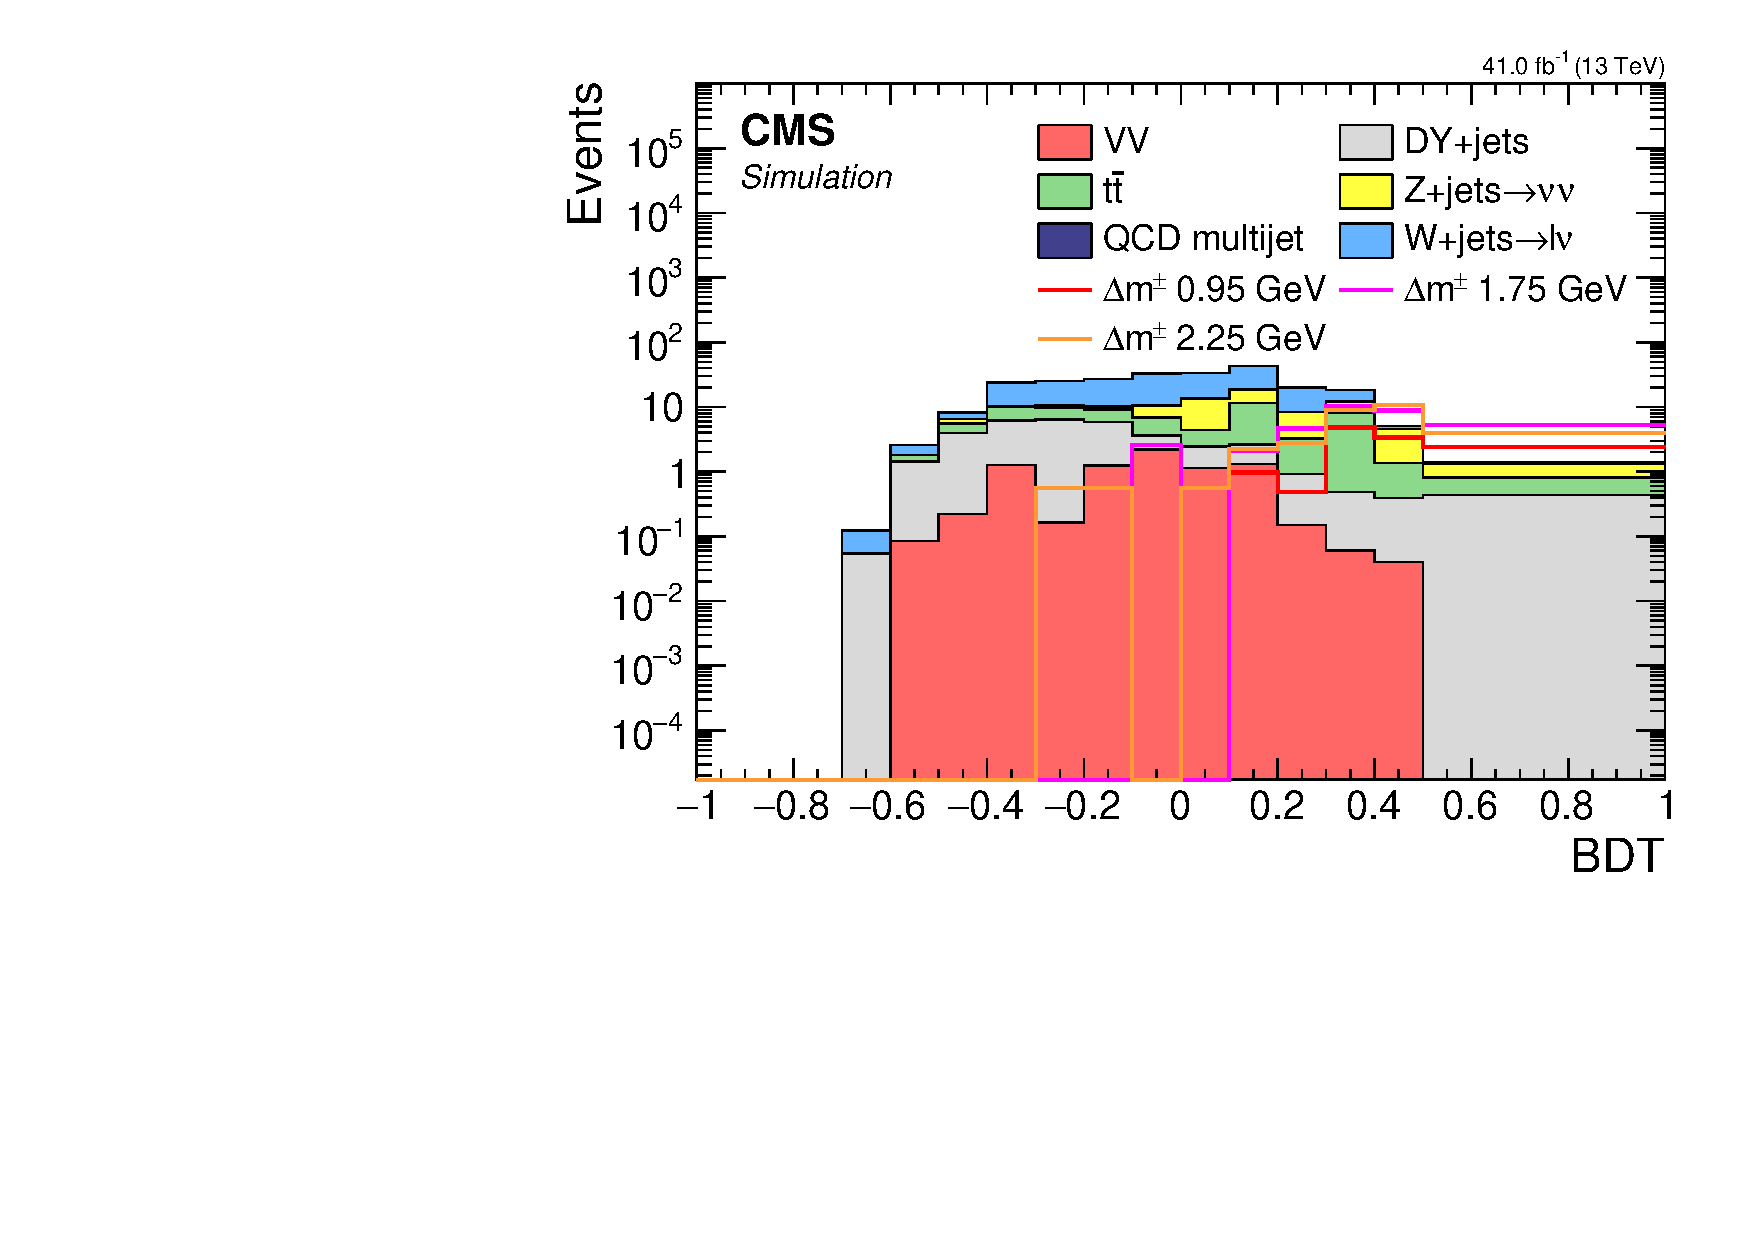
\includegraphics[width=0.48\linewidth]{plots/dilepton_muons_2017/none_custom_dilepBDTCorrJetNoMultIso10Dr0.6_log.pdf} \,
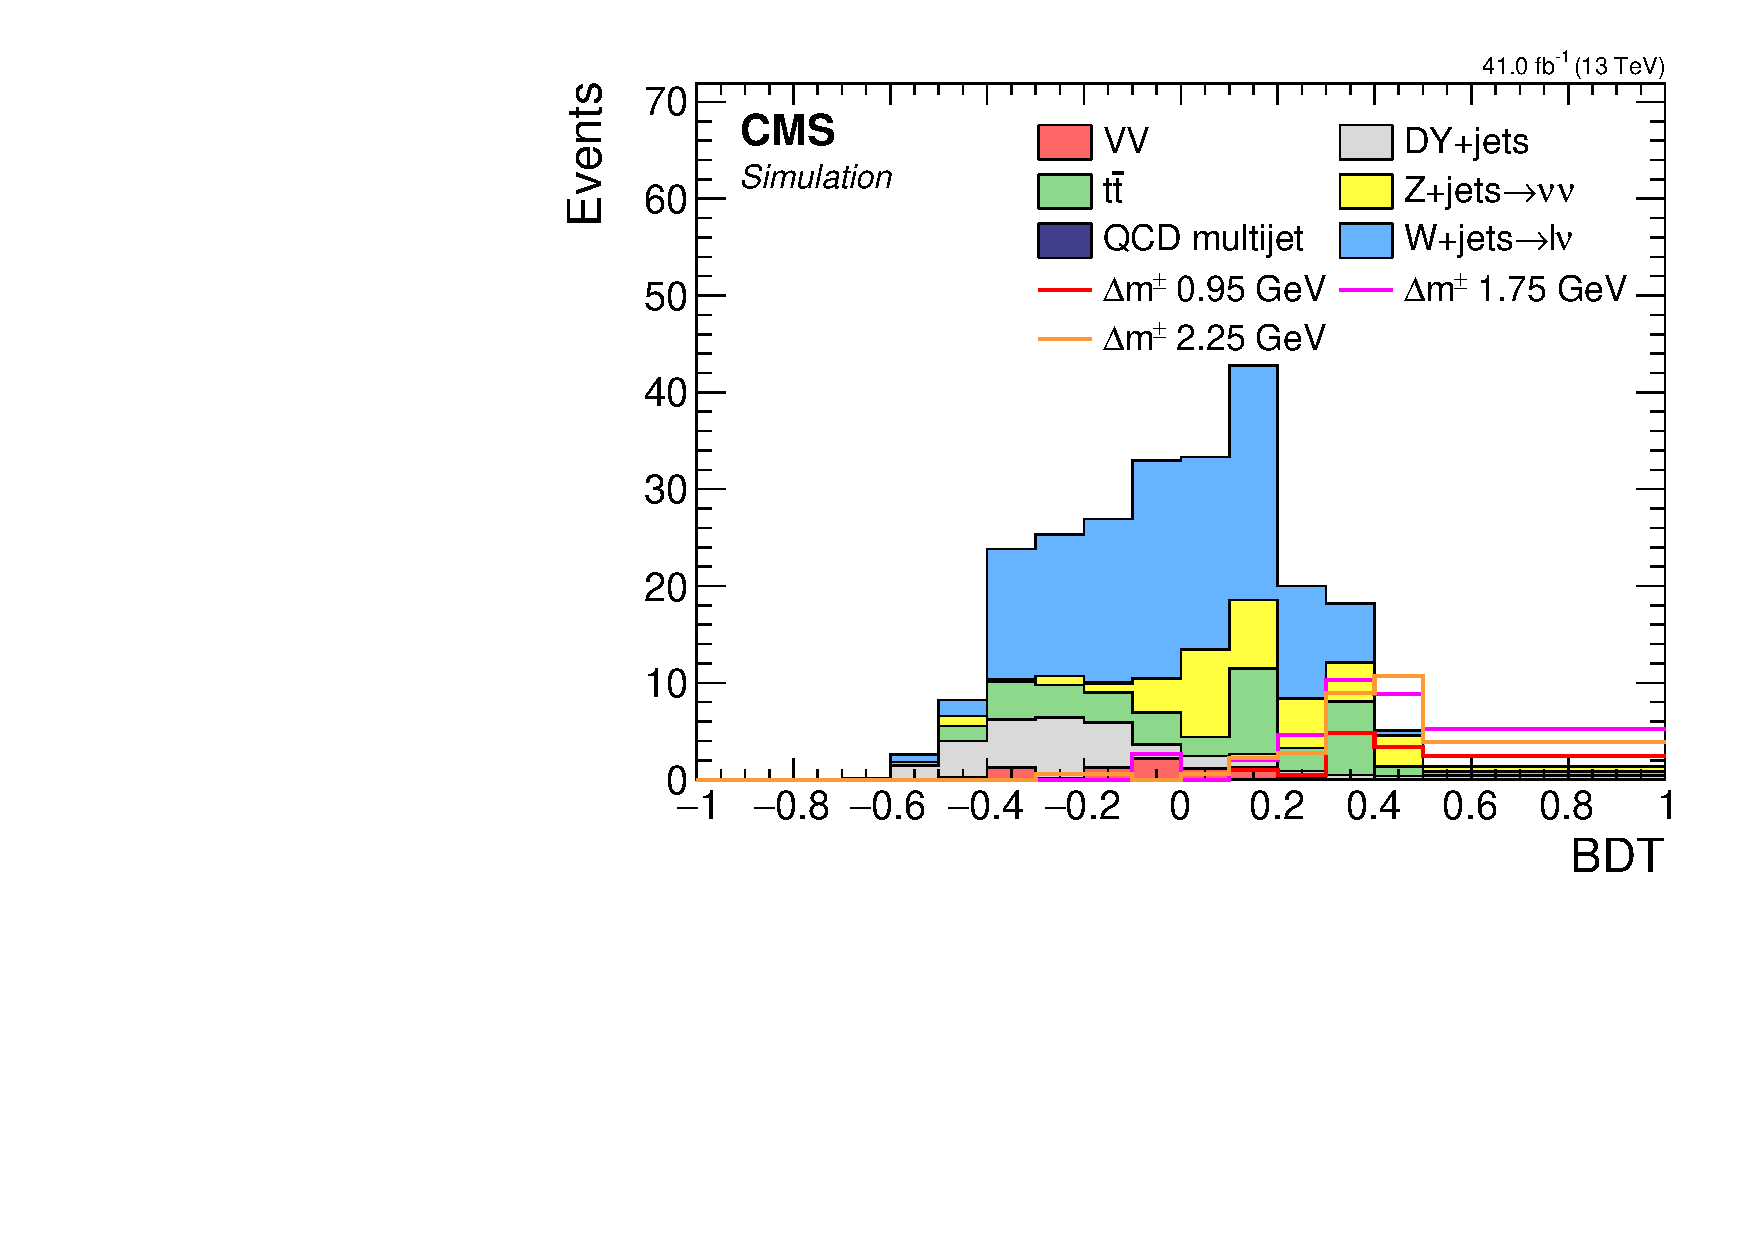
\includegraphics[width=0.48\linewidth]{plots/dilepton_muons_2017/none_custom_dilepBDTCorrJetNoMultIso10Dr0.6.pdf} \\


\caption[Dimuon simulation BDT output]{Dimuon 2017 simulation BDT output in log scale (left) and linear scale (right).}
\label{fig:dimuon-bdt-sim-output}
\end{figure}


\begin{figure}[!htb]
\centering
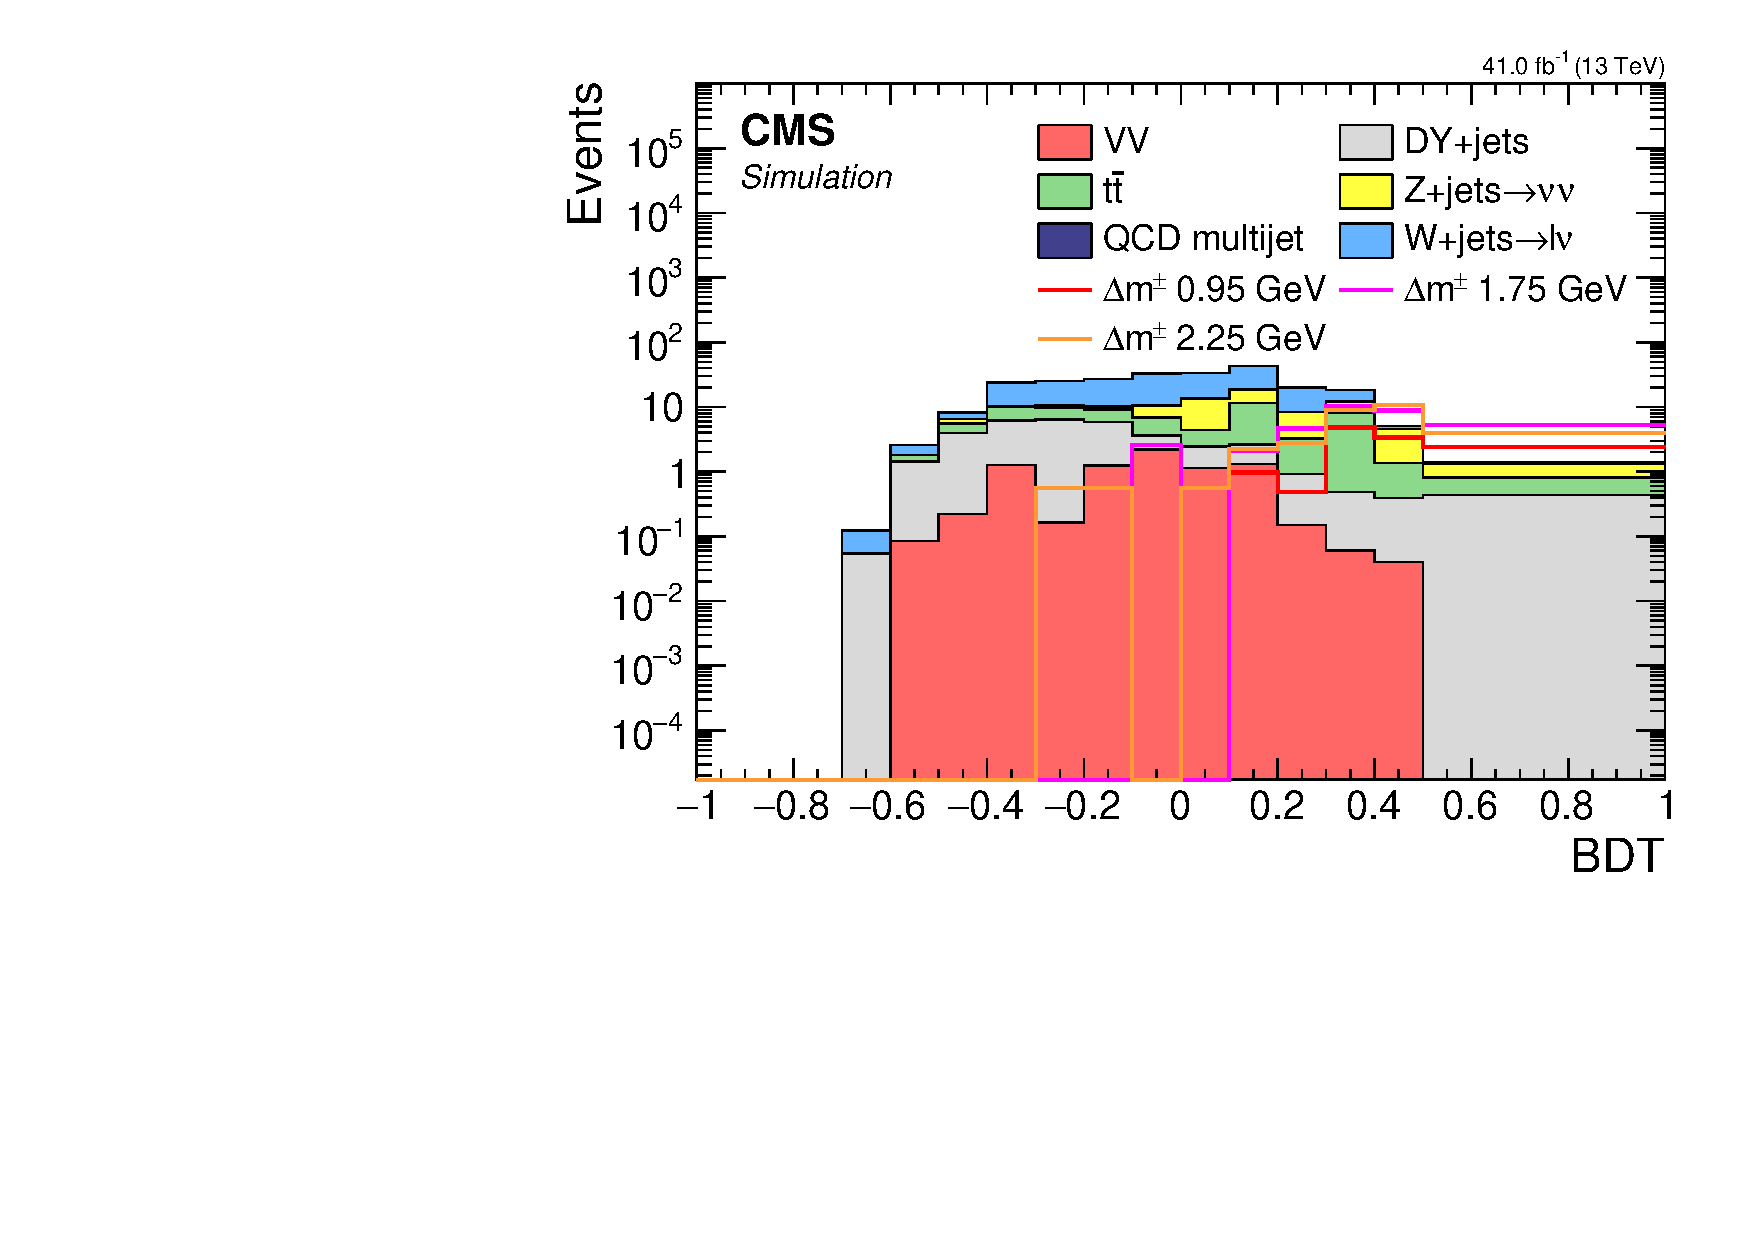
\includegraphics[width=0.48\linewidth]{plots/dilepton_muons_2017/none_custom_dilepBDTCorrJetNoMultIso10Dr0.6_log.pdf} \,
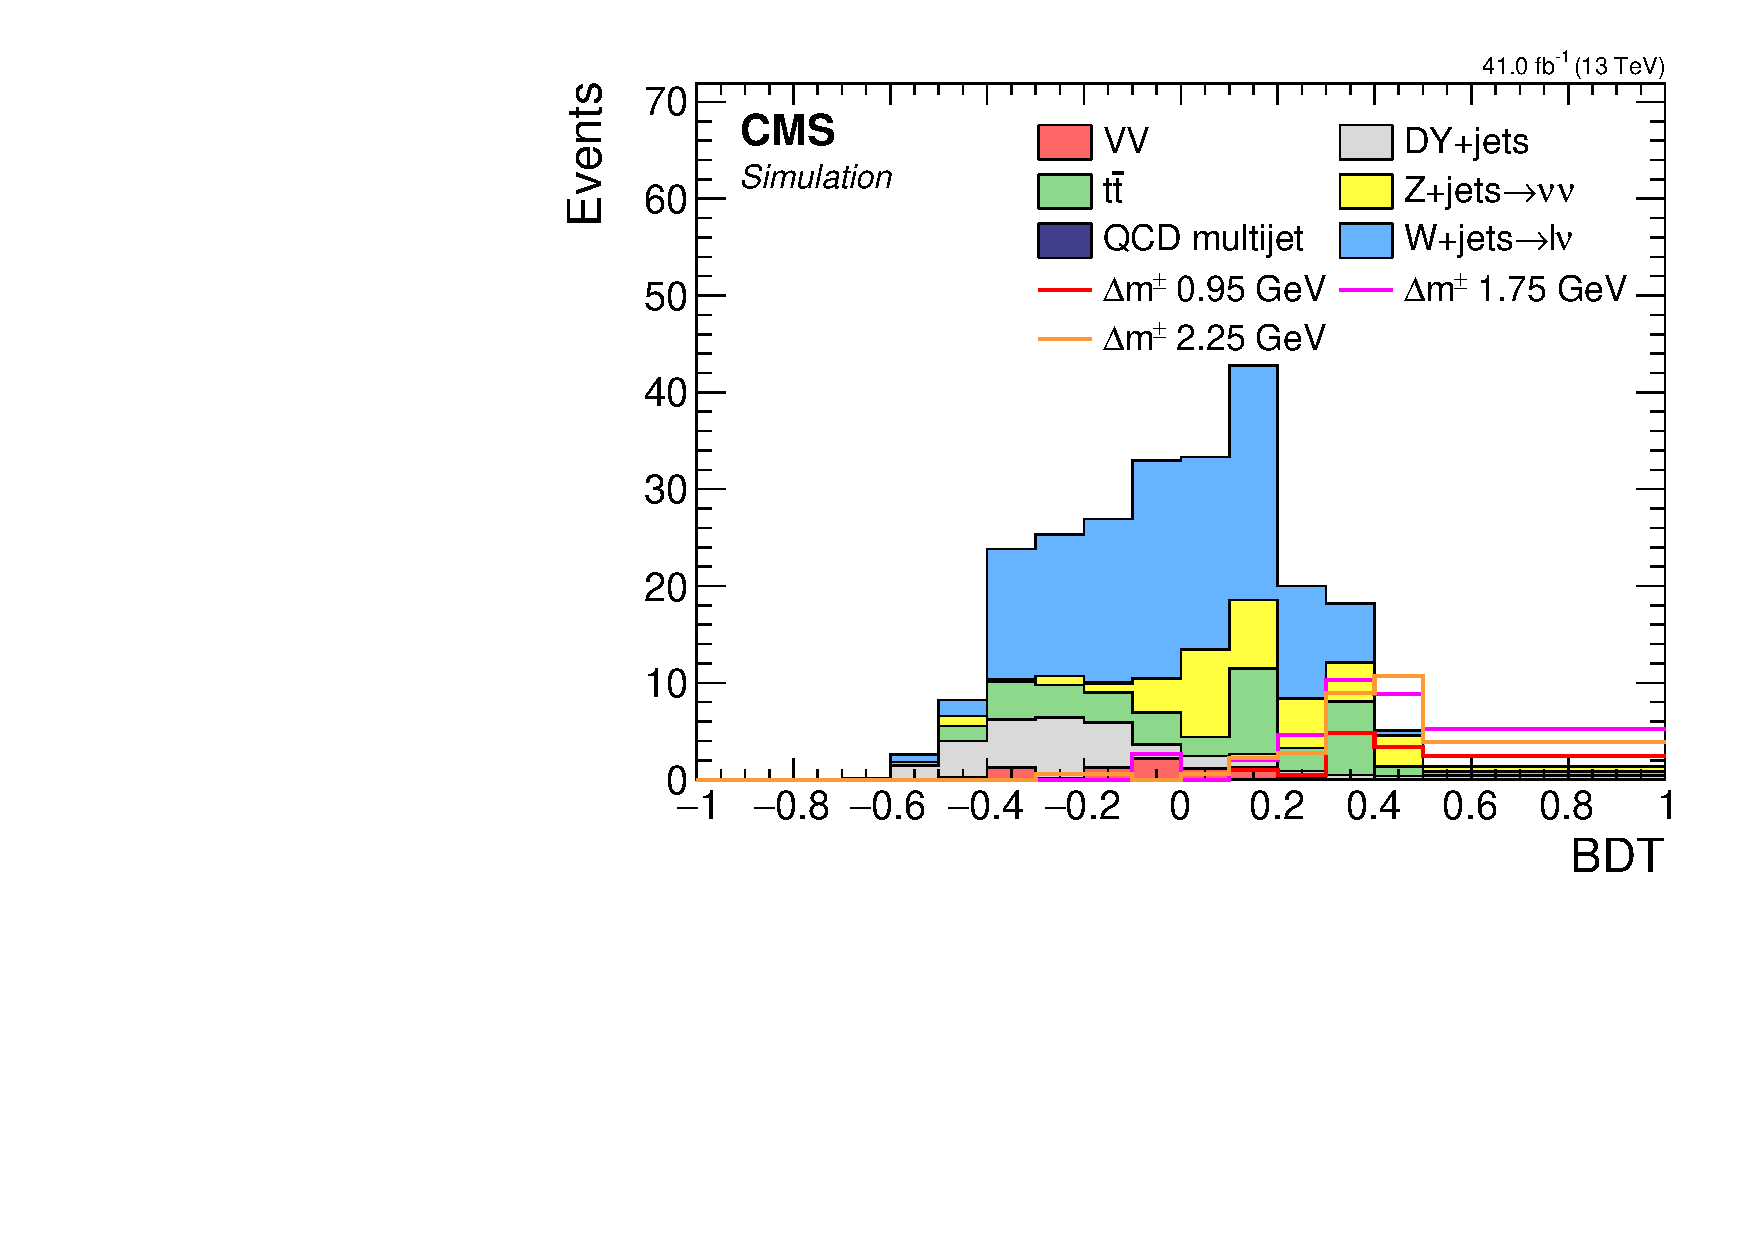
\includegraphics[width=0.48\linewidth]{plots/dilepton_muons_2017/none_custom_dilepBDTCorrJetNoMultIso10Dr0.6.pdf} \\


\caption[Dimuon simulation BDT output jetty tautau]{Dimuon 2017 simulation BDT output in log scale (left) and linear scale (right).  Composition split into...}
\label{fig:dimuon-bdt-sim-output-jetty-tautau}
\end{figure}



\begin{figure}[!htb]
\centering
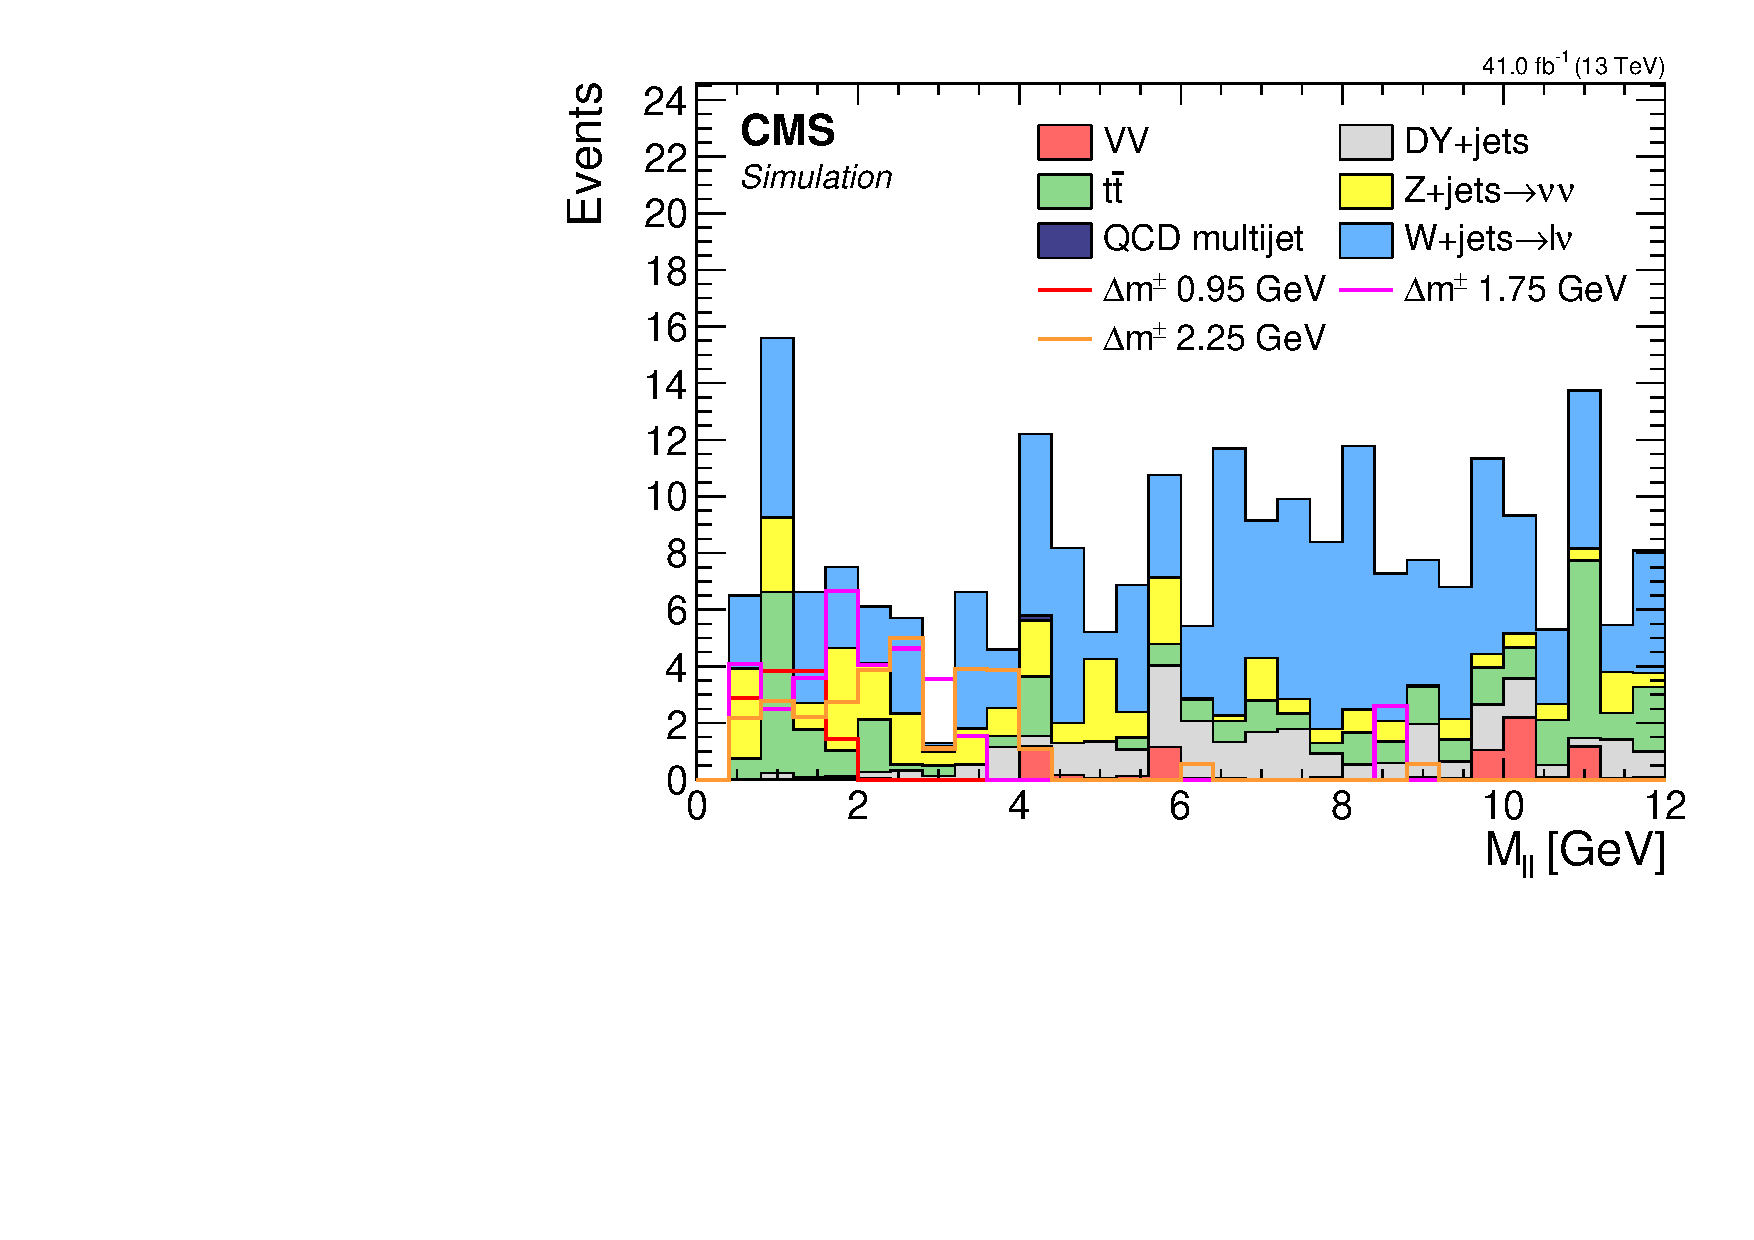
\includegraphics[width=0.48\linewidth]{plots/dilepton_muons_2017/none_invMassCorrJetNoMultIso10Dr0.6.pdf} \,
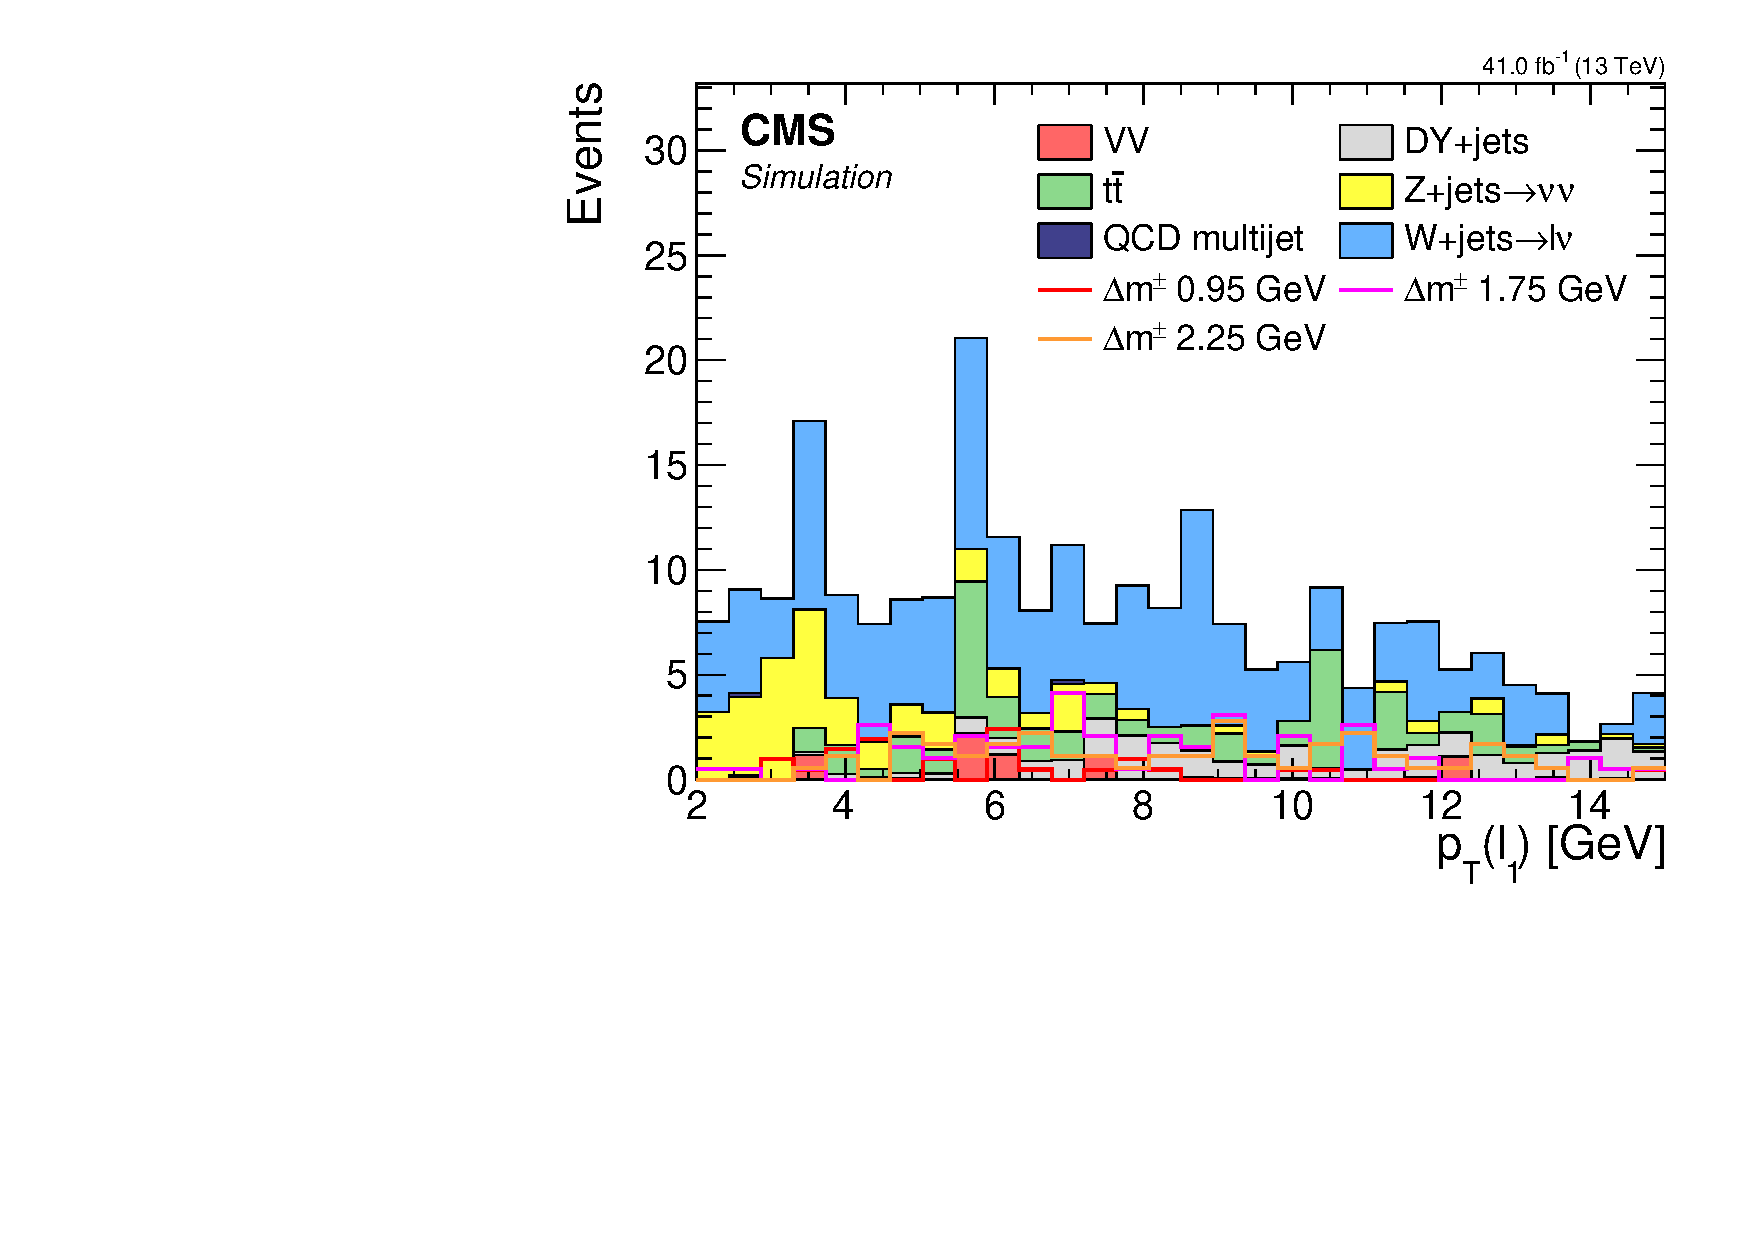
\includegraphics[width=0.48\linewidth]{plots/dilepton_muons_2017/none_leptonsCorrJetNoMultIso10Dr0.6[0].Pt(.pdf} \\

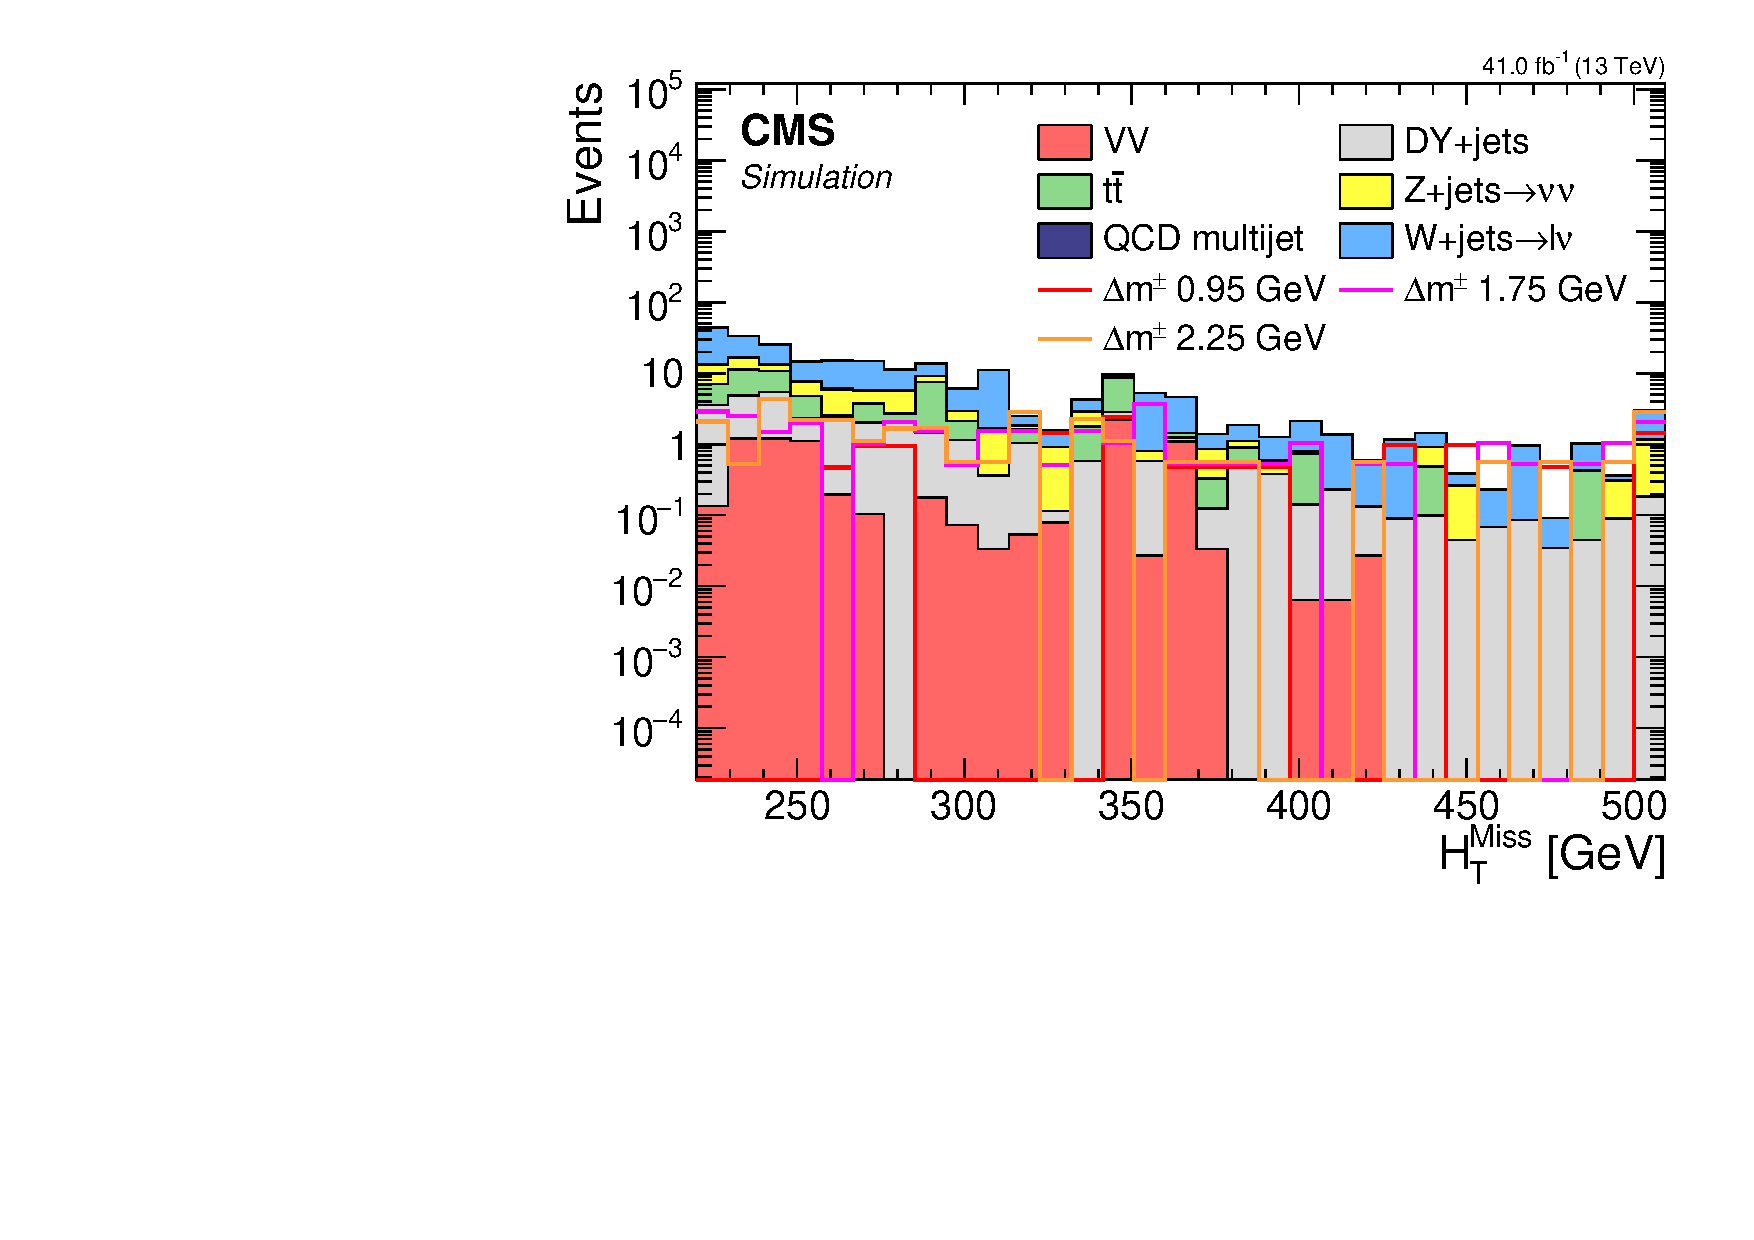
\includegraphics[width=0.48\linewidth]{plots/dilepton_muons_2017/none_MHT_log.pdf} \,
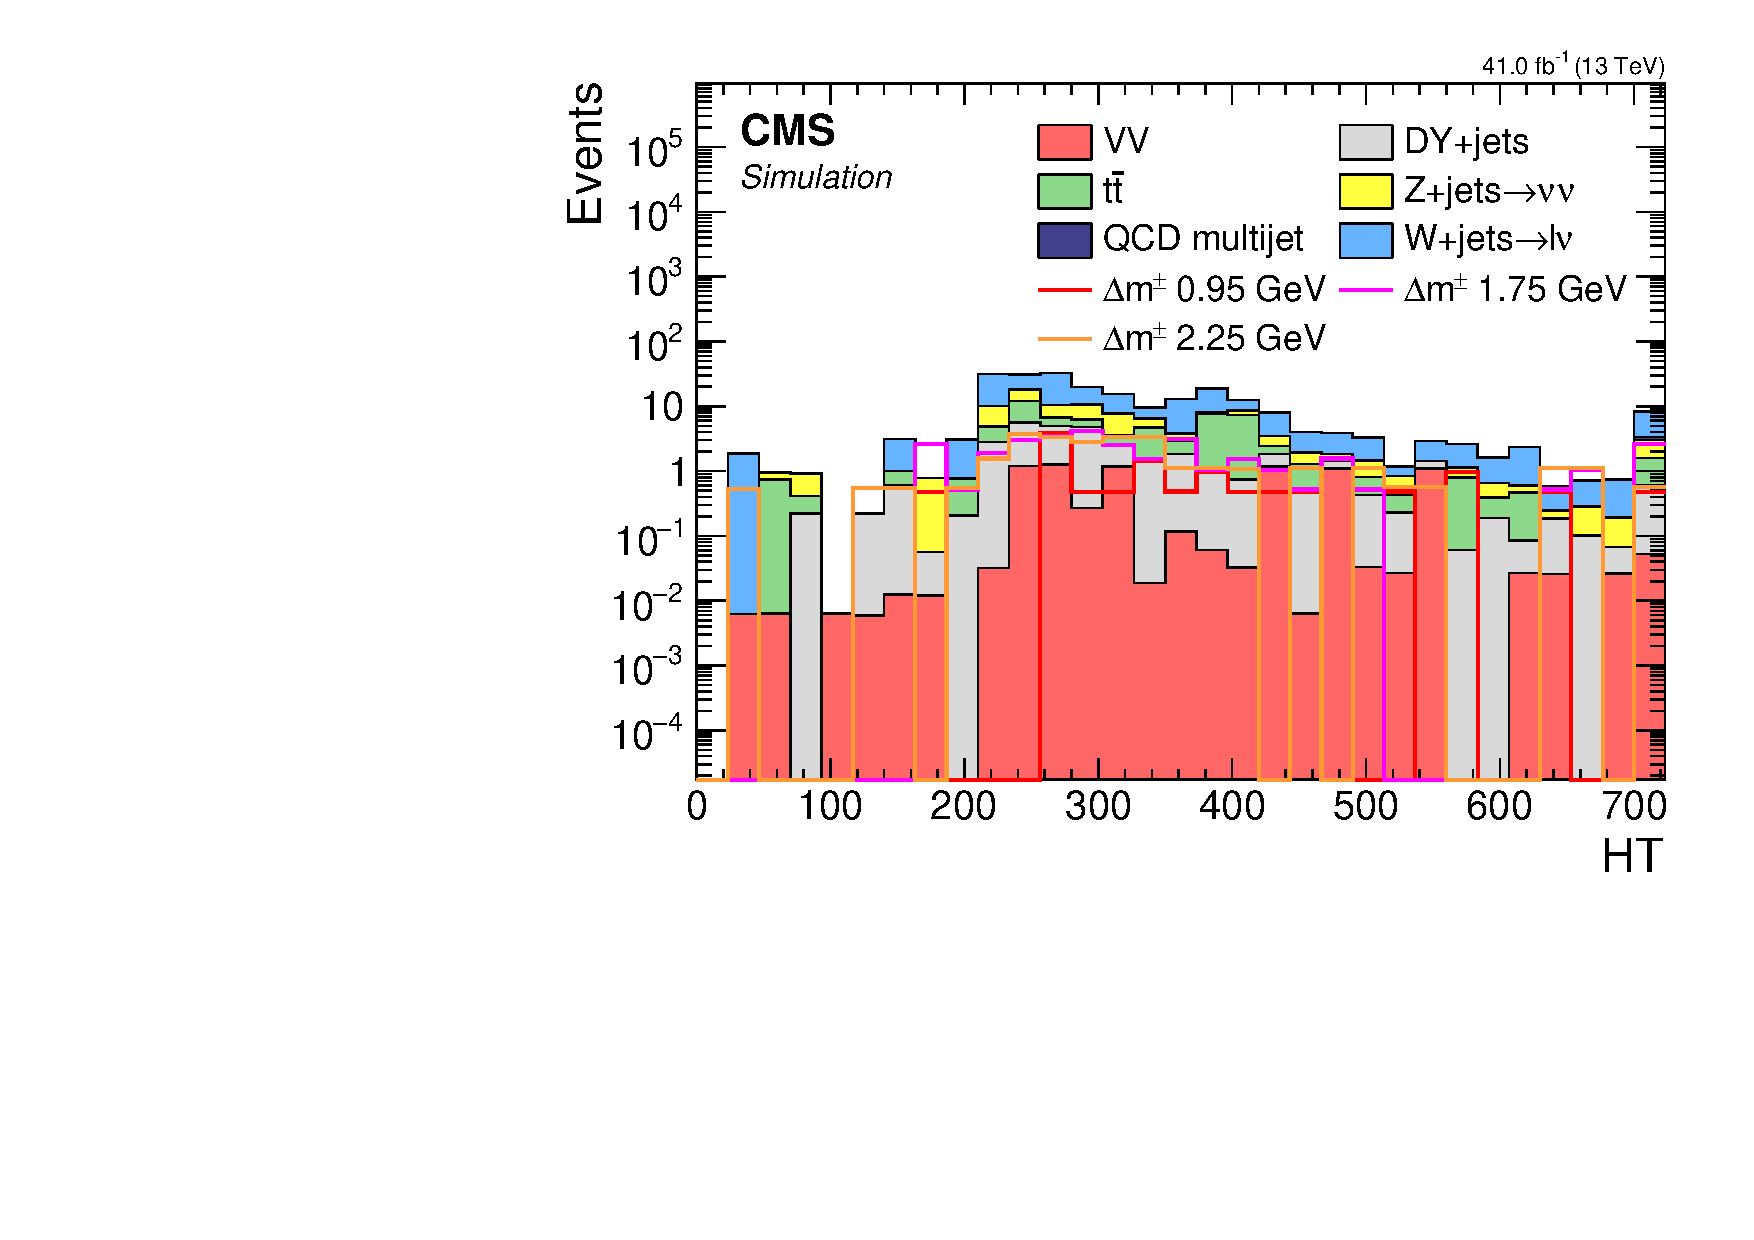
\includegraphics[width=0.48\linewidth]{plots/dilepton_muons_2017/none_HT_log.pdf} \\


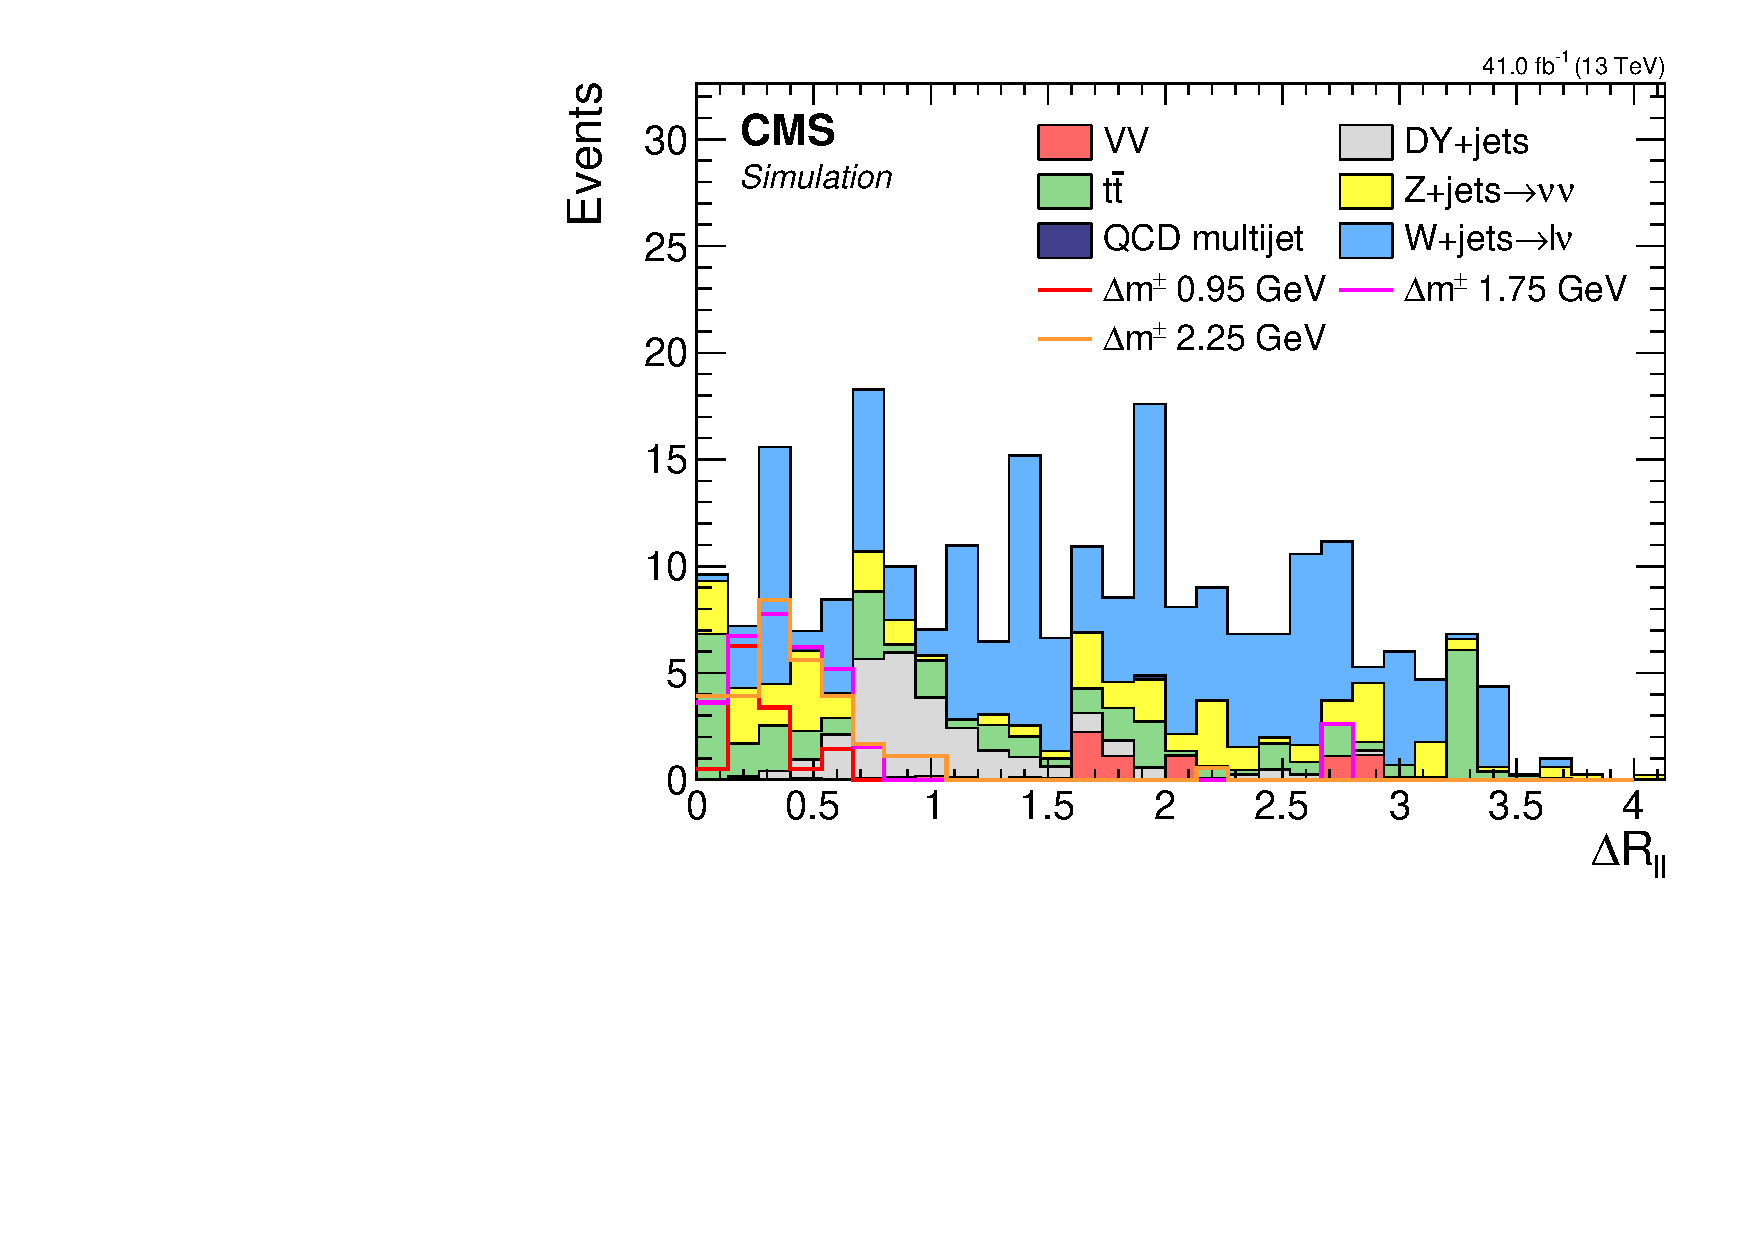
\includegraphics[width=0.48\linewidth]{plots/dilepton_muons_2017/none_deltaRCorrJetNoMultIso10Dr0.6.pdf} \,
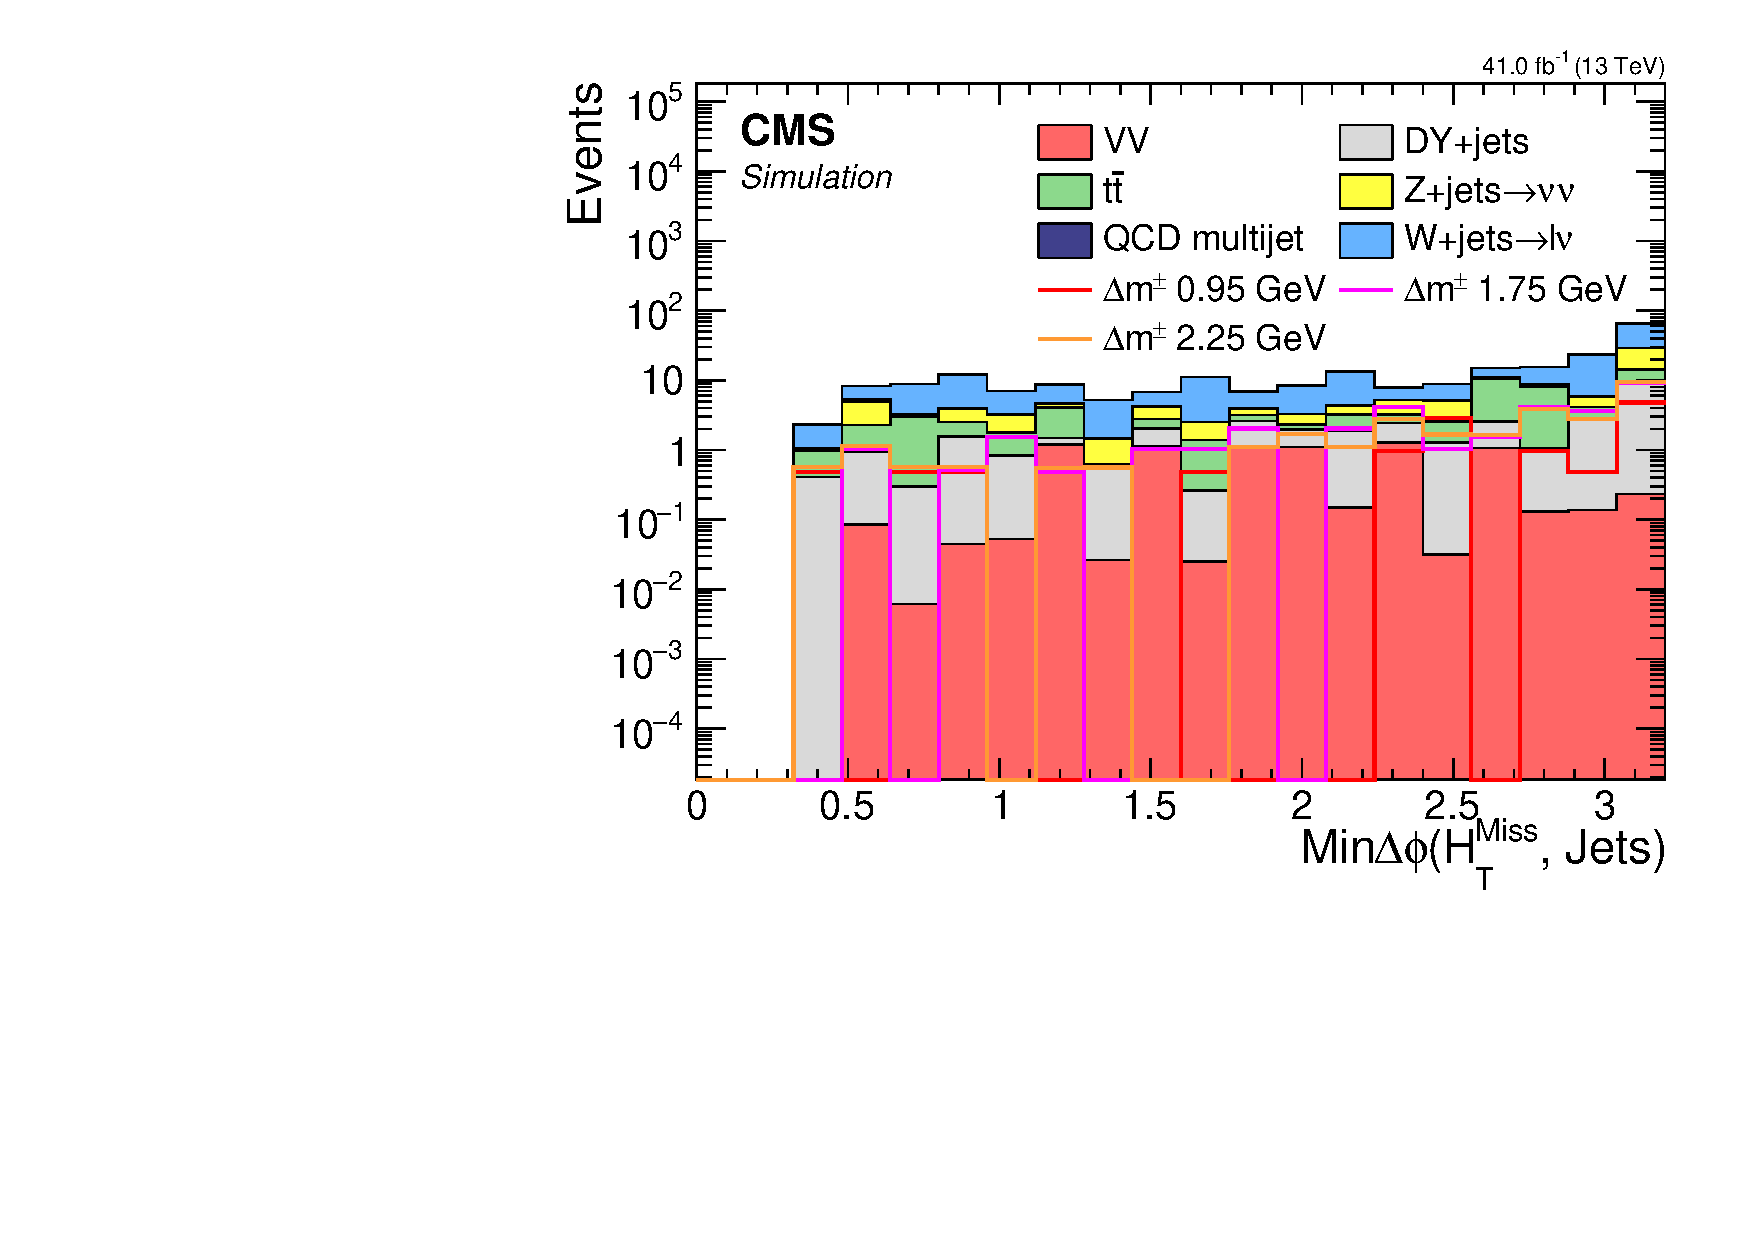
\includegraphics[width=0.48\linewidth]{plots/dilepton_muons_2017/none_MinDeltaPhiMhtJets_log.pdf} \\

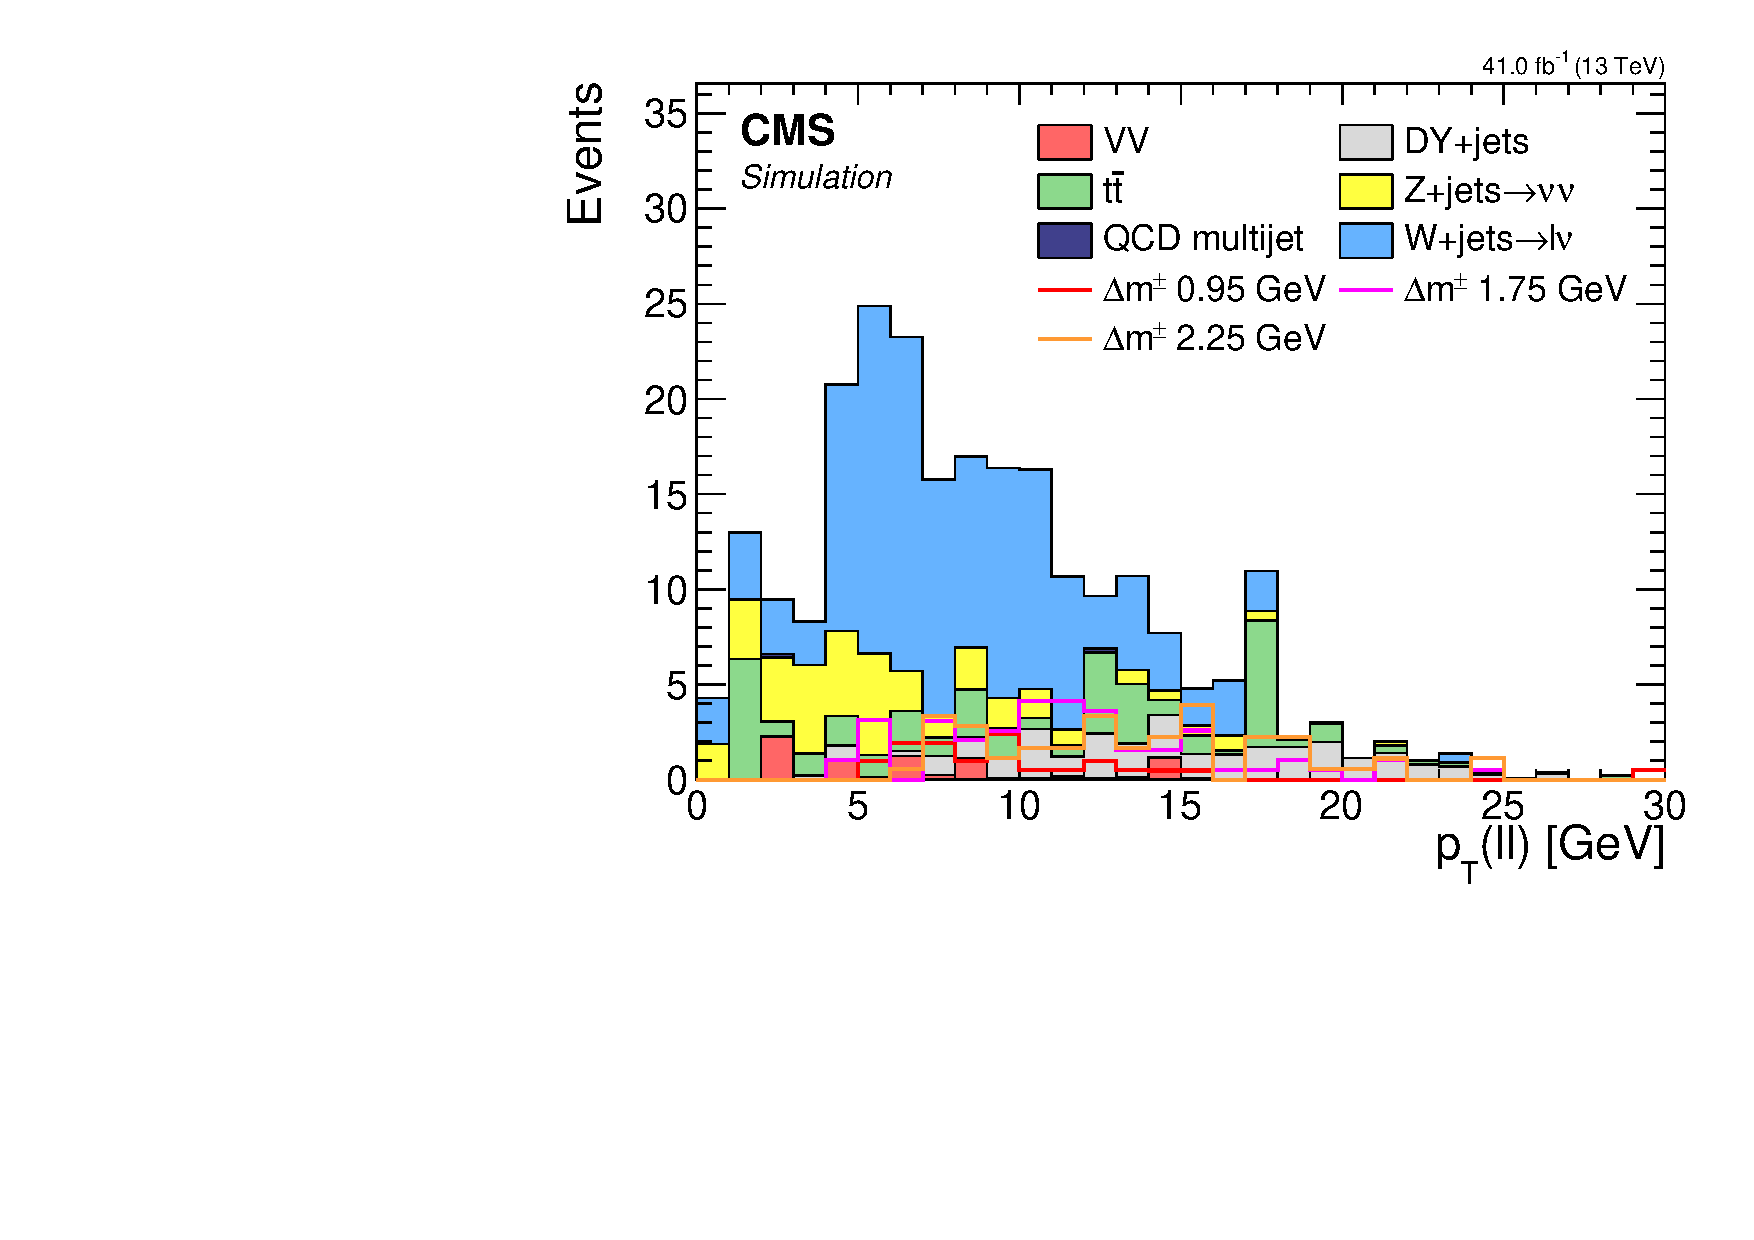
\includegraphics[width=0.48\linewidth]{plots/dilepton_muons_2017/none_dileptonPtCorrJetNoMultIso10Dr0.6.pdf} \,
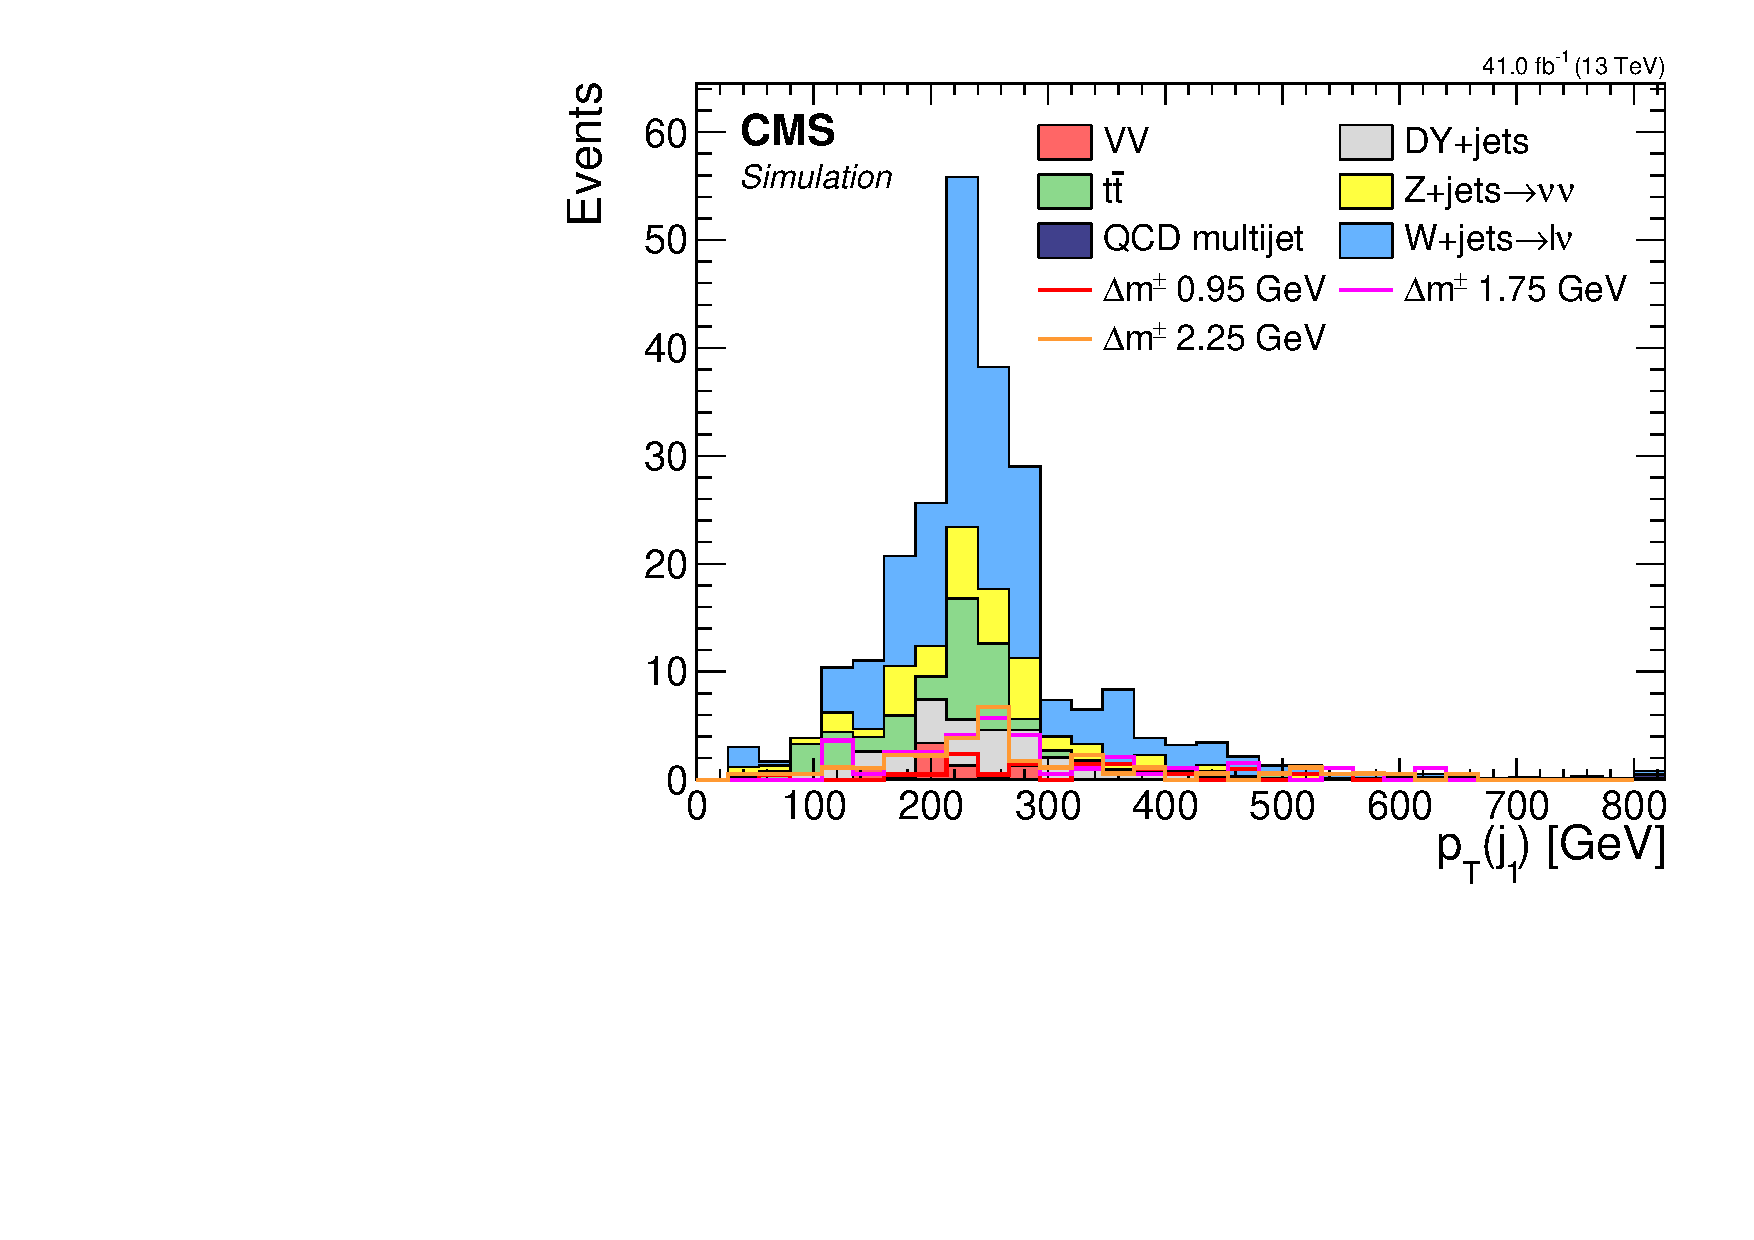
\includegraphics[width=0.48\linewidth]{plots/dilepton_muons_2017/none_LeadingJetPt.pdf} \\



\caption[Dimuon simulation BDT inputs]{Dimuon 2017 simulation BDT inputs for the top 10 ranked observables.}
\label{fig:dimuon-bdt-sim-inputs}
\end{figure}

\fxnote{Add jetty/tautau simulation plot}

\clearpage
\subsubsection{Exclusive track category}

As described before, there are four \glspl{bdt} in the exclusive track category, for each of the two lepton flavors there are two track phases. 

\begin{figure}[!htb]
\centering
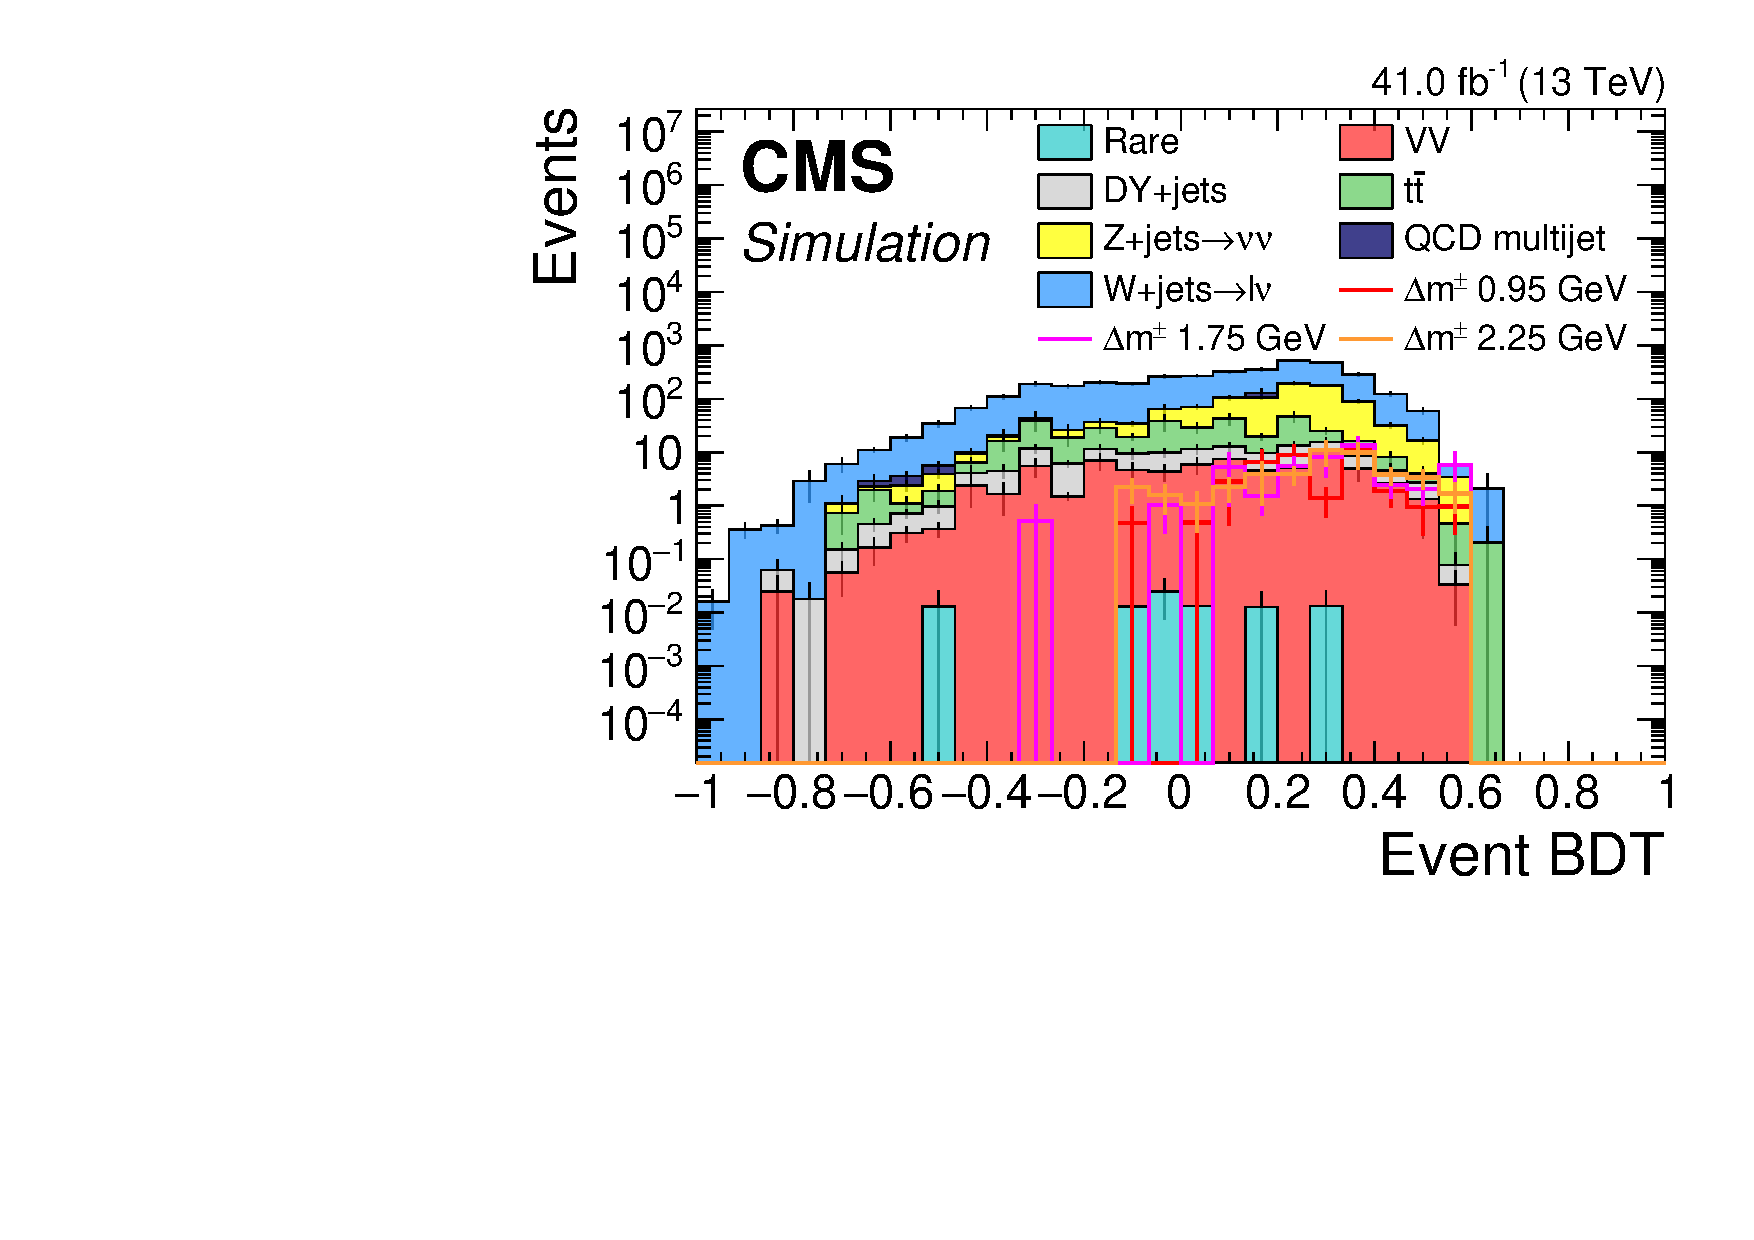
\includegraphics[width=0.48\linewidth]{plots/track_muon_bg_signal/none_exTrack_dilepBDTCorrJetNoMultIso10Dr0.6_log.pdf} \,
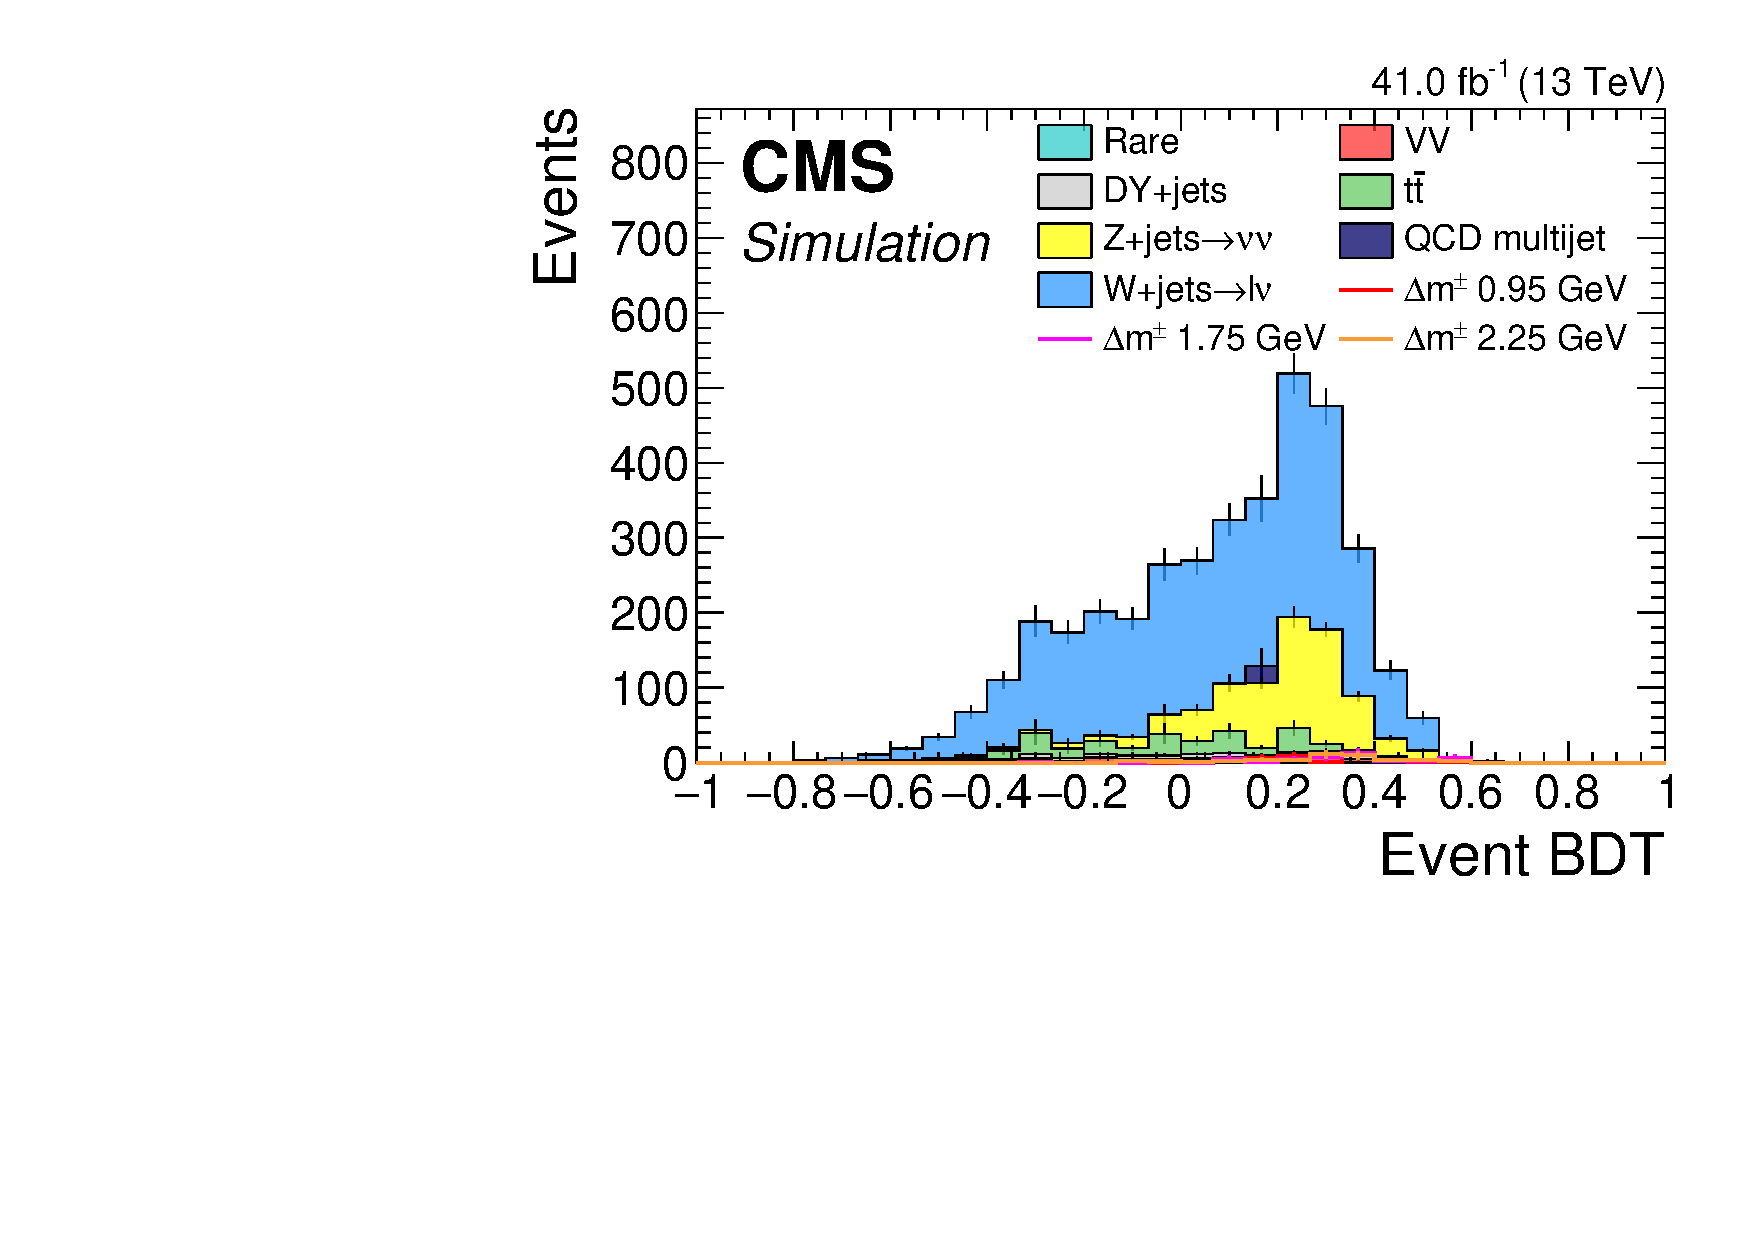
\includegraphics[width=0.48\linewidth]{plots/track_muon_bg_signal/none_exTrack_dilepBDTCorrJetNoMultIso10Dr0.6.pdf} \\

\caption[Exclusive track plus muon 2017 simulation BDT output]{Exclusive track plus muon category 2017 simulation BDT output in log scale (left) and linear scale (right).}
\label{fig:exclusive-track-bdt-sim-output}
\end{figure}

The muon flavor in phase 1 is chosen to represent background composition in the exclusive track category in order to avoid repetition, and can be seen in Figure~\ref{fig:exclusive-track-bdt-sim-output}. Figure~\ref{fig:exclusive-track-muon-bdt-sim-inputs} shows the top eight input observables to the \gls{bdt}, ranked by importance for the training. It is weighted to 2017 luminosity and uses 2017 simulation. A few signal points are also plotted in order to point to the signal-like regions of phase space.

\begin{figure}[!htb]
\centering
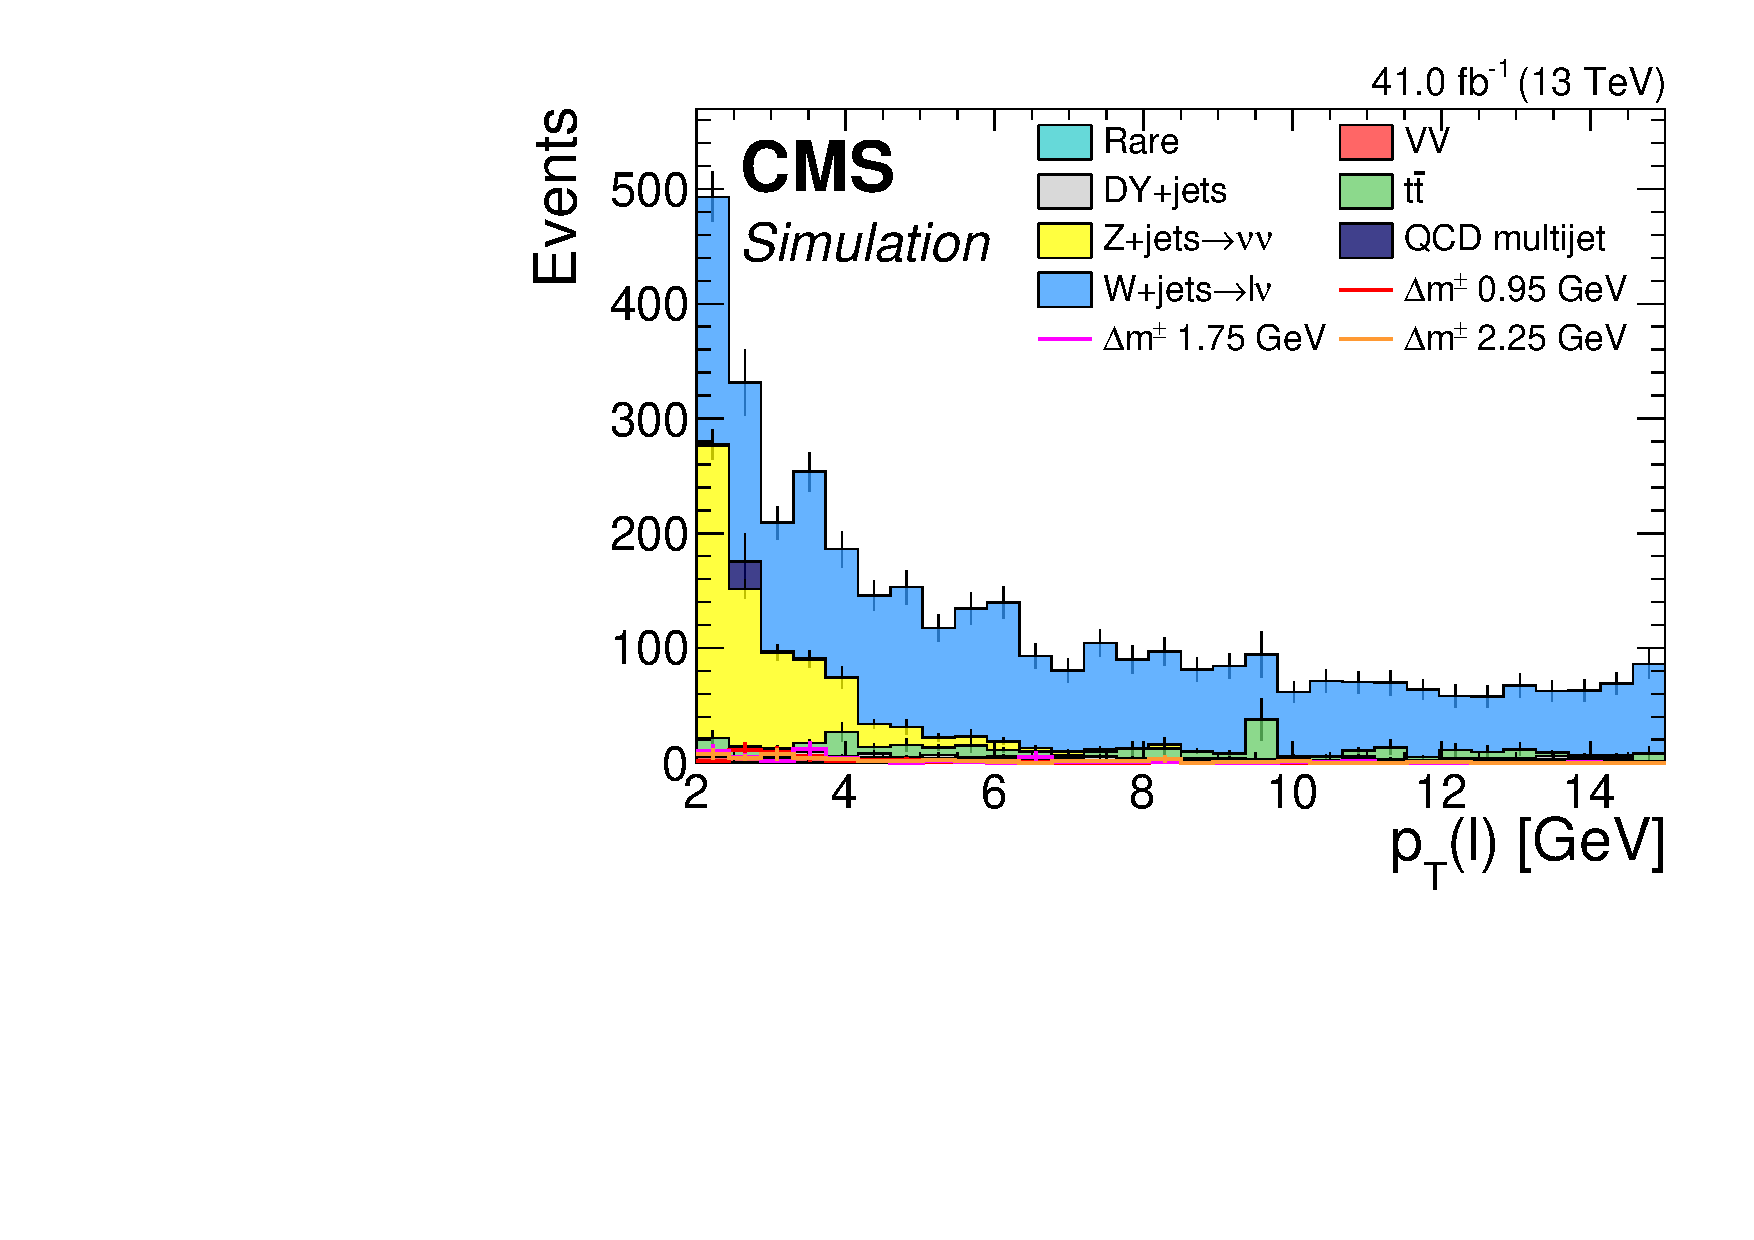
\includegraphics[width=0.48\linewidth]{plots/track_muon_bg_signal/none_leptonCorrJetNoMultIso10Dr0.6.Pt().pdf} \,
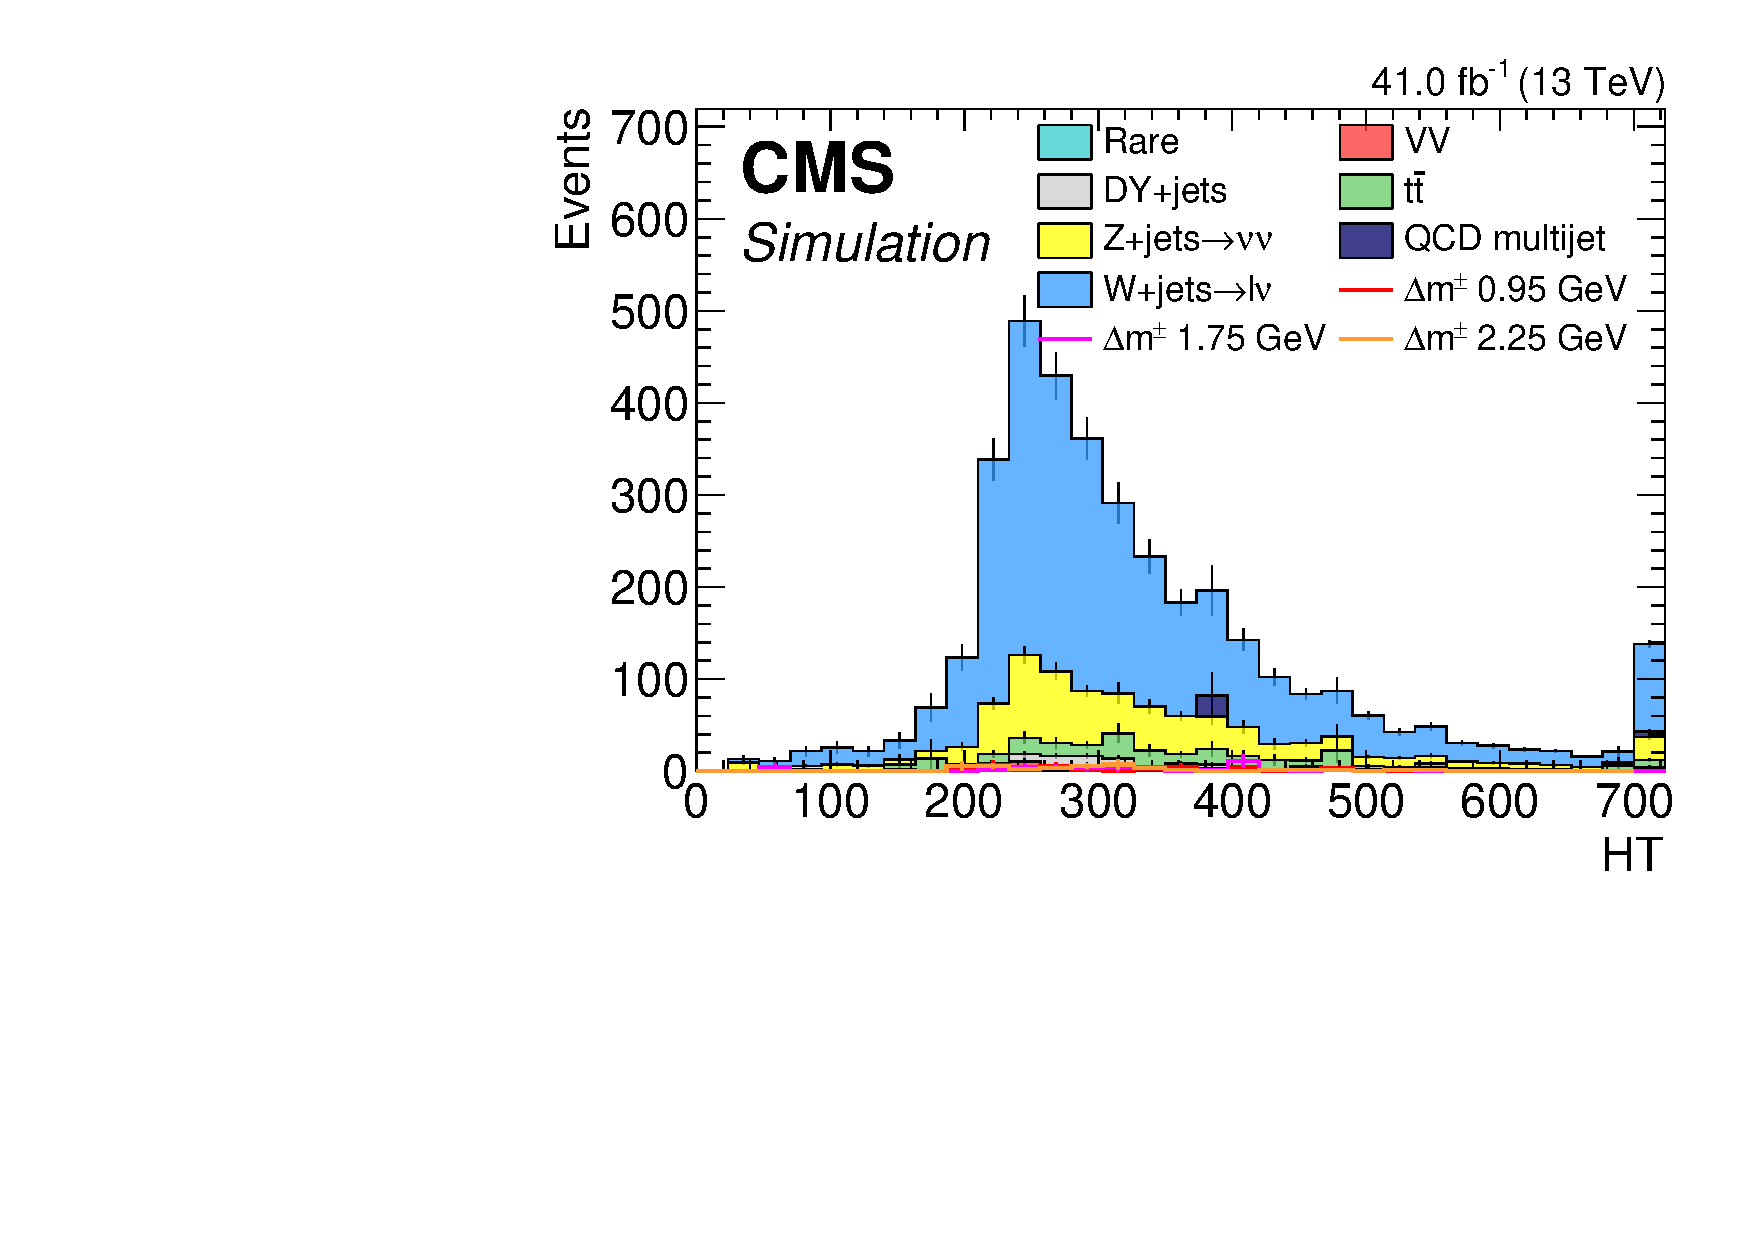
\includegraphics[width=0.48\linewidth]{plots/track_muon_bg_signal/none_HT.pdf} \\
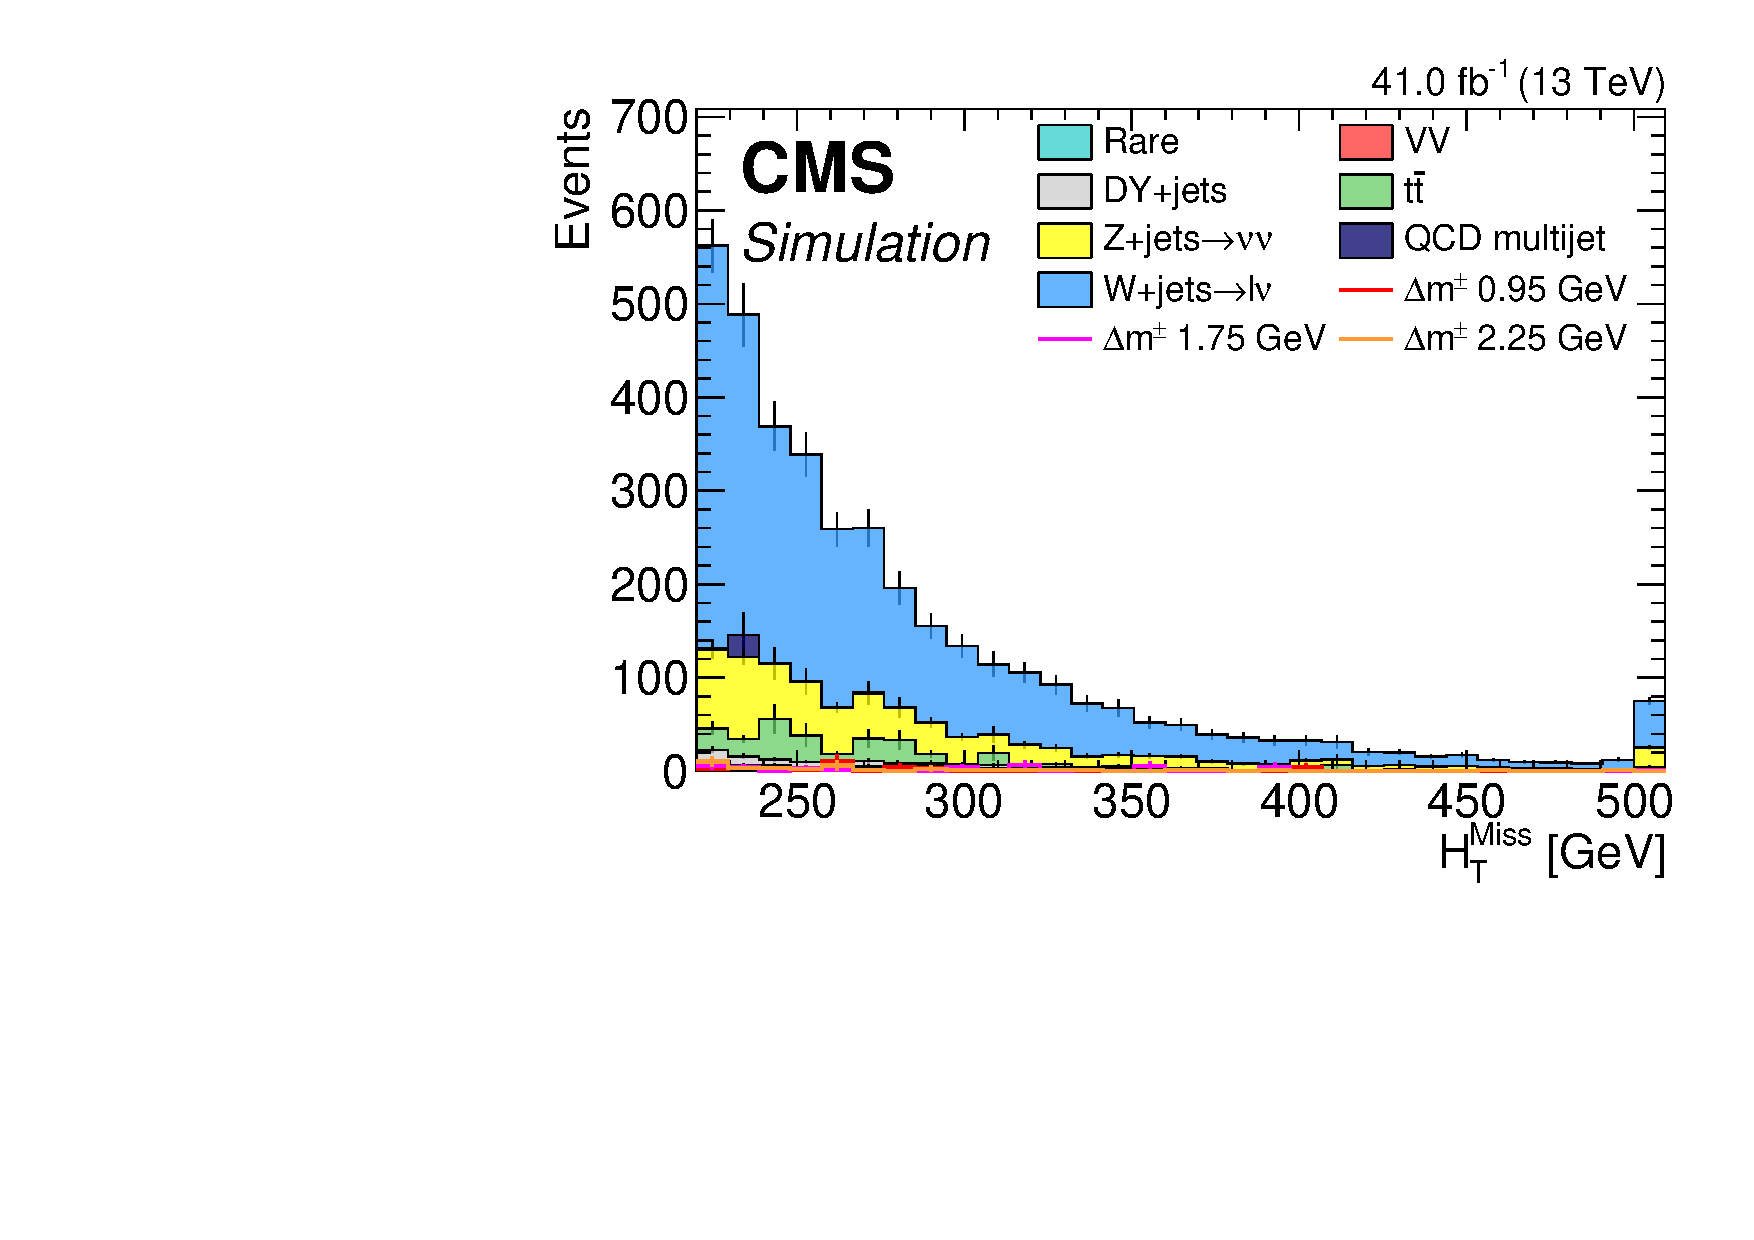
\includegraphics[width=0.48\linewidth]{plots/track_muon_bg_signal/none_MHT.pdf} \,
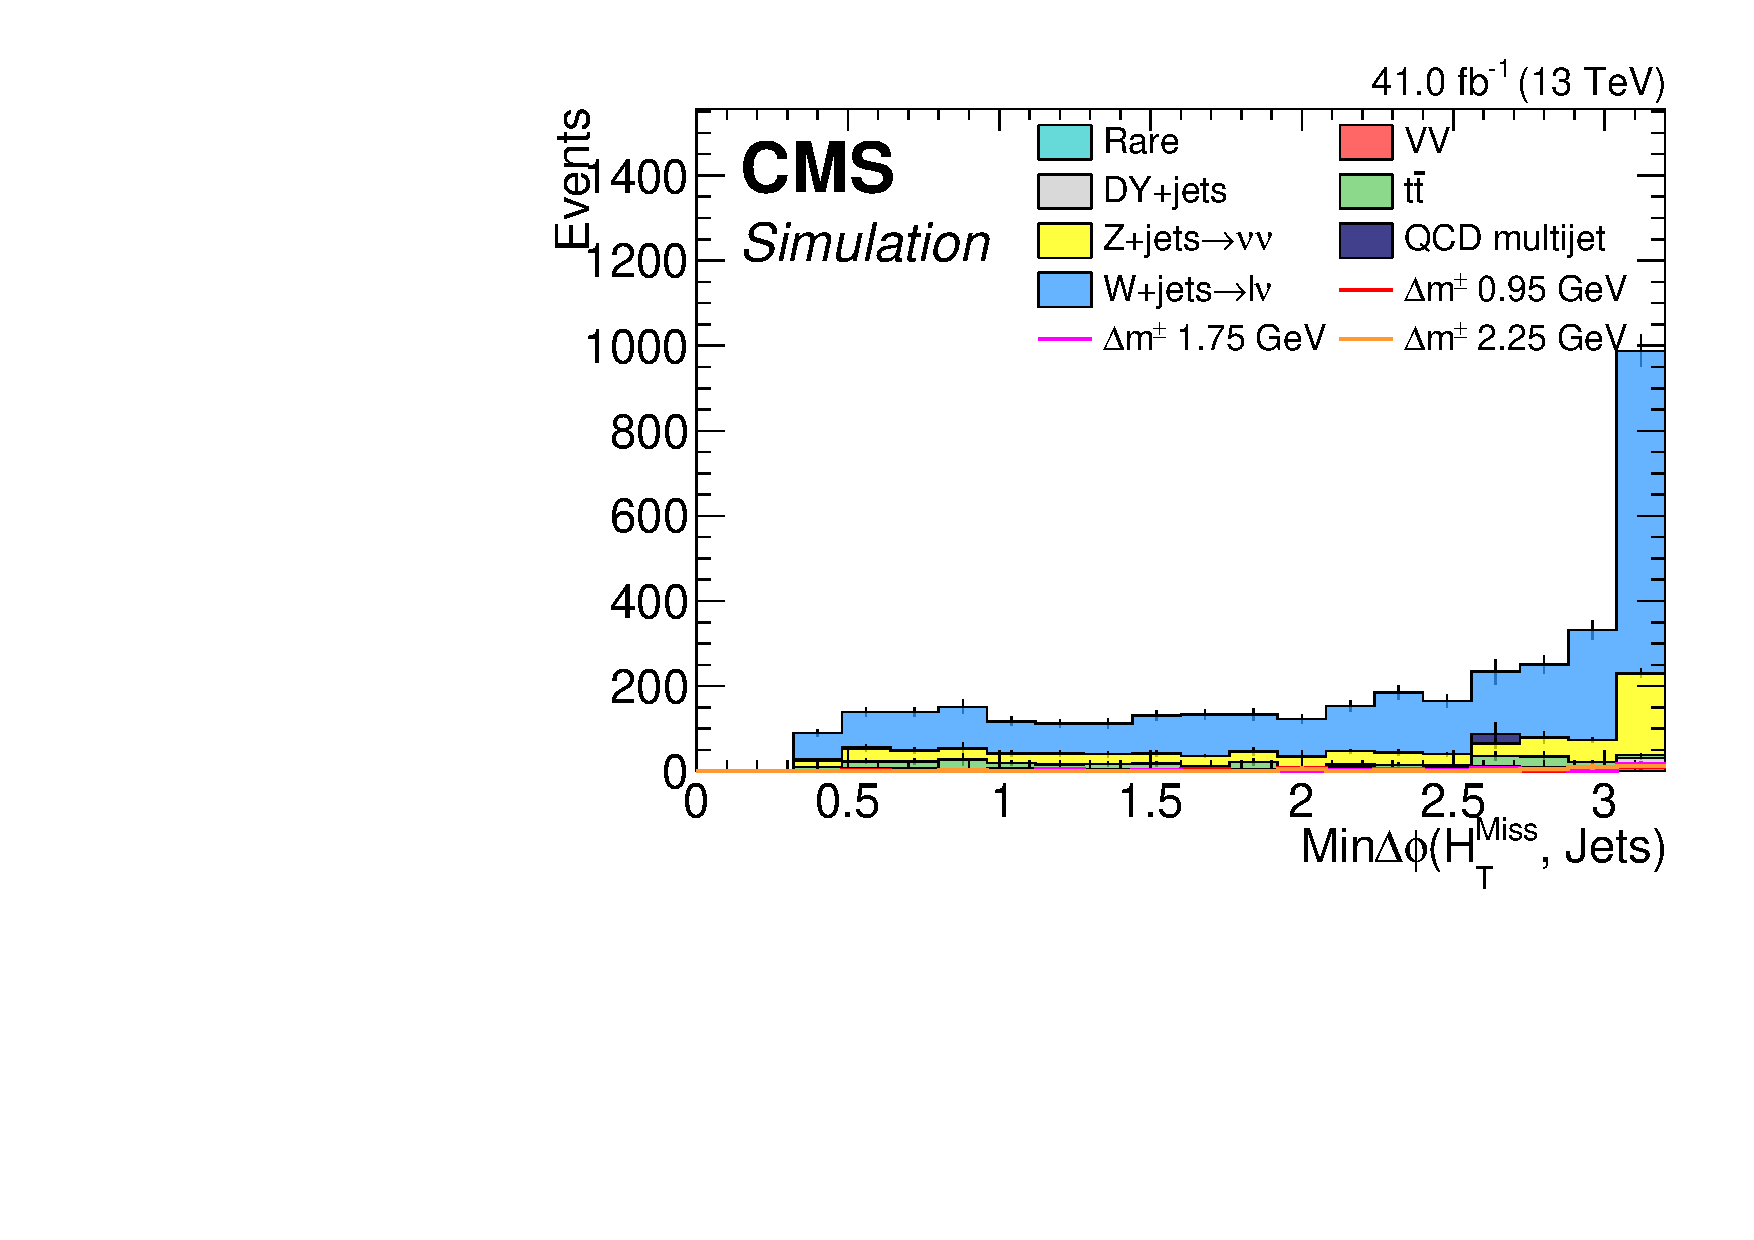
\includegraphics[width=0.48\linewidth]{plots/track_muon_bg_signal/none_MinDeltaPhiMhtJets.pdf} \\
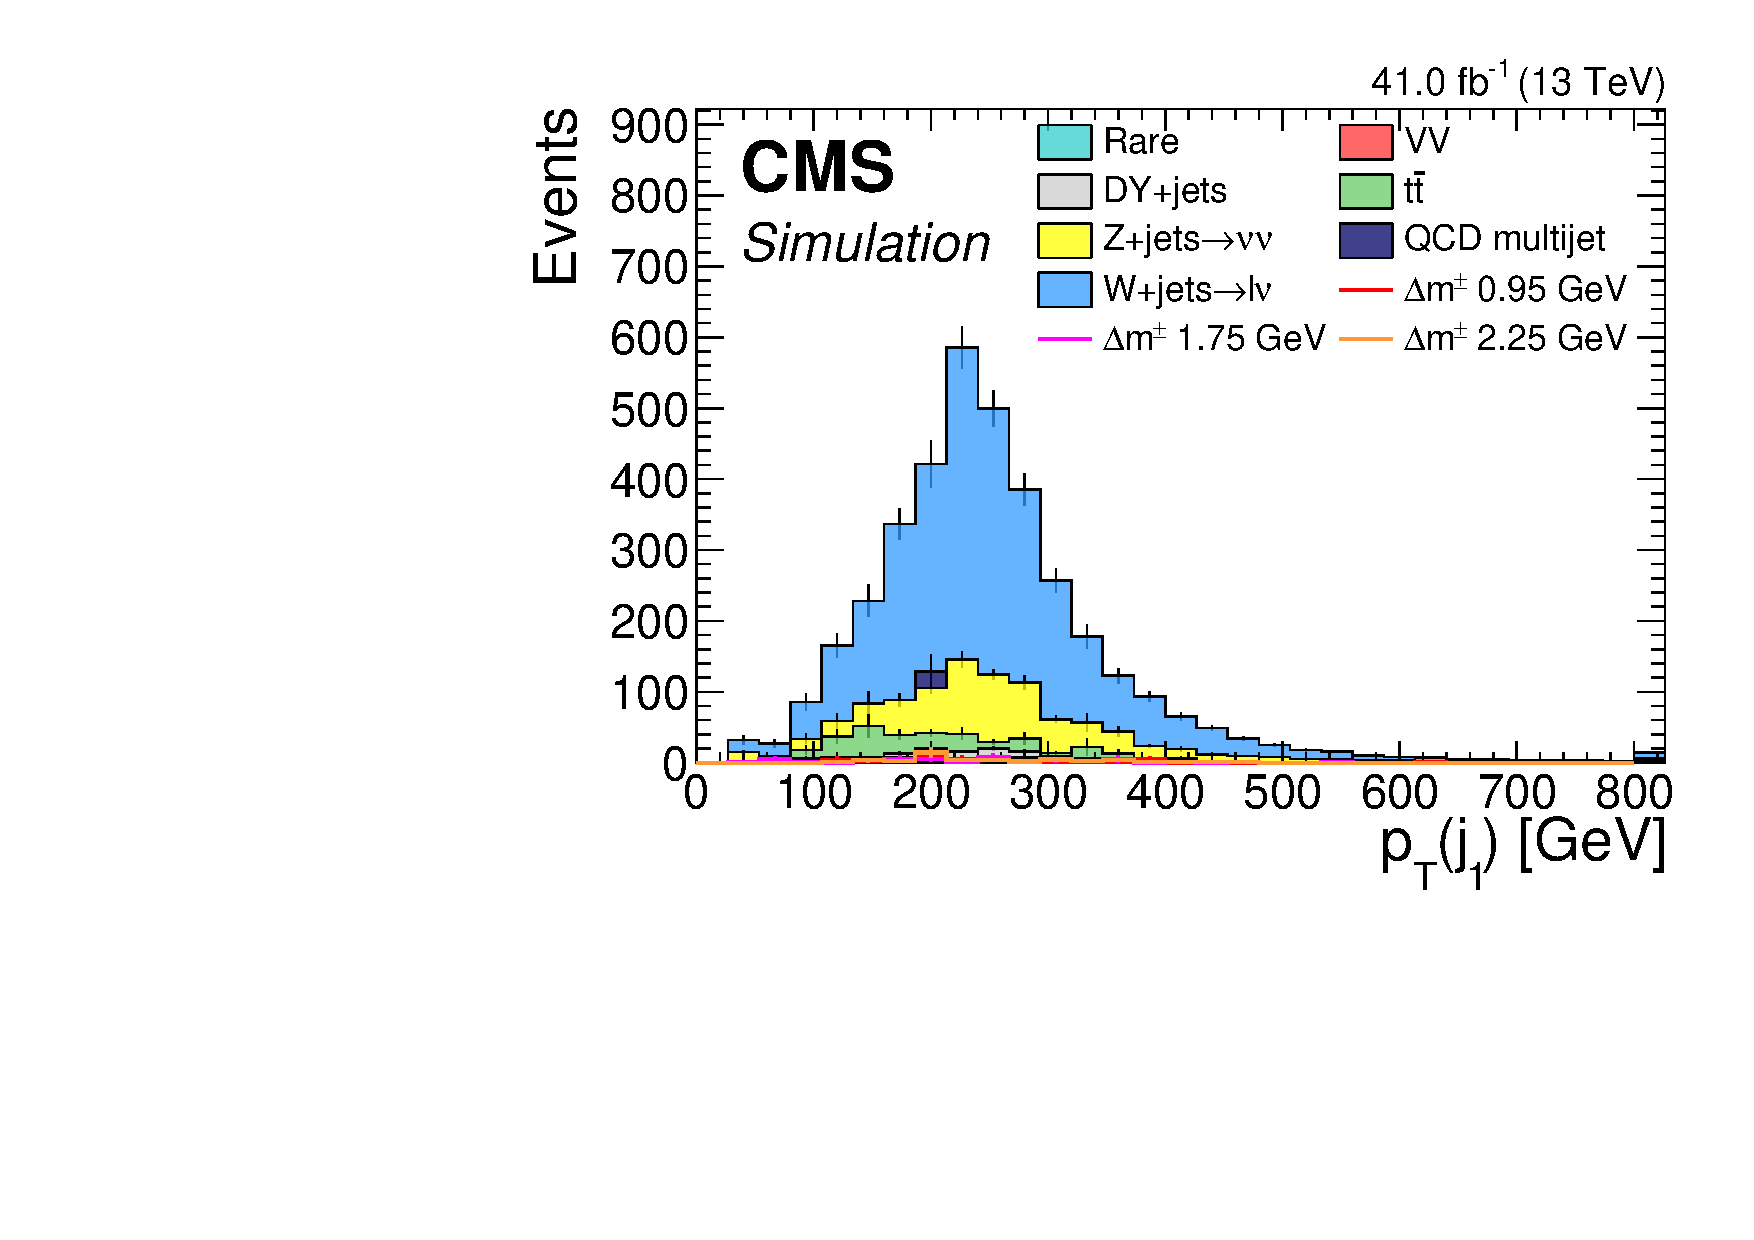
\includegraphics[width=0.48\linewidth]{plots/track_muon_bg_signal/none_LeadingJetPt.pdf} \,
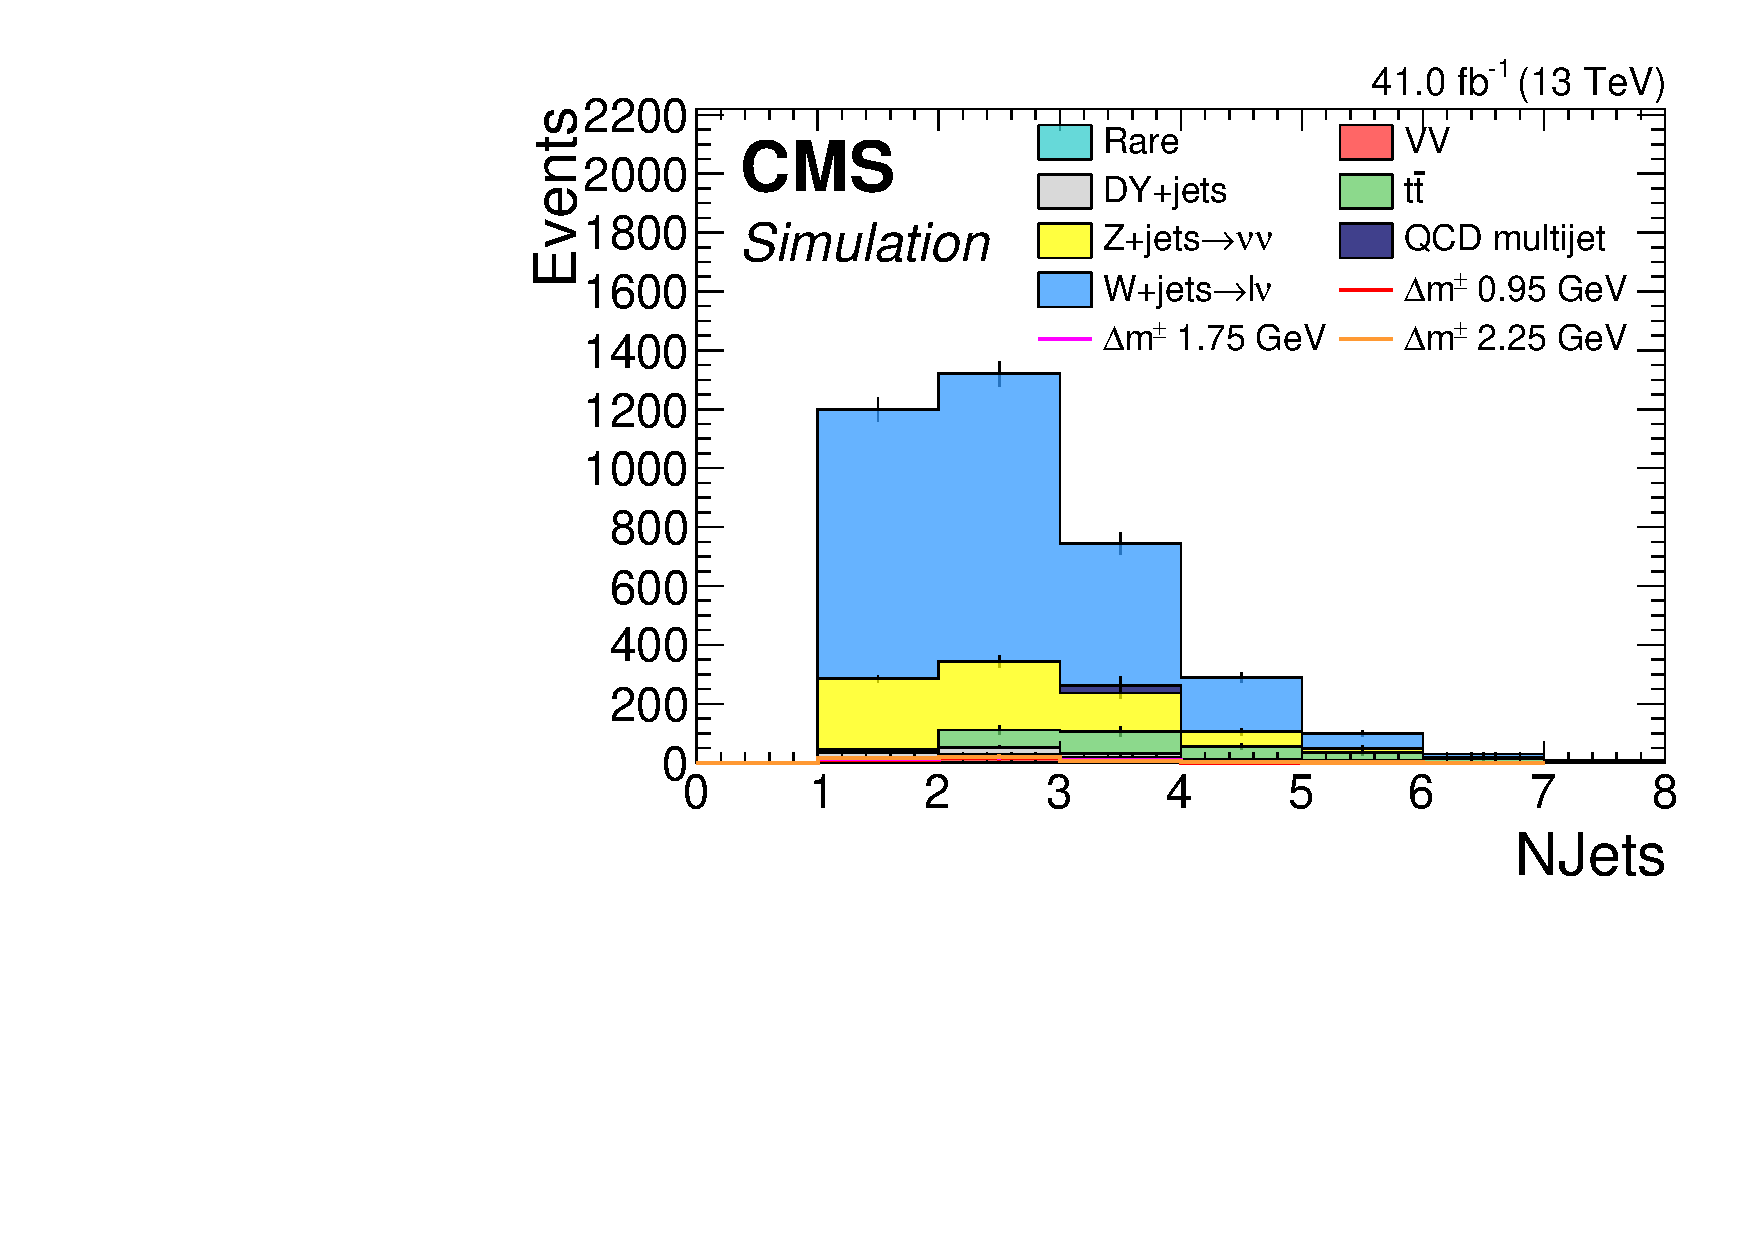
\includegraphics[width=0.48\linewidth]{plots/track_muon_bg_signal/none_NJets.pdf} \\
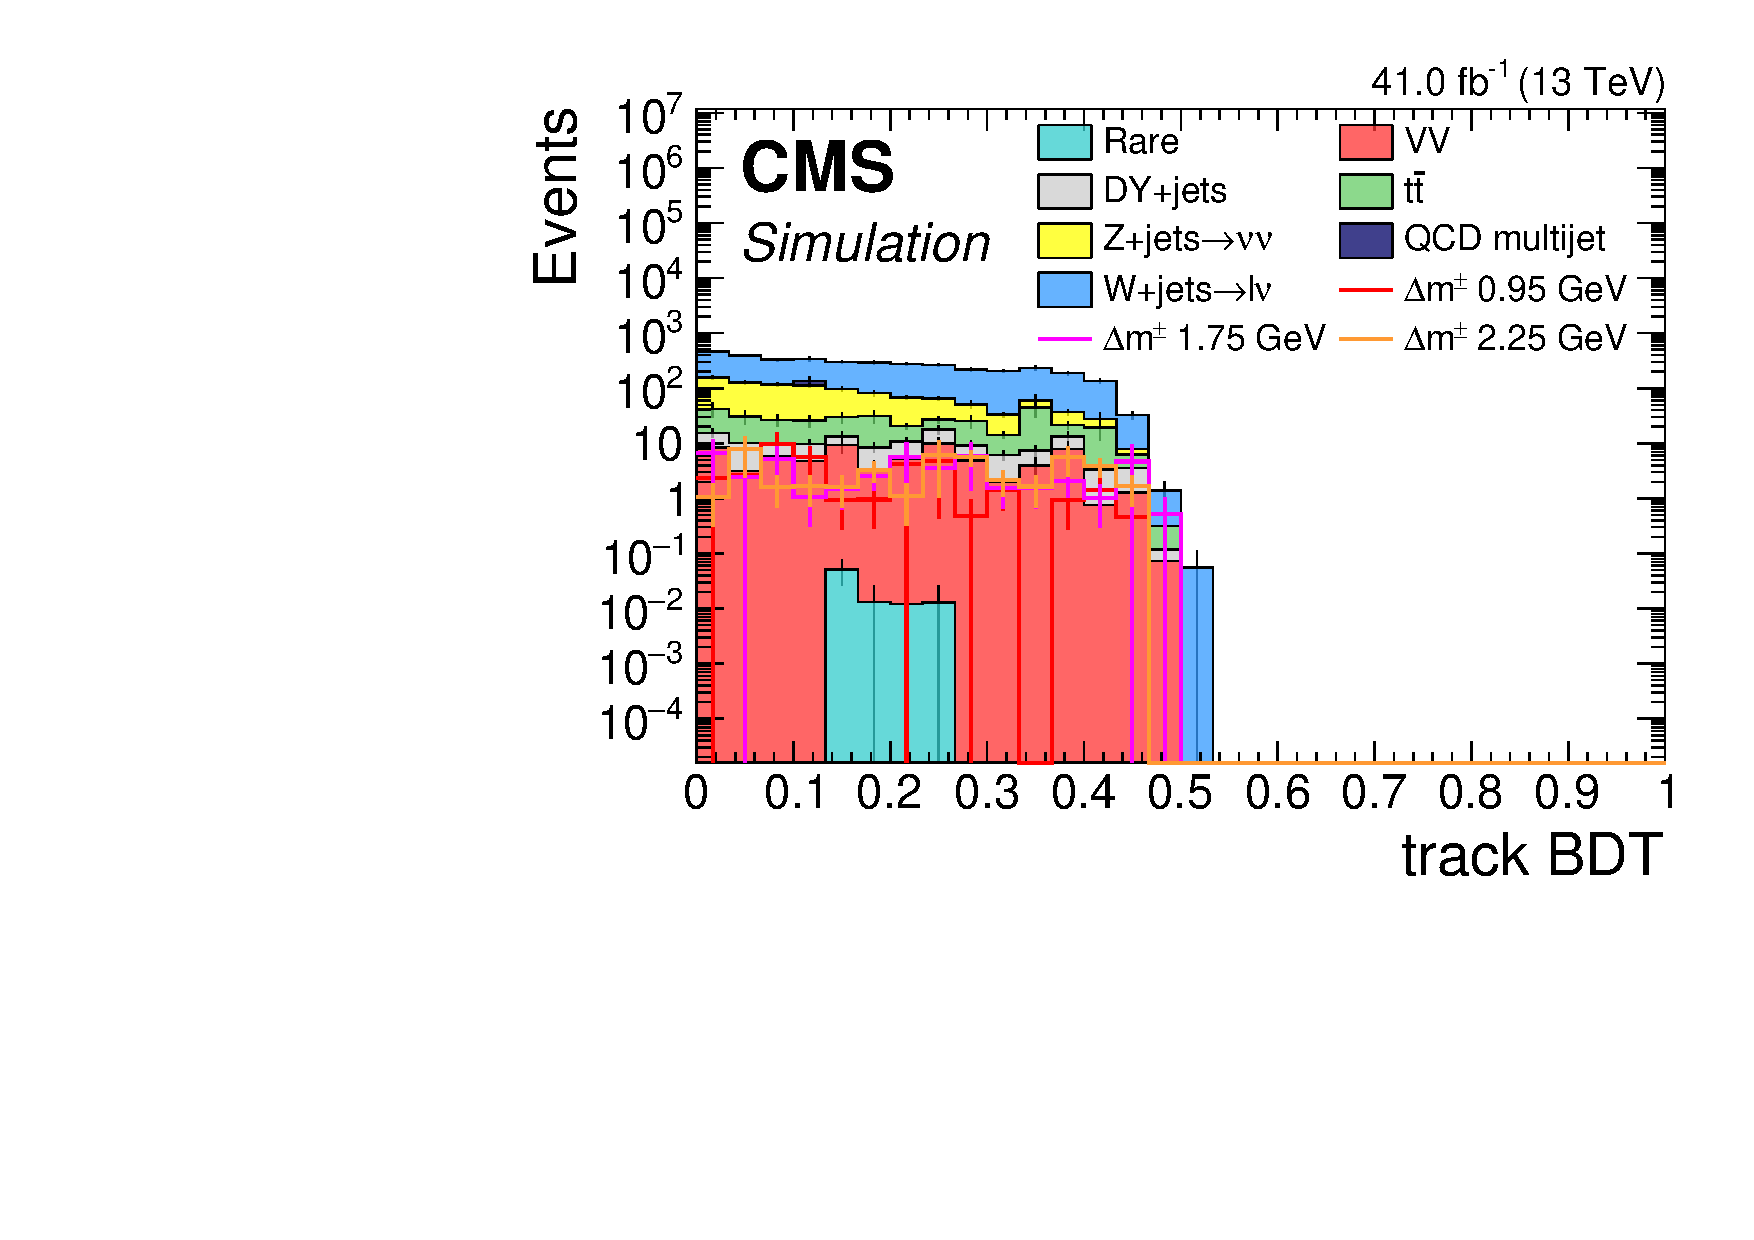
\includegraphics[width=0.48\linewidth]{plots/track_muon_bg_signal/none_trackBDTCorrJetNoMultIso10Dr0.6_log.pdf} \,
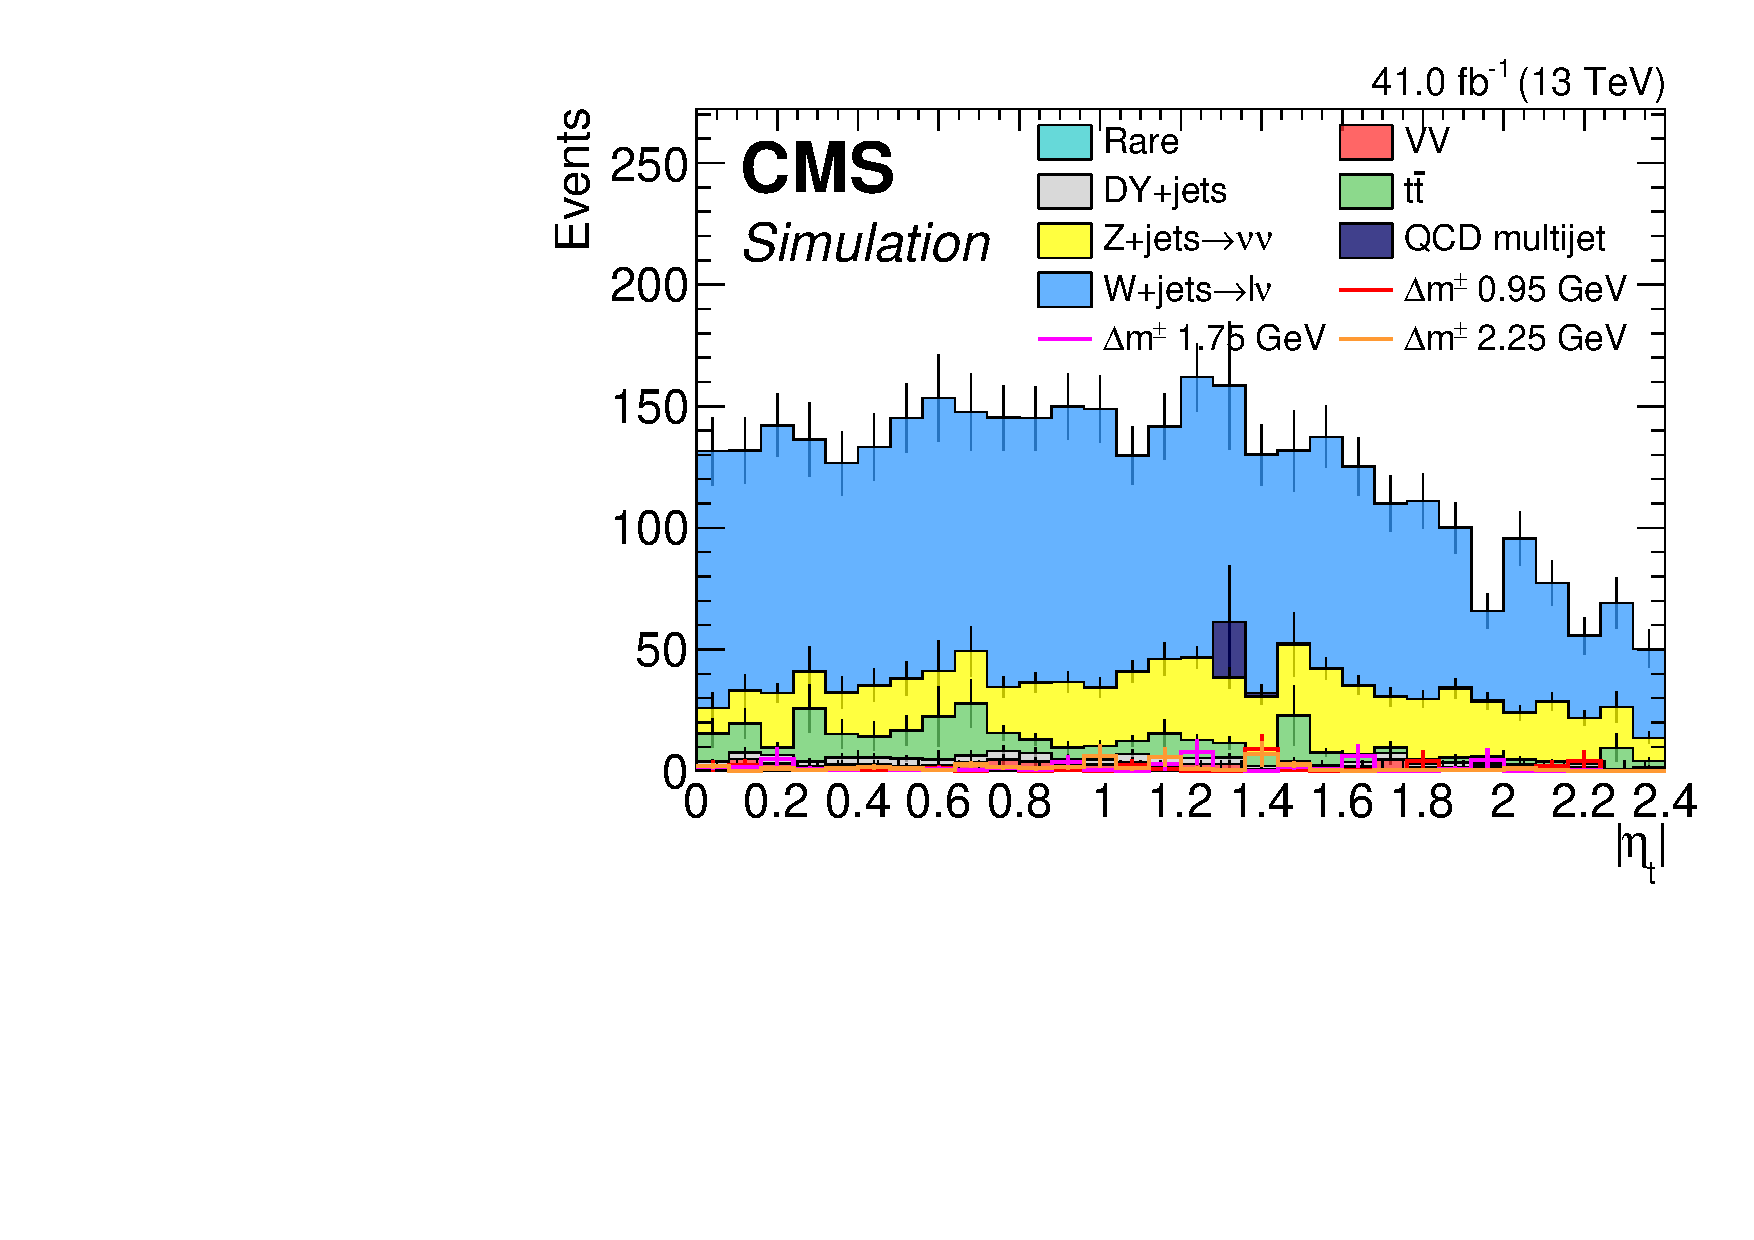
\includegraphics[width=0.48\linewidth]{plots/track_muon_bg_signal/none_abs(trackCorrJetNoMultIso10Dr0.6.Eta()).pdf} \\



\caption[Exclusive track plus muon simulation BDT inputs]{Exclusive track plus muon 2017 simulation BDT inputs for the top 8 ranked observables.}
\label{fig:exclusive-track-muon-bdt-sim-inputs}
\end{figure}


\clearpage
\subsection{Estimation of the Standard Model backgrounds}
\label{sec:background-estimation}

In analyses such as the one described in this thesis, in which new physics, or physics beyond the Standard Model is searched for, one needs to predict event counts for the signal and for the Standard Model background. These counts are denoted $s$ for the signal events count and $b$ for the background events count. From these counts and their uncertainties, a \emph{significance} is computed. The question that arises is how to predict such counts. A widely used method is \glsreset{mc}\gls{mc} simulation, sometimes simply referred to as \emph{simulation}. Prediction using simulation is pretty straight forward. First, many events are simulated using the \gls{sm} technique, taking into account the detector's geometry (by such algorithms such as \FASTSIM or \FULLSIM). They are then weighted to account for production cross sections and luminosity. Further correction factors and weights can apply to account for measurements errors, discrepancies between data and simulation, non-ideal algorithms, misidentifications, normalization corrections computed from data in a dedicated \glsreset{cr}\gls{cr}, and so forth. The nominal prediction for the events count becomes then the fully-weighted simulation count in the relevant \glsreset{sr}\gls{sr} with an uncertainty that is taken by the statistical error on the simulation count in that bin, with an optional systematic uncertainty that has been determined by other means. The signal count $s$ has been determined in this way using \FASTSIM. As is described in the following, only a small fraction of the background count $b$ has been estimated using simulation. The majority of the background processes have been estimated using \emph{data-driven methods}.

Using simulation to estimate the Standard Model background has limitations and disadvantages. These are specific to each analysis, in which the background processes composition change. The main limitation of simulation is that it is imperfect. Simulation never precisely simulates real data, and that is due to several factors. Theoretical uncertainties, such as uncertainties on cross sections or branching fractions, can lead to wrong production rate or normalization. That's why simulation is often reweighted using a normalization factor derived in a dedicated \gls{cr}. Another challenging limitation of simulation is misrepresentation of the detector's delicate geometry and response, as well as real time data-taking challenges and faults which need to be taken into account in order for the simulation to accurately represent the events that would have been recorded by the detector. Some objects and phase-spaces are more prone to discrepancies than others.

In this analysis, a great deal of the challenge arises from the very \emph{soft} nature of the leptons, \ie, their low transverse momentum \pt, as well as their low invariant mass of the order of a few\GeV. Sources of backgrounds of such events in the standard model include low-\pt resonances that are produced in hadronization processes, and events where one of the leptons (or exclusive track) is misidentified as one of the signal leptons. These leptons or tracks are often in some vicinity of jets in the event. In this analysis, there are two strategies to estimating this sort of background depending on the whether we have two identified leptons, such as in the dimuon category, or one, such as in the exclusive track category. The dimuon \emph{jetty background} estimation is described in Section~\ref{sec:jetty-background-estimation}, while the exclusive track background estimation is described in~\ref{sec:ex-track-background-estimation}. Lastly, as described earlier, small part of the background is not produced nearby jets at all, namely \ztautau. That background estimation method is described in Section~\ref{sec:mtautau-background-estimation}.

\clearpage
\subsubsection{Non-isolated jetty background estimation}
\label{sec:jetty-background-estimation}

In the description of the object selection in Section~\ref{sec:object-selection}, it has bene demonstrated that the leptons in the signal are isolated. The isolation criterion that is used in this analysis has been described in~\ref{sec:isolation}, and is referred to as \emph{jet-isolation}. It has been mentioned there that the customized isolation is also key part in the background estimation, and that is now described in this section. This background estimation method is relevant to the dimuon category. It is a \emph{data-driven} background estimation method, meaning that we use data, rather than simulation, to estimate this background. The name \emph{non-isolated jetty background} refer to background in which one or both of the leptons generally are produced in association with jets, and typically are close to one. Most of such leptons are rejected by the jet-isolation criteria, but some do manage to pass the isolation if they happen to have been produced far enough from a jet. 

Our signal regions are defined in detail in Section~\ref{sec:signal-regions}, but here it is enough to note they are bins in the \gls{bdt} output with a score greater than zero. The strategy of this method is to find a \glsreset{cr}\gls{cr} that produces a BDT output distribution that is shape-consistent with the original BDT distribution. That is achievable when a \gls{cr} can be identified such that it has almost the same features as the main region, ideally only with rate difference. Then, to get normalization correctly, one would define a normalization control region to correct for the different production rate.

Interim note on terminology should be made for clarity. The \glspl{sr} are defined by taking BDT output greater than zero, and therefore, by definition, the region with less than zero becomes a \gls{cr}. Furthermore, a new region using isolation is being introduced in this section. Since the orthogonal region only varies from the main region by isolation, it is referred to as the \emph{isolation sideband}. The main region that was used to define the \glspl{sr} using the BDT output is referred to as the \emph{main band}. The \glspl{sr} are then regions in the \emph{main band} with BDT output greater than zero. The events in the \emph{isolation sideband} are used to predict the jetty-background in the \emph{main band}. The \emph{normalization region} is taken to be in the \gls{cr} with $\mathrm{BDT}<0$, and can also be referred to as \emph{BDT sideband} or more elaborately as \emph{BDT normalization sideband}. Of course though, a \emph{sideband} is still a kind of a \gls{cr}.

Since the goal of this estimation method is to estimate the jetty-background, an isolation sideband is defined by requiring either one or two of the leptons to fail the jet-isolation criterion. That has also been defined in step 5 in Section~\ref{sec:isolation}. That means, that the lepton is distanced less than 0.6 in $\DR$ from a lepton-corrected jet. The jet that caused the lepton to fail the jet-isolation is required to have an original transverse momentum, \ie, transverse momentum before the subtractions, satisfying $15<\pt<30\GeV$. The reason why the \pt is limited to this region is because $15\GeV$ is the upper bound on the leptons, and $30\GeV$ is the lower bound on the objects being summed in the calculation of \mht and the number of jets in the event. If the upper bound of $30\GeV$ had not have been set, a bias in the isolation sideband would have been introduced, because requiring a lepton to fail jet-isolation, would also potentially mean requiring an extra jet with $\pt>30\GeV$, a requirement that didn't exist in the main band. The distributions of number of jets, as well as of \mht, are blind to jet with $15<\pt<30\GeV$, which makes it safe to potentially have extra jets in that region. The BDT training will be blind to those jets, and the BDT shape in the sideband should not be affected by those, thus achieving the goal of having consistent shapes between the main band and the sideband.

The main assumption that goes into using the isolation sideband is that in the background, the leptons are not isolated, but created in association with jets. Most will be produced inside jets, with a smoothly falling distribution outwards from a jet. By setting a cone of size 0.6 around jets and picking leptons inside those cones, events are picked up which have similar behavior to events where the leptons are outside of those cones. The rate of production of leptons inside jets will be much higher than those outside of the jets, but since their behavior is similar kinematically, by fixing the normalization, their distributions will agree with the ones in the main band. The normalization factor is calculated by taking the ratio between the main band and the isolation sideband in the \gls{cr} of $\mathrm{BDT}<0$. The event count in the sideband is multiplied by the normalization factor to comprise the prediction. The prediction in the \gls{sr} then becomes:

\begin{equation}
\mathrm{N}^{\mathrm{SR}}_{\text{predicted}} = \frac{\mathrm{N}^{\mathrm{CR}}_{\text{main band}}}{\mathrm{N}^{\mathrm{CR}}_{\text{sideband}}} \cdot\mathrm{N}^{\mathrm{SR}}_{\text{sideband}}.
\end{equation}

The assumption that the isolation sideband, \ie, events with at least one of the leptons failing the jet isolation criterion, correctly predicts the shape of the main band in the signal region, is tested by perfoming a shape comparison in simulation. Such shape comparison, or \emph{closure test}, is performed by plotting the main band and the jet isolation sideband simultaneously, and checking that they statistically agree in terms of shape. A normalization factor is computed in order to correctly normalize the isolation sideband. In the current section, treatment of phase 1 (2017-2018), which in simulation is represented by 2017 \gls{mc} is presented. Special care has been taken in the case of phase 0 (2016 data taking year) in Section~\ref{sec:systematic-uncertainties}.

\begin{figure}[!htb]
\centering
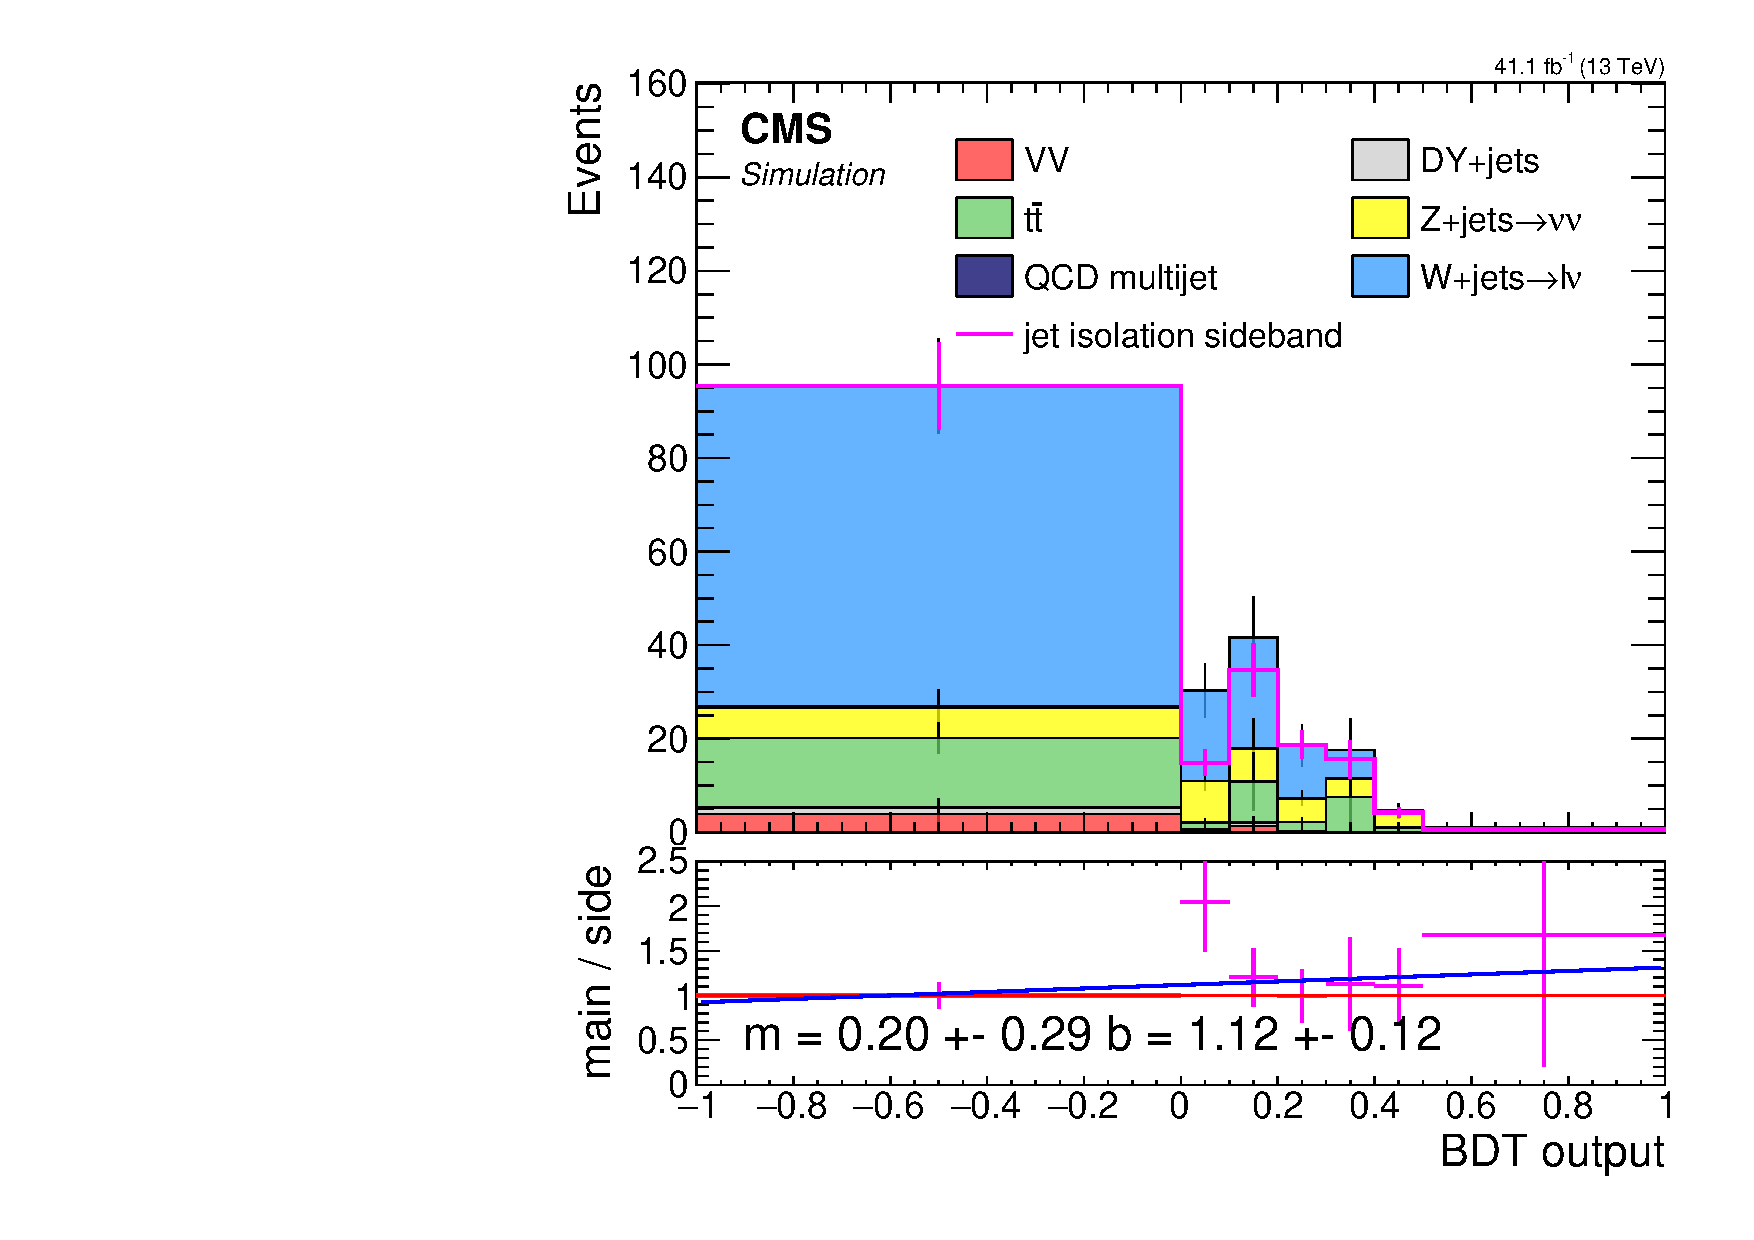
\includegraphics[width=0.60\linewidth]{plots/dilepton_muons_2017_closure/none_closure_dilepBDTphase1CorrJetNoMultIso10Dr0.6.pdf}  \\


\caption[Dimuon 2017 jetty background closure plot]{Dimuon 2017 jetty background closure plot. The stack represents simulation in the main isolation band after \ztautau has been removed, while the pink line represents simulation in the isolation sideband. The isolation sideband is normalized to match the isolation in the CR of $\mathrm{BDT} < 0$. The ratio panel shows the ratio between the isolatoin main band and sideband. A line fit of the ratio is performed and the parameters of the slope $m$ and interception point $b$ with their respective errors are stamped.}
\label{fig:dimuon-bdt-jetty-2017-closure}
\end{figure}

The jetty background closure plot is shown in Figure~\ref{fig:dimuon-bdt-jetty-2017-closure}. The closure plot tests the assumption that the background in the isolation main band can be predicted by the isolation sideband. Therefore, after proper normalization that is achieved by dividing the event count in the the main band with the event count in the sideband, which in this case is 0.59, a flat ratio distribution is to be expected in the \glspl{sr}. One can observe that indeed such a flat ratio distribution has been achieved by noting that most bins are statistically consistent with unity. To check for any trend, a line fit has been performed for the ratio panel. Taking into account the errors, up to $1\sigma$, the slope $m$ is consistent with 0 and the interception $b$ is consistent with 1, making the line consistent with a flat line intercepting 1. It is to be concluded therefore, that the closure plot confirms the shape assumption, and no trend that needs to be taken into account is to be seen. Full list of transfer factors with the associated uncertainties are found in Section~\ref{sec:data-driven-tranfer-factors}, while special treatment of the 2016 case can be seen in Section~\ref{sec:data-driven-shape}.

\subsubsection{Ditau Drell-Yann background estimation}
\label{sec:mtautau-background-estimation}

It has been seen in Section~\ref{sec:dimuon-category-background-char} that the majority of the standard model background is composed of processes that produce leptons in association with jets, and therefore can be estimated with the jetty-background data-driven estimation method described in Section~\ref{sec:jetty-background-estimation}. However, as can be seem in Figure~\ref{fig:dimuon-bdt-sim-output-jetty-tautau}, a small amount of background arising from \ztautau is also present, and since the leptons due to the leptonic decay \tautomu are isolated, it requires an alternative background estimation method.

The \ztautau background in this category is estimated using \gls{mc} simulation. The event counts is being weighted according to a data correction normalization factor calculated in a dedicated \gls{cr}. In order to do so, a \gls{cr} rich and relatively pure in \ztautau background must be found. In order to achieve this task, the observable \mtautau must be introduced. The background in question is due to a Drell-Yann process where a \PZ is decaying into two tau leptons, which in turn decay into muons via \tautomu. If the taus could be reconstructed, they could be used to calculate the invariant mass of the ditau event, \mtautau, which is expected to peak at around the \PZ mass. The \PZ resonance could then be used as the desired \gls{cr} rich in ditau background. However, leptonic taus are not directly reconstructed at \gls{cms}, which makes it necessary to find an alternative approach for calculating said invariant mass.

A widely used method for the reconstruction of the invariant mass \mtautau is the so-called \emph{collinear approximation}. First described in~\cite{ELLIS1988221_first_mtautau}, it has been used widely in \acrshort{atlas}~\cite{ATLAS:2009zsq} and \acrshort{cms}~\cite{CMS:2007sch}. In the collinear approximation, one assumes that the tau pair produced from \PZGammaStar are highly energetic, so that their leptonic decays are collinear and the source of missing transverse momentum is due to the neutrinos only. If both the $\PGt$-letpons are sufficiently boosted, the neutrinos from each \PGt decay are collinear with the
visible lepton momentum. One can then use the visible daughter-lepton momentum together with \ptvecmiss to reconstruct the $\PGt$-lepton pair and calculate the would-be \mtautau invariant mass. Depending slightly on the mathematical details of the approximation, one can arrive at a strictly positive distribution for \mtautau, as was done for example in~\cite{Han_2014_positive}, or one that also has negative values, as was done in~\cite{Baer_2014_negative,Barr_2015_diff}. Since the negative values arising from the second variation of the approximation are due to events where \ptvecmiss points away from one of the leptons, and therefore not arising from underlying boosted ditau events, it is useful to reject negative values in order to purify the \gls{cr} by rejecting those events. The collinear approximation does not work when the taus are back-to-back. However, since in this analysis an \gls{isr} jet is required together with a high threshold of missing transverse momentum, it is expected to work well on the remaining boosted events. The signal, as well as other standard model processes are expected to have a flat distribution in \mtautau, while events arising due to \ztautau are expected to peak around the \PZ boson mass.

To put the assumptions into practice, an explicit definition of \mtautau is now laid out. The definition of the invariant mass is:

\begin{equation}
\label{eq:mtautau}
\mtautau^2 = (p_{\PGt_1} + p_{\PGt_2})^2
\end{equation}

Assuming that the $\PGt$-pair is boosted, and the fully-lepotonic decaying products is fully collinear to the $\PGt$-leptons, it follows that the transverse momentum of each neutrinos-pair is proportional to the corresponding $i$ $\PGt_i$'s transverse momentum by a scale-factor $\xi_i$ by 
\begin{equation}
\vec{\pt}^{\PGn_i}=\xi_i \vec{\pt}^{\PGt_i}
\end{equation}

Since by assumption, all of the missing transverse momentum is due to the neutrinos, it follows that:

\begin{equation}
\label{eq:two-mtautau}
\ptvecmiss =\xi_1 \vec{\pt}^{\PGt_1}+\xi_1 \vec{\pt}^{\PGt_2}
\end{equation}

One solves the above two equations~\ref{eq:two-mtautau} for the two parameters $\xi_1$ and $\xi_2$ for each event. The solution becomes:

\begin{equation}
\begin{split}
\xi_1 = \frac{{{\vec p}_{\mathrm{T}_x}^{\kern1pt\text{miss}}} \cdot {\vec p}_y^{\ell_2}  - {{\vec p}_{\mathrm{T}_y}^{\kern1pt\text{miss}}} \cdot {\vec p}_x^{\ell_2}  }{ {\vec p}_{x}^{\ell_1} \cdot {\vec p}_{y}^{\ell_2} -  {\vec p}_{x}^{\ell_2} \cdot {\vec p}_{y}^{\ell_1} },\\
\xi_2 = \frac{{{\vec p}_{\mathrm{T}_y}^{\kern1pt\text{miss}}} \cdot {\vec p}_x^{\ell_1}  - {{\vec p}_{\mathrm{T}_x}^{\kern1pt\text{miss}}} \cdot {\vec p}_y^{\ell_1}  }{ {\vec p}_{x}^{\ell_1} \cdot {\vec p}_{y}^{\ell_2} -  {\vec p}_{x}^{\ell_2} \cdot {\vec p}_{y}^{\ell_1} }.
\end{split}
\end{equation}

Equation~\ref{eq:mtautau} is expended with the assumption that the $\PGt$'s are boosted and that the four-momenta of the taus is $p_{\PGt_i} = (1+\xi_i)p_{\ell_i}$:

\begin{equation}
\label{eq:mtautau-approx}
\begin{split}
\mtautau^2 &= ({p_\PGt}_1 + {p_\PGt}_2)^2 \\
&=\left((1+\xi_1){p_\ell}_1+(1+\xi_2){p_\ell}_2\right)^2\\
&=2m_\PGt^2+2(1+\xi_1)(1+\xi_2){p_\ell}_1\cdot {p_\ell}_2\\
&\approx 2(1+\xi_1)(1+\xi_2){p_\ell}_1\cdot {p_\ell}_2.
\end{split}
\end{equation}

This can be negative is $\xi_i < -1$. This can happen if the missing transverse momentum vector nearly opposite to a lepton's \ptvec and also $\ptmiss > \pt^\ell$. This can easily happen in other background processes, such as $\mathrm{WW}$+jets , when a neutrino and a lepton (possibly coming
from different decay legs) are nearly back-to-back. Therefore, the final definition of \mtautau is

\begin{equation}
\mtautau = \mathrm{sign}(\mtautau^2)\sqrt{\abs{\mtautau^2}}.
\end{equation}

The \gls{cr} to be used for the normalization should potentially have low signal contamination. It can be seen in Figure~\ref{fig:dimuon-bdt-sim-output} that the region of $\text{BDT} < 0$ has hardly any signal contamination, and therefore is used for building the \tautau \gls{cr}. Figure~\ref{fig:mtautau-distributions} shows distributions of the \mtautau for the \tautau simulation in red, and the rest of the standard model backgrounds in the stack. The two tracker phases are seen side by side. There is a clear peak in the \tautau background at around the \PZ boson's mass. A window around the \PZ boson's mass is chosen of $[40,130]\GeV$ in order to achieve high purity of 73\% in both phases. The contamination in data is removed by first predicting the jetty background count using the data-driven method described in Section~\ref{sec:jetty-background-estimation}, and subtracting those counts from the data counts in the \tautau dedicated \gls{cr}. Then, a data divided by simulation normalization factor is computed in said \mtautau window to get $1.2\pm 0.46$ ($0.29\pm 0.26$) which has relative error of 38\% (90\%) for phase 0 (phase 1).

\begin{figure}[!htb]
\centering
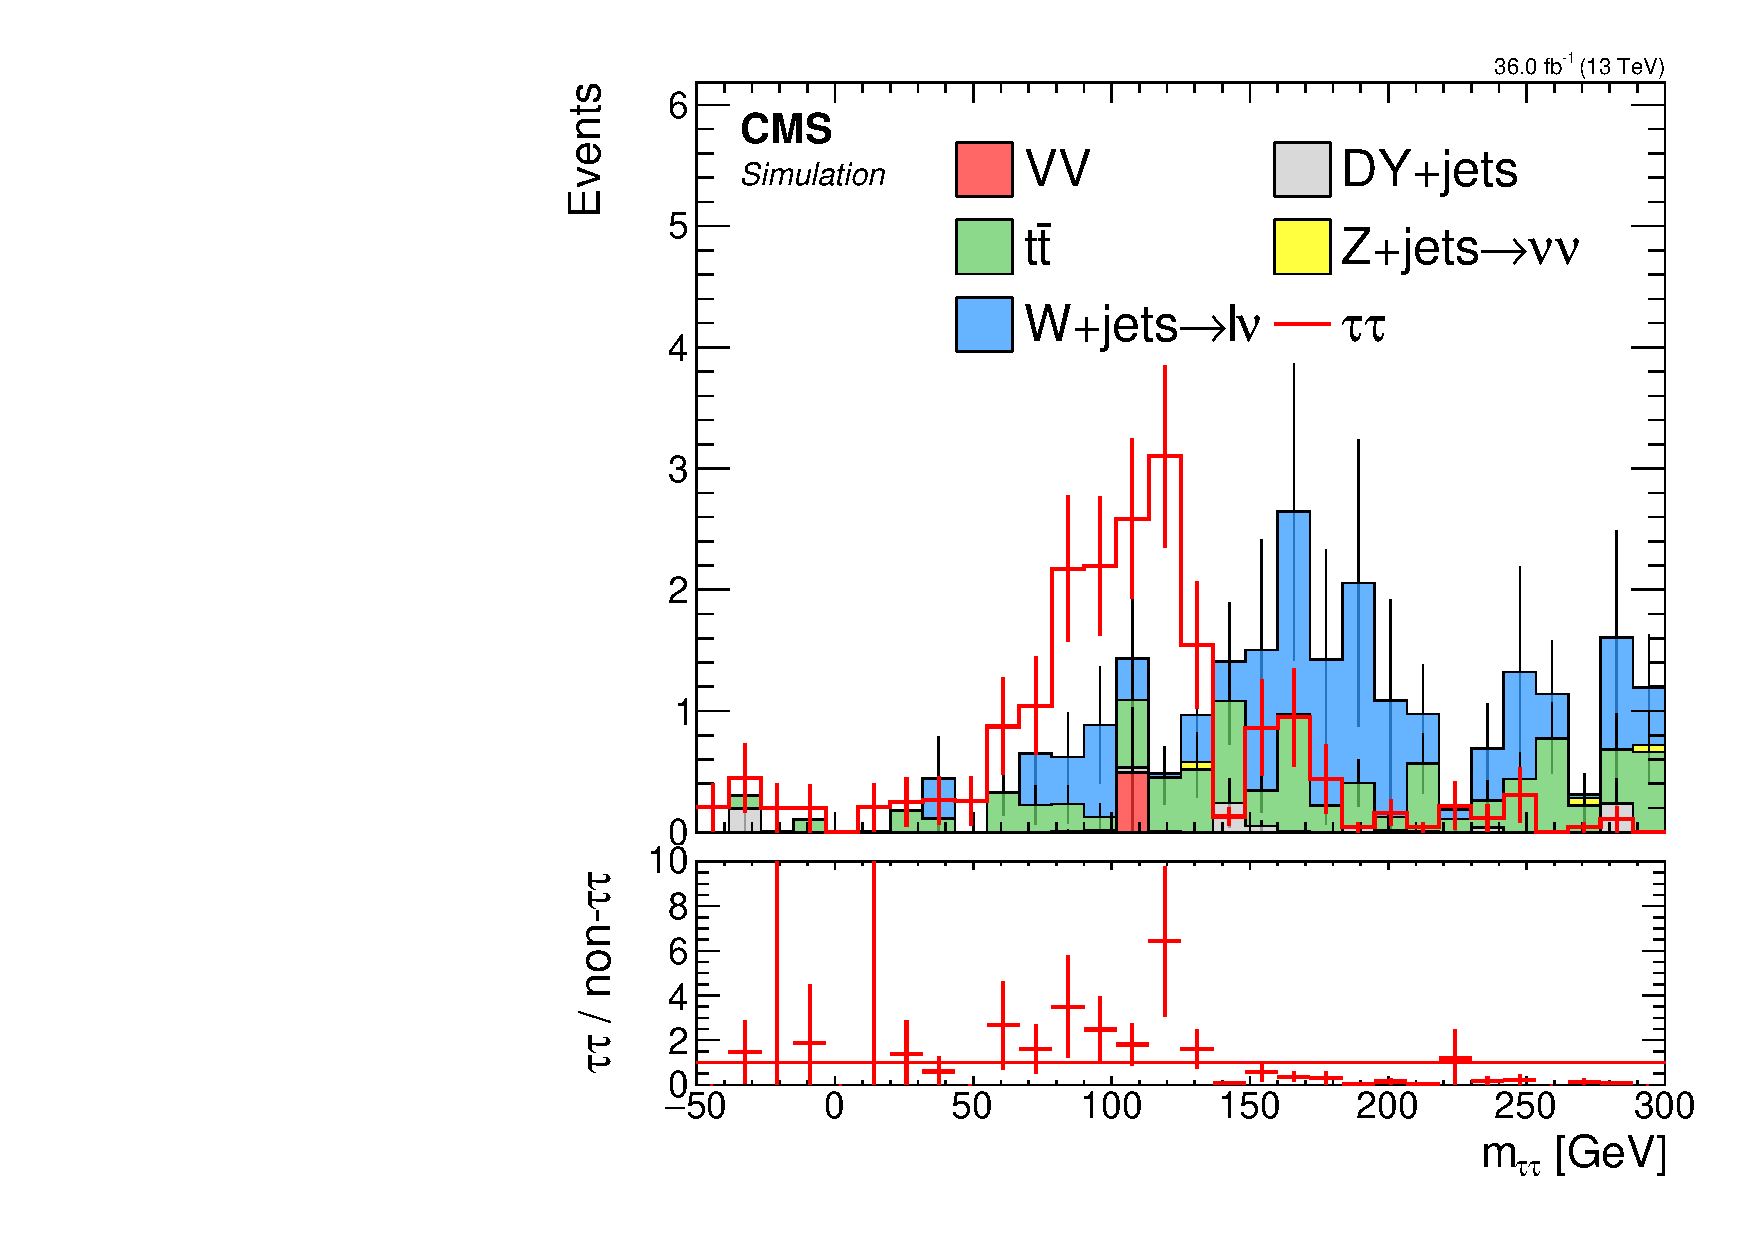
\includegraphics[width=0.48\linewidth]{plots/dilepton_muons_bg_isocr_scan_tautau_vs_no_tautau/bdt2_nmtautauCorrJetNoMultIso10Dr0.6.pdf} \,
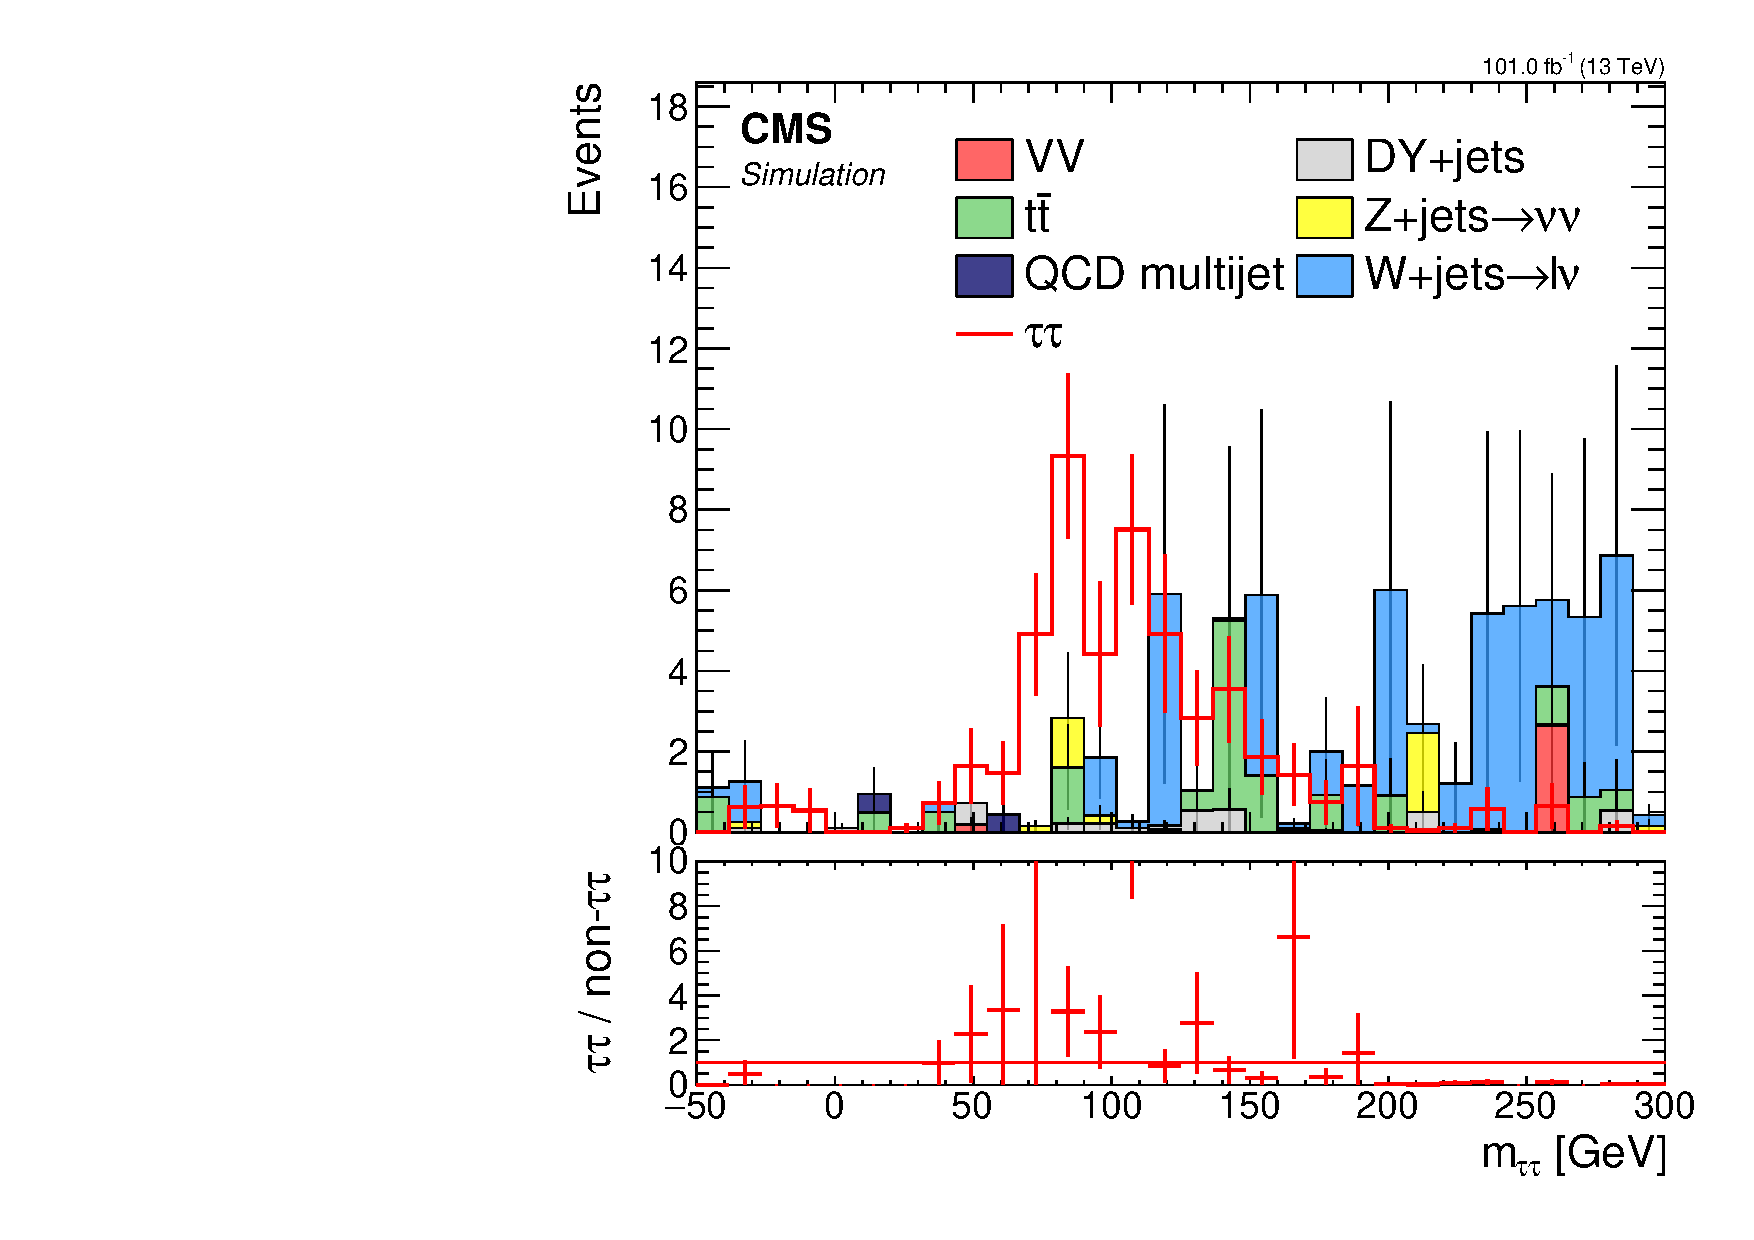
\includegraphics[width=0.48\linewidth]{plots/dilepton_muons_bg_isocr_scan_tautau_vs_no_tautau_phase1/bdt_nmtautauCorrJetNoMultIso10Dr0.6.pdf} \\


\caption[Ditau invariant mass distibutions]{Ditau invariant mass \mtautau distributions for phase 0 2016 simulation (left) and phase 1 2017 simulation weighted to luminosity of 2017-2018 data taking period (right). The red line corresponds to \tautau simulation, and the stack represents the rest of the standard model background simulation. No overflow bins are plotted in order to clearly show the resonance peak.}
\label{fig:mtautau-distributions}
\end{figure}

\clearpage
\subsubsection{Exclusive track background estimation}
\label{sec:ex-track-background-estimation}

The exclusive track category is consisted of four different \glspl{bdt}, one for each lepton flavor and for each of those one for each phase. However, the background estimation method is the same for all of them, and it is a data-driven one.

The exclusive track category required one fully identified lepton according to the selection listed in Sections~\ref{sec:object-selection-electrons} and~\ref{sec:muon-selection}, and one track by a procedure described fully in Section~\ref{sec:track-bdt}. The track that is selected to be paired with the single identified lepton is selected as the track in the event with the highest \gls{bdt} score among all tracks using a \gls{bdt} that was trained on signal events in order to reject in-signal background and potentially pick up the track that corresponds to the non-identified second lepton in the signal event. In the background, the same selection procedure applies. However, unlike in the signal, it cannot be expected that the pairing of the selected track has a special relationship to the identified lepton other than passing some selections on the phase space. The chance of selecting a track in the background, that in combination with the identified lepton  form an opposite-sign same-flavor pair that is a result of a resonance decay, is vanishingly small. It is highly likely that the track corresponds either to a lepton produced independently of the identified lepton in the event, or that it doesn't correspond to a lepton at all. Such as track is referred to as a \emph{fake} track, and almost all tracks in the event are fakes.

To devise a successful data-driven background estimation for the exclusive track category we take advantage of the fact that the tracks in the background are independent of the identified lepton in the event. The selection process considered only tracks with opposite charge to the identified lepton, but if the track is independent of the lepton, events with a track of the same charge will be picked at the same rate as opposite charge ones. Not only is it expected to be selected at the same rate, but the shape of the \gls{bdt} output will also be blind to this choice, making it an excellent proxy to the opposite charge background.

A \gls{cr} is defined by selecting same-charge lepton-track pair rather then opposite-charge as in the \gls{sr}. It is expected that the same charge \gls{cr} is consistent also by the normalization to the \gls{sr} since it is expected that these events are selected at the same rate of each other. Despite of this, the normalization is fixed by calculating a normalization factor as the ratio between the opposite-charge to same-charge event count in a dedicated normalization sideband \gls{cr} satisfying $\text{BDT} < 0$, and applying it to the same-charge event count in the \glspl{sr} satisfying $\text{BDT} > 0$. In order to test the independence assumption and to demonstrate the correct shape and normalization prediction, a closure test is performed in simulation. Figure~\ref{fig:ex-track-closure-tests} demonstrates closure tests for muons and electrons for both tracker phases. The stack represents standard model background for opposite-charge analysis selection lepton-track pair (oc), while the orange line represents same-charge lepton-track pair (sc). Both are weighted to represent each phase's luminosity. In the ratio panel, which shows the ratio between opposite-charge to same-charge backgrounds for each bin, a shape agreement is demonstrated which supports the assumptions made above.

After establishing that the method can be used to correctly predict the background, a data-driven normalization factor, which is computed as the ratio between opposite-charge to same-charge data event count in the \gls{cr} of $\text{BDT} < 0$. The final prediction in the \glspl{sr} then becomes the same-charge data event count in the \gls{sr} multiplied by the normalization factor. The computed normalization factor for phase 0 (2016) is $1.12\pm 0.044$ ($1.037\pm 0.05$) for muons (electrons), and for phase 1 (2017-2018) is $1.066\pm 0.024$ ($1.049\pm 0.03$) for muons (electrons). The relative errors on the normalization factors are between 2\% to 5\%.


\begin{figure}[!htb]
\centering
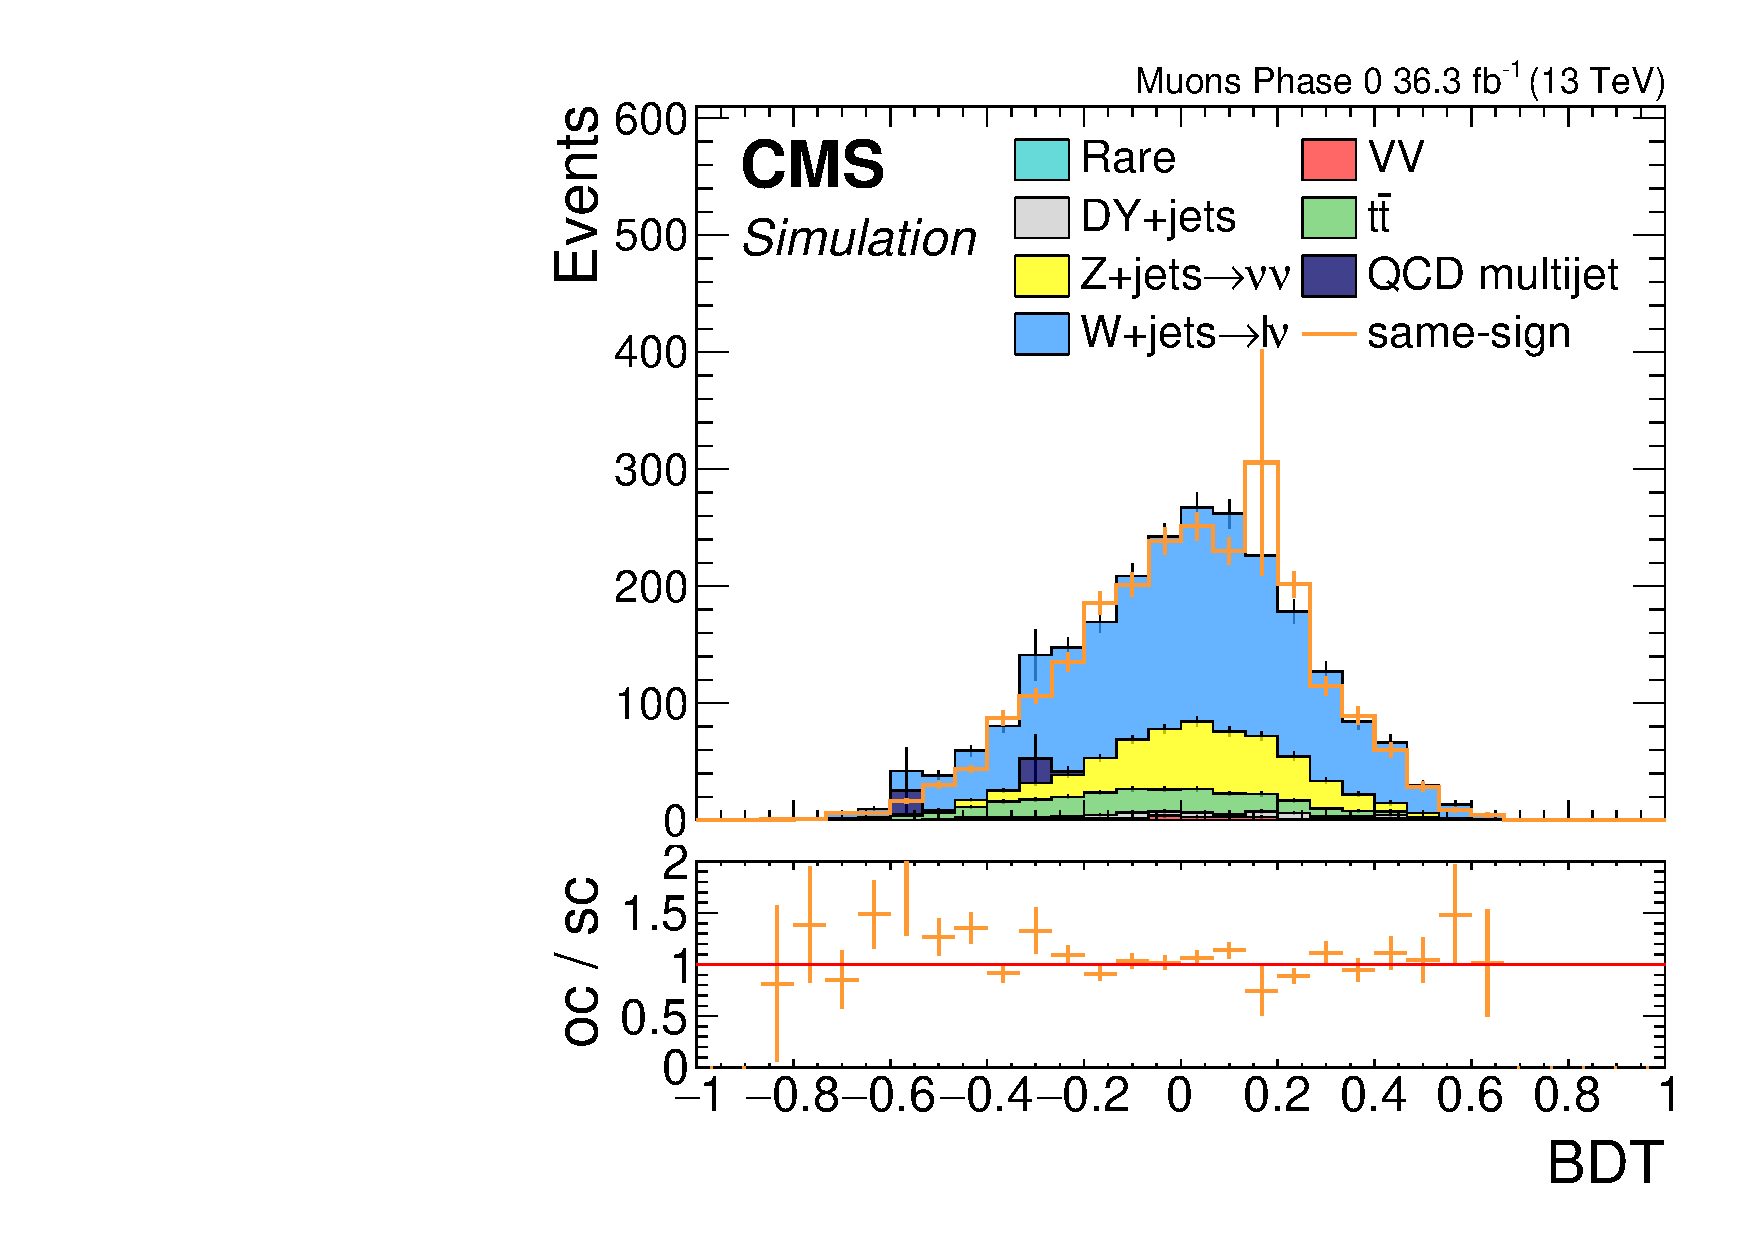
\includegraphics[width=0.48\linewidth]{plots/track_muon_sc_comparison/none_exTrack_dilepBDTCorrJetNoMultIso10Dr0.6.pdf} \,
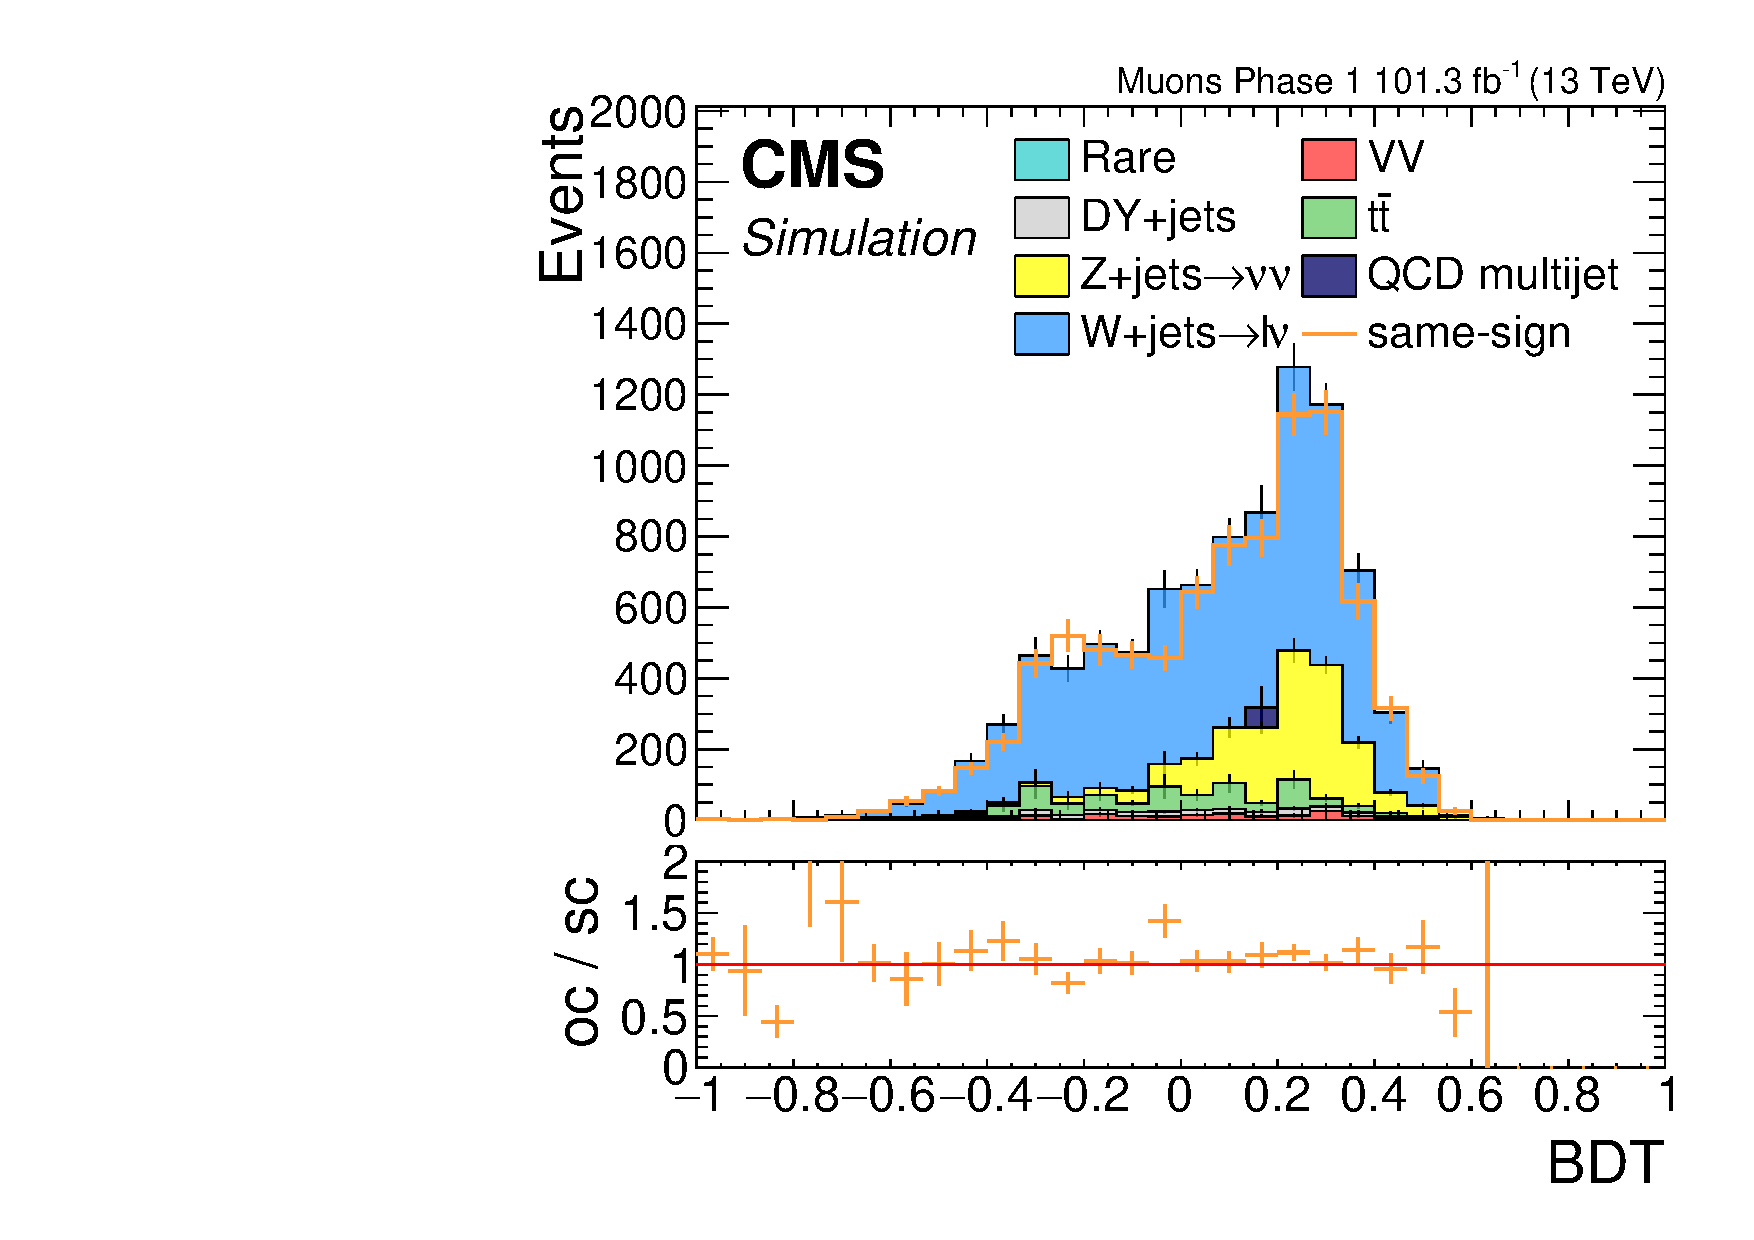
\includegraphics[width=0.48\linewidth]{plots/track_muon_sc_comparison_phase1/none_exTrack_dilepBDTCorrJetNoMultIso10Dr0.6.pdf}  \\
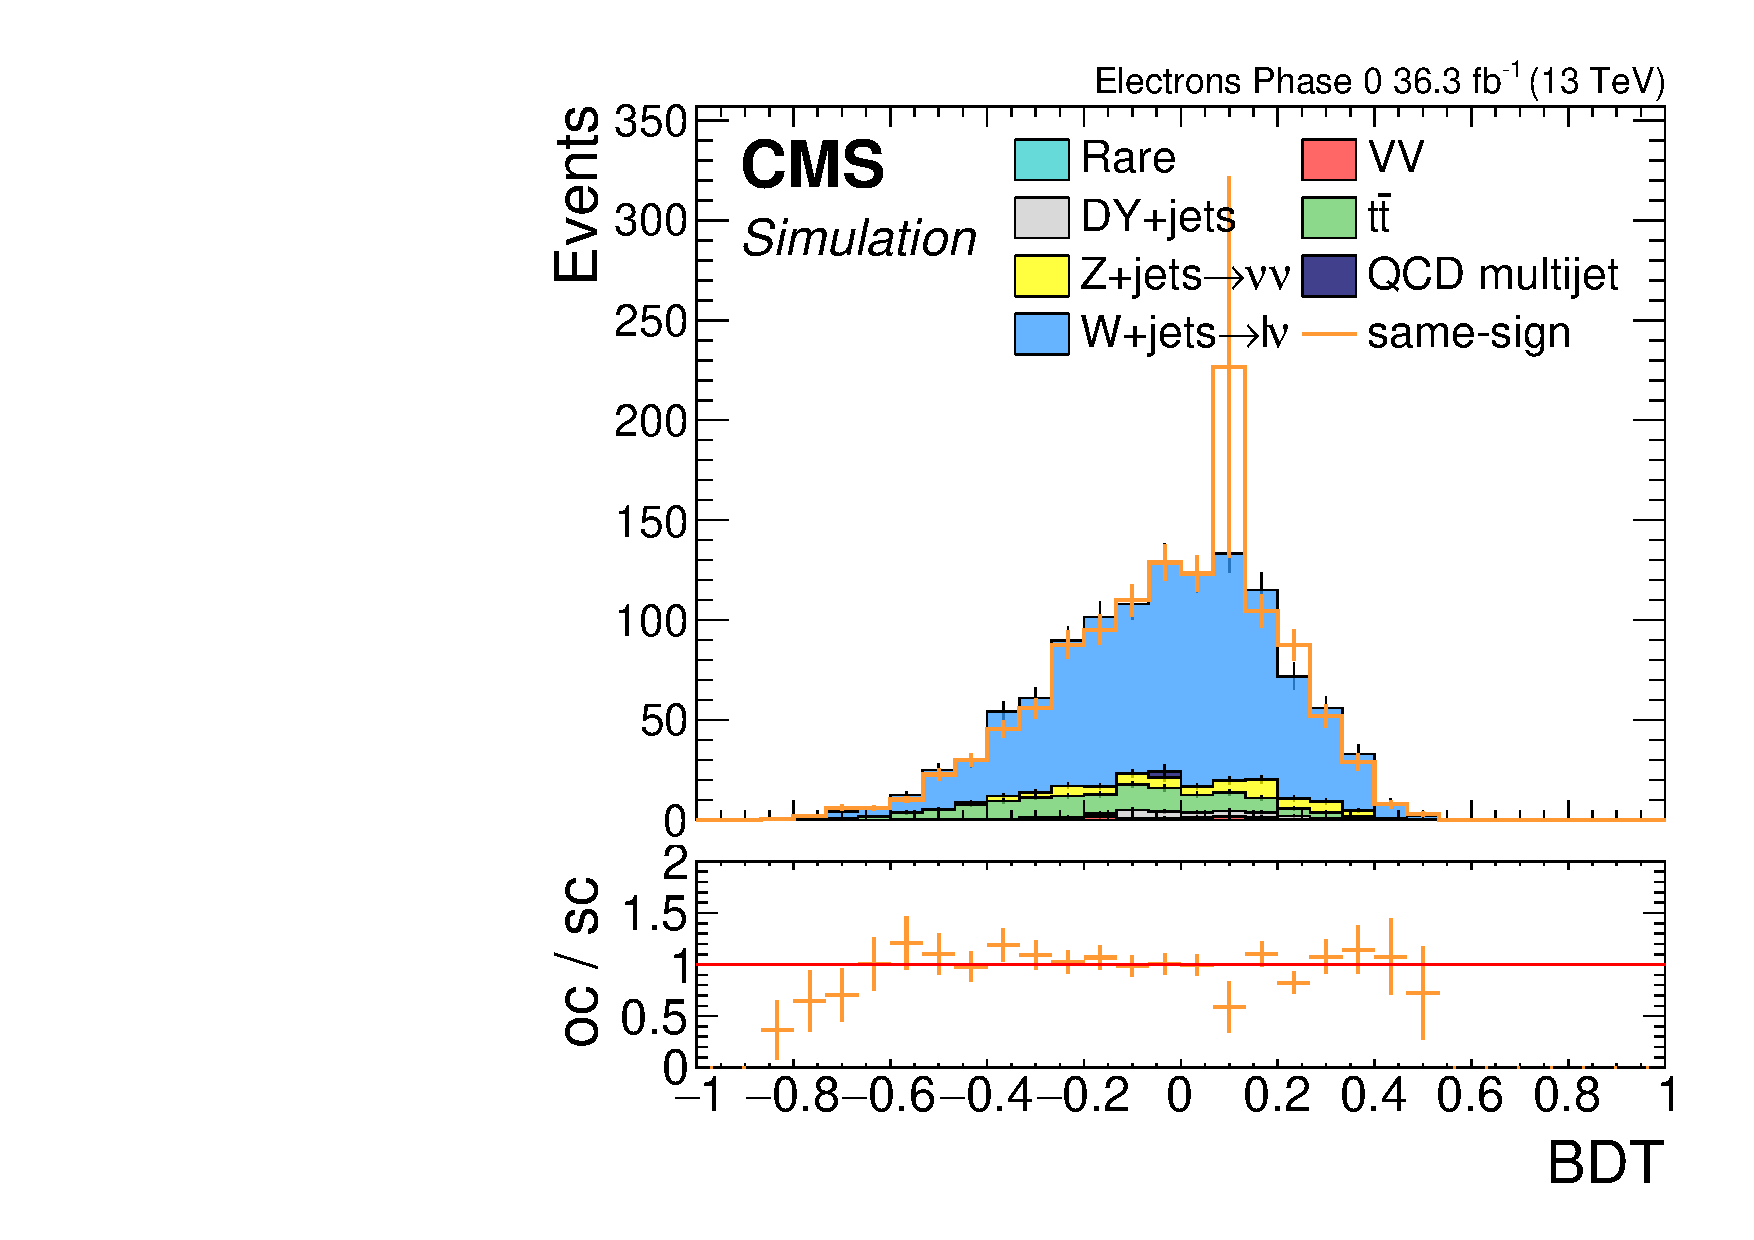
\includegraphics[width=0.48\linewidth]{plots/track_electron_sc_comparison/none_exTrack_dilepBDTCorrJetNoMultIso10Dr0.5.pdf} \,
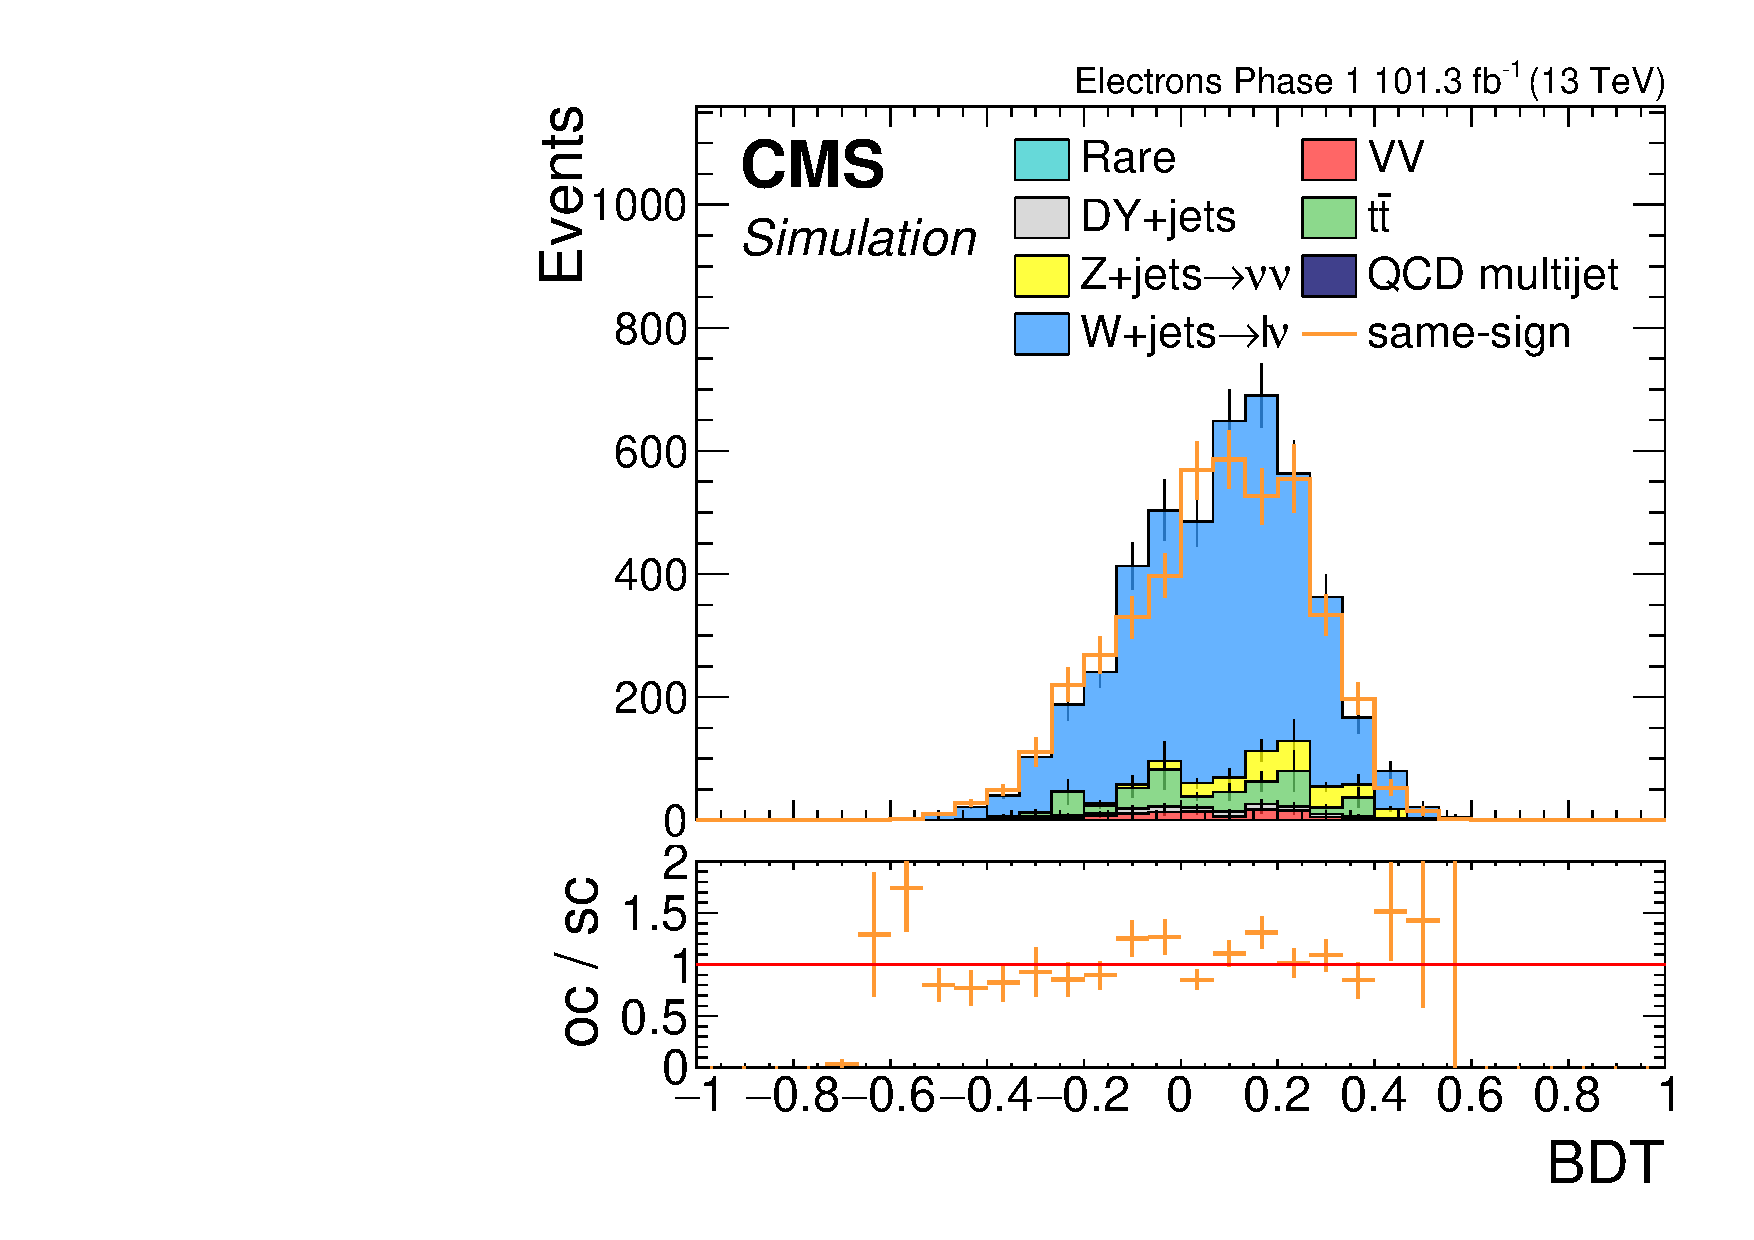
\includegraphics[width=0.48\linewidth]{plots/track_electron_sc_comparison_phase1/none_exTrack_dilepBDTCorrJetNoMultIso10Dr0.5.pdf} \\
\caption[Exclusive track category closure tests]{Exclusive track category closure tests for muons (top) and electrons (bottom) for phase 0 (left) and phase 1 (right). The stack represents standard model background for opposite-charge analysis selection lepton-track pair (oc), while the orange line represents same-charge lepton-track pair (sc). Both are weighted to represent each phase's luminosity. The ratio panel shows the ratio between opposite-charge to same-charge backgrounds for each bin.}
\label{fig:ex-track-closure-tests}
\end{figure}